\def\fileversion{v2.25a} \def\filedate{2009/10/10}
%% Package and Class "uiucthesis2009" for use with LaTeX2e.

\documentclass[edeposit,fullpage,draftthesis]{uiucthesis2009}

\usepackage[letterpaper, margin=1in]{geometry}
\usepackage{graphicx}
\usepackage{amsmath}

% for quotations
\usepackage{epigraph}

\usepackage[numbers, square, sort]{natbib}

\usepackage{hyperref}
\usepackage[toc,page]{appendix}

% so that figures are numberd per chapter.section, ie 4.1.1, 4.1.2
%\usepackage{chngcntr}
%\counterwithin{figure}{section}

% thai character stuff
\usepackage[thai,english]{babel}
\usepackage[utf8x]{inputenc}

\newcommand{\code}[1]{\texttt{#1}}

% Hack into CJKutf8 package for an option clash error
%\makeatletter
%\@namedef{opt@inputenc.sty}{utf8}
%\makeatother
%\usepackage{CJKutf8}

\begin{document}

\title{Substrate-Mediated Modulations of Graphene's Electronic Properties}
\author{John Henry Hinnefeld}
\department{Physics}
\phdthesis
\advisor{Nadya Mason}
\degreeyear{2016}
\committee{
Professor S. Lance Cooper, Chair\\
Associate Professor Nadya Mason, Director of Research\\
Assistant Professor Arend van der Zande \\
Professor Emeritus Richard Weaver}
\maketitle

\frontmatter

%% Create an abstract that can also be used for the ProQuest abstract.
%% Note that ProQuest truncates their abstracts at 350 words.
\begin{abstract}
This is a comprehensive study of caffeine consumption by graduate
students at the University of Illinois who are in the very final
stages of completing their doctoral degrees. A study group of six
hundred doctoral students\ldots.
\end{abstract}

%% Create a dedication in italics with no heading, centered vertically
%% on the page.
\begin{dedication}
To my family.

\foreignlanguage{thai}{\textthai{หนังสน้อยือี}}

\end{dedication}

%% Create an Acknowledgements page, many departments require you to
%% include funding support in this.
\chapter*{Acknowledgments}

Whenever anyone asks me for advice about graduate school the first thing
I say is ``Find a good advisor.'' Nothing has a larger impact on your quality
of life as a graduate student than your advisor, and I have been incredibly fortunate
to have Nadya as mine. Grad school is a time to learn and 
grow as a scientist and researcher, and I certainly have, but I've also grown as a person
during this time by having a broad and meaningful life outside of lab.
Many, many thanks to Nadya for creating an environment and fostering relationships with all
of us in the group that made this possible.

Thanks to everyone in the group too -- Nick who convinced me to come to UIUC and join
the lab in the first place, Scott for showing me the ropes in the beginning, Serena and Clare 
for modeling the persistence it takes to graduate, Malcolm for always knowing how
everything in the lab works, Jeff and Stephen for their Statler-and-Waldorf style take
on lab stuff, Angela and Rita for commiserating about failed experiments, Sungjae, Joe, Yingjie,
and Vincent for their advice from the other side, and Greg and Junseok for keeping things going.

Thanks to everyone in both of the bands -- Adrian, Jackson, Matt, Alex, and Apoorv,
Venanzio, Nate, Ariel, Sergio, and Carlos. First, for putting up with me as I
was learning the fiddle, and then for being so much fun to make music with.
Of all the things (bar one) that I did in graduate school, making music
with all of you was far and away my favorite.

Mondays at the Hootenanny, \textit{mulats\'{a}gs} at Apoorv's place till the wee hours of the morning,
cookouts in the summer and hot-pots in the winter,

My wife (!) Nadha

%% The thesis format requires the Table of Contents to come
%% before any other major sections, all of these sections after
%% the Table of Contents must be listed therein (i.e., use \chapter,
%% not \chapter*).  Common sections to have between the Table of
%% Contents and the main text are:
%%
%% List of Tables
%% List of Figures
%% List Symbols and/or Abbreviations
%% etc.

\setcounter{tocdepth}{2}

\tableofcontents
\listoftables
\listoffigures

%% Create a List of Abbreviations. The left column
%% is 1 inch wide and left-justified
\chapter{List of Abbreviations}

\begin{symbollist*}
\item[CA] Caffeine Addict.
\item[CD] Coffee Drinker.
\end{symbollist*}

%% Create a List of Symbols. The left column
%% is 0.7 inch wide and centered
\chapter{List of Symbols}

\begin{symbollist}[0.7in]
\item[$\tau$] Time taken to drink one cup of coffee.
\item[$\mu$g] Micrograms (of caffeine, generally).
\end{symbollist}

\mainmatter
\chapter{Introduction}

   \epigraph{God created the bulk; surfaces were invented by the devil.}{Wolfgang Pauli}
    

    \section{Motivation}
    \section{Statement of thesis problem}


\chapter{Background}

    Since its initial isolation in 2004 graphene has been the subject of intense research interest. 
    The following chapter presents a summary of the relevant properties and research results 

    \section{Introduction to graphene}

    Much of graphene's interesting behavior comes from its unique, two-dimensional structure. 
    This unique structure gives graphene a variety of interesting characteristics, however a complete 
    description of its attributes is beyond the scope of this report. Those properties of graphene 
    which are relevant to the research comprising this thesis are summarized below; for a more complete description 
    of graphene see one of the existing review articles \cite{Geim2007}, \cite{CastroNeto2009}. 
    Here I discuss graphene's band structure and several relevant consequences, namely 
    the massless Dirac fermion character of charge carriers in graphene, 
    the unique variant of the quantum Hall effect these carriers give rise to, 
    and the presence of Klein tunnelling.
    I also discuss the means and effects of doping and straining graphene. The latter discussion (of strain)
    includes a description of graphene's mechanical properties as well as the optical signatures of 
    lattice vibrations in graphene.
    
    \begin{figure}
    \centering
    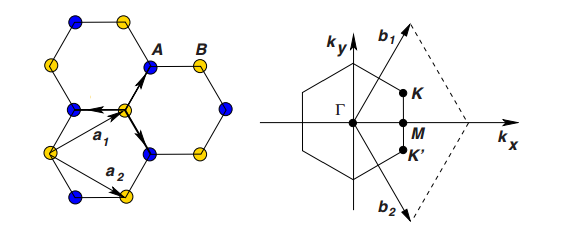
\includegraphics{images/background/ElecPropertiesFig2.png}
    \caption[The lattice structure of graphene and its Brillouin zone]{The lattice structure of graphene and its Brillouin zone. Left: Graphene is composed of two interlaced triangular sublattices, labelled \textbf{A} and \textbf{B}. Each sublattice has unit vectors $a_1$ and $a_2$. Right: The Brillouin zone of graphene has several high symmetry points. In particular, the points \textbf{K} and \textbf{K'} are referred to as Dirac points. Adapted from \cite{CastroNeto2009}.}
    \label{fig:lattice}
    \end{figure}
		
	\subsection{Band structure}
    As illustrated in Figure \ref{fig:lattice}, graphene is composed of carbon atoms in a hexagonal lattice. The hexagonal lattice contains two interlaced triangular lattices, labelled \textbf{A} and \textbf{B}. Each individual sublattice has unit vectors $a_1$ and $a_2$. The Brillouin zone of graphene's lattice is also illustrated in Figure \ref{fig:lattice}; the corners, indicated by the labels \textbf{K} and \textbf{K'} are referred to as Dirac points for reasons described below. 
    The band structure of graphene is shown in Figure \ref{fig:bandstructure}; undoped graphene is a zero-gap semiconductor. This band structure is calculated using a simple tight-binding model, with a Hamiltonian (using units where $\hbar=1$) \cite{CastroNeto2009}:
    \begin{equation}
    H = - t \sum\limits_{\langle i,j\rangle,\sigma} (a_{\sigma,i}^\dagger b_{\sigma,j} + \text{H.c.})
    - t' \sum\limits_{\langle\langle i,j\rangle\rangle,\sigma} (a_{\sigma,i}^\dagger a_{\sigma,j} + b_{\sigma,i}^\dagger b_{\sigma,j} + \text{H.c.})
    \end{equation}
    where $t$ is the nearest neighbor hopping amplitude, $t'$ is the next nearest neighbor hopping amplitude, and $a_{\sigma,i}$ is the annihilation operator for an electron of pseudo-spin $\sigma$ at position $i$ on sublattice \textbf{A}. The Hermitian conjugate $a^\dagger$ gives the creation operator, and the $b$ operators are similarly defined for the \textbf{B} sublattice. This Hamiltonian yields an energy spectrum of the form \cite{CastroNeto2009}:

    \begin{equation}
    E(\mathbf{k}) = \pm t \sqrt{3 + f(\mathbf{k})} - t' f(\mathbf{k}) \;\;\; \text{with} \;\;\; f(\mathbf{k}) = 2 \cos{\sqrt{3} k_y a } + 4 \cos{\frac{\sqrt{3}}{2} k_y a} \cos{\frac{3}{2} k_x a}
    \end{equation} 

    \begin{figure}
    \centering
    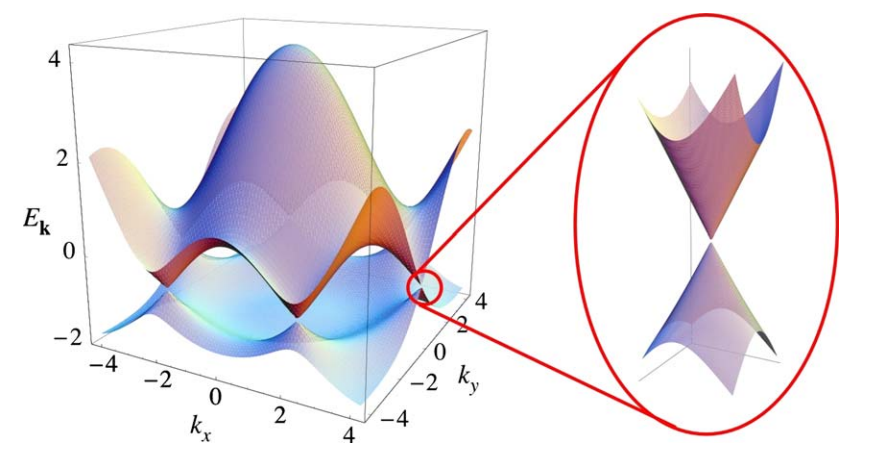
\includegraphics[width=0.6\textwidth]{images/background/ElecPropertiesFig3.png}
    \caption[The band structure of graphene]{The band structure of graphene. At the corners of the Brillouin zone the upper and lower bands meet. Near these points, known as Dirac points, the dispersion relation is approximately linear. Adapted from \cite{CastroNeto2009}.}
    \label{fig:bandstructure}
    \end{figure}


	\subsection{Dirac fermions}
    In the low energy regions near the corners of the Brillouin zone the dispersion relation for graphene is approximately linear, as indicated in Figure \ref{fig:bandstructure}. That is, for electrons or holes near these points,
    \begin{equation}
    E = \hbar v_F \sqrt{k_x^2 + k_y^2}
    \end{equation}
    (where $k_x$ and $k_y$ are measured from the corner point). This has the same form as the energy of a massless, relativistic particle governed by the Dirac equation. These points are therefore called Dirac points, and in their vicinity the electrons behave as massless Dirac fermions. Each corner of the hexagonal Brillouin zone is related to two others by a reciprocal lattice vector, therefore two of the Dirac points, typically labelled $K$ and $K'$ are inequivalent.

    The linear dispersion relation is not the only factor which ties transport in graphene to the Dirac equation; the two-component wavefunction of pseudoparticles in graphene is analogous to the spinor wavefunction used to describe spin $\frac{1}{2}$ particles in the Dirac equation \cite{Katsnelson2006}. In graphene the two components correspond to the contributions to the pseudoparticle wavefunction from each of the two sublattices, whereas in quantum electrodynamics (QED) the spinor accounts for the spin up and spin down components of the wavefunction.

	\subsection{Quantum Hall effect}
    Graphene displays a unique variant of the quantum Hall effect due to the massless, 
    Dirac fermion nature of its charge carriers \cite{Novoselov2005}, \cite{Zhang2005}. In fact,
    the observation of graphene's alternative manifestation of the quantum Hall effect provided
    one of the first experimental confirmations of the nature of charge carriers in graphene.
    In order to better emphasize the uniqueness of the quantum Hall effect
    in graphene we begin with a description of the standard quantum Hall effect.
    
    In typical two-dimensional materials the application of a large magnetic 
    field leads to a quantization of the allowed energy levels. These quantized energy states are 
    called Landau levels, and for massive carriers the allowed energies are given by
    \begin{equation}
        E=\hbar \omega_c (n + 1/2) \;\;\; \text{with} \;\;\; \omega_c = \frac{e B}{m^*}.
    \end{equation}
    The conductivity of a two-dimensional device in a high magnetic field depends on the location of the Fermi level
    relative to these Landau level energy states.
    
    slight digression: experimentally what is measured in both the lateral and longitudinal case is the 
    voltage between two contacts.
    \note{why this gives conductivity in one direction, resistivity in the other}
    
    \note{understand this better}
    When the Fermi level coincides with one of the allowed Landau level energies the longitudinal 
    resistivity $\rho_{xx}$ displays a peak.
    Additionally, the lateral Hall conductivity $\sigma_{xy}$ will increase by $4 e^2/h$.
    When the Fermi level lies between the allowed energy levels the longitudinal resistivity goes to 0,
    and the Hall conductivity remains constant.
    
    These features are most readily observed by sweeping the Fermi level through successive Landau
    level states, which can be accomplished by varying either the applied magnetic field
    or the carrier density. In the former case the Fermi level remains fixed while the allowed Landau level energies
    vary, while in the latter case the Fermi level is varied and the Landau level energies are constant.
    
    which when successively filled by 
    increasing the carrier concentration yield plateaux in the Hall conductivity at 
    $\sigma_{xy} = \pm (4e^2/h) N$ where $N$ is an integer. Additionally, in typical materials 
    there is no Landau level at $E=0$, due to the 
    quantization of massive particles in a magnetic field, therefore the first plateaux 
    appear at $\pm 4 e^2/h$. 
    
    The quantum Hall effect as observed in graphene differs from the 
    standard, integer QHE in two ways: the plateaux are shifted by $2 e^2/h$ and the sequence 
    is uninterrupted as it passes through zero carrier density. Both differences stem from 
    the massless character of graphene's charge carriers.

    , as seen in Figure \ref{fig:QHEinG}. 
    
    For massless particles in a magnetic field, such as the Dirac fermions in graphene, the energy quantization is $E = [ 2 e \hbar {c\ast}^2 B (N + 1/2 \pm 1/2) ]^{1/2}$ \cite{Novoselov2005}, where the sign of the last term depends on the pseudospin (or sublattice index) of the particle. This has two consequences; first, when $\pm \rightarrow -$ this quantization admits an $E=0$ Landau level, which in turn causes the sequence of plateaux in the Hall conductivity to be uninterrupted as it passes through zero carrier density. Second, the $E=0$ Landau level admits only those particles with `minus' pseudospin polarization, therefore it is half as degenerate as all other LLs. This accounts for the $1/2$ offset in the locations of the Hall conductivity plateaux in graphene, $\sigma_{xy} = (4 e^2/h )(N + 1/2)$.

    An additional consequence of the masslessness of charge carriers in graphene is the persistence of quantum Hall effects to room temperature \cite{Novoselov2007}. Considering again the energy quantization for Dirac fermions in a magnetic field quoted above, for $c\ast = v_F \approx 10^6$ m $s^{-1}$ a 45 T field yields an energy gap of $\approx$ 2400 K between the $N=0$ and $N=\pm1$ Landau levels, an order of magnitude greater than thermal fluctuations at room temperature. The high carrier concentration and temperature-independent carrier mobility also contribute to the robustness of the effect \cite{Novoselov2007}.

    \begin{figure}
    \centering
    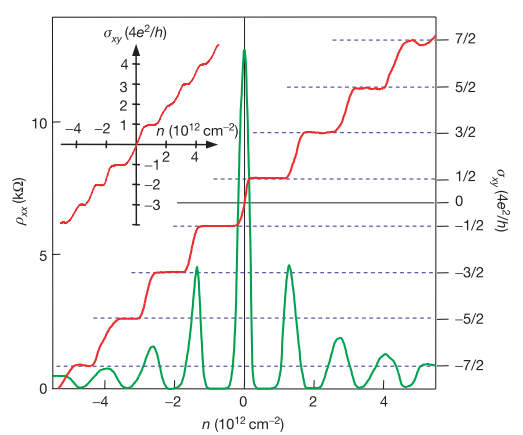
\includegraphics[width=0.45\textwidth]{images/background/QHEinG.png}
    \caption[The quantum Hall effect in graphene]{The quantum Hall effect in graphene. The Hall conductivity and longitudinal resistivity are plotted as a function of carrier concentration. Hall plateaux are present at $4 e^2 / h (N + 1/2)$, offset from the expected values by $2 e^2 / h$, and continue uninterrupted through zero concentration. Inset: Hall conductivity versus carrier concentration for bilayer graphene, showing the expected characteristics of the integer quantum Hall effect for comparison. Adapted from \cite{Novoselov2005}.}
    \label{fig:QHEinG}
    \end{figure}

        
    \section{Doping graphene}
    
        \subsection{Electrostatic gating}
        
        \subsection{Chemical adsorbates}
    
        \subsection{Substrate effects in graphene}
        The substrate used to support graphene strongly affects electrical transport in the graphene. Scattering by surface phonons at the SiO$_2$ interface has been shown to limit the room temperature mobility of graphene \cite{Chen2008}, and scattering by charge impurities is responsible for the asymmetry between electron and hole conductivities \cite{Hwang2007}. Charge impurities can also create inhomogeneities in graphene's local carrier density, which are thought to be responsible for the saturation of conductivity at low carrier densities \cite{Hwang2007}. Substrate features can also cause delamination of the graphene from the substrate; previous work has observed a snap-through transition for multilayer graphene on corrugated substrates \cite{Scharfenberg2012} as well as the formation of network of wrinkle delaminations on a substrate decorated with silica nanoparticles \cite{Yamamoto2012}.
    
        Certain experiments, in an attempt to minimize the effect of the substrate have fabricated devices using suspended graphene \cite{Bolotin2008}, \cite{Du2008}. In a particularly noteworthy example, the authors of ref \cite{Bolotin2008} observed carrier mobilities of up to 200,000 cm$^2$ V$^{-1}$ s$^{-1}$, an order of magnitude greater than the best results for graphene on silicon substrates, showing that the substrate can have a distinct impact on graphene's electrical properties. Recently several groups have also begun fabricating graphene devices on hexagonal boron nitrides (hBN) substrates, where the atomically flat surface, large bandgap, and similar lattice constant to graphene yield drastically improved electronic properties compared to samples fabricated on SiO$_2$ substrates \cite {Dean2010}, \cite{Xue2011}.
    
        Alternatively, strong substrate interactions can also be used to deliberately tune graphene's electrical properties. In particular, functional ferroelectric substrates such as PbZr$_{0.2}$Ti$_{0.8}$O$_3$ (PZT) have been shown to vary carrier type and density in graphene with varying substrate polarizations \cite{Baeumer2013}, as seen in Figure \ref{fig:GonPZT}. This effect is bidirectional: application of a large bias to the graphene can also flip the polarization of the underlying PZT.
    
            %\begin{wrapfigure}[25]{R}{0.50\textwidth}
            \begin{figure}
            \centering
            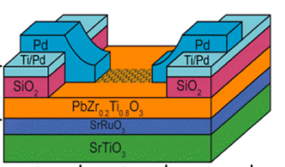
\includegraphics[width=0.35\textwidth]{images/background/ChristophDevice.png}
            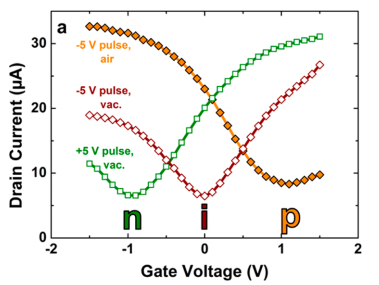
\includegraphics[width=0.45\textwidth]{images/background/ChristophFig4.png}
            \caption[Graphene on ferroelectric substrates]{Left: A graphene FET fabricated on a PZT substrate. Right: Variable carrier type in a graphene FET on a ferroelectric substrate. I-V sweeps are shown for for the same device after gate voltage pulses are applied to switch the polarization of the ferroelectric layer. Adapted from \cite{Baeumer2013}.}
            \label{fig:GonPZT}
            \end{figure}
        
        
    \section{Straining graphene}
    
        \subsection{Graphene's mechanical strength}
    
        \subsection{Band gap engineering}
        Several research groups have considered, both experimentally \cite{Ni2008}, \cite{Kim2009}, \cite{Mohiuddin2009}, \cite{Zang2013} and theoretically \cite{Pereira2009}, \cite{Low2011}, the effect of uniaxial strain on graphene. A number of results are consistent between groups. First, the effect of uniaxial strain on the electronic properties of graphene can be observed through Raman spectroscopy; in ref \cite{Ni2008} the authors observe shifts in the G and 2D band peaks of -27.8 and -14.2 cm$^{-1}$ / percent strain respectively, confirming the interactivity of strain and graphene's electronic properties as well as offering a method to locally measure the strain applied to graphene.
    
        Second, uniaxial strain is predicted to open a gap in the band structure, either by itself at high strains \cite{Pereira2009} or in conjunction with a correlated scalar potential \cite{Low2011}. Experimental work following the latter approach observed an increasing sheet resistivity with decreasing temperature in a graphene device patterned atop lithographically defined corrugations on a SiO$_2$ substrate \cite{Lee2013}. This behavior is indicative of a gap in the band structure, which the authors calculate to be approximately 200 meV. In this case the periodic potential comes from the periodic, substrate-induced doping in the regions not covered by the corrugations.
    
        \subsection{Pseudomagnetic fields}
        Recent work, both theoretical \cite{Guinea2009} and experimental \cite{Levy2010}, \cite{Yan2012} suggests that non-uniform strains in graphene have an effect similar to an applied magnetic field. From a theoretical perspective these strain-induced pseudomagnetic fields stem from a modification of the nearest and next nearest neighbor hopping amplitudes; as the lattice is strained the distances between lattice sites vary, and with them the relevant hopping amplitudes $t$ and $t'$. This strain effect can be modeled by introducing a gauge field vector potential, which has an effect similar to that of a magnetic vector potential field. However, unlike an actual magnetic field a strain-generated pseudomagnetic field has a different sign for charge carriers in the \textbf{K} and \textbf{K'} Dirac points, and therefore does not violate time reversal symmetry \cite{Guinea2009}.
    
        These pseudomagnetic fields are predicted to be on the order of tens of tesla. Such high fields, in conjunction with graphene's high carrier concentration and mobility, offer the potential to observe a zero field quantum Hall effect. A key requirement in generating pseudomagnetic fields is that the strain profile be anisotropic; to date experimental efforts have focused on strain created by nanobubble \cite{Levy2010} or nanoridge \cite{Yan2012} defects. However defect-oriented experimental design schemes yield extremely small areas of graphene under strain, and as such the strain-related physics is only accessible through scanning tunneling microscopy (STM) measurements. Therefore in order to observe macroscopic transport effects like a zero field quantum Hall effect I propose a device scheme with arrays of patterned strain-inducing features.



\chapter{Experimental Techniques}

    This thesis describes the results of experimental work, and while the experimental results comprise the bulk
    of this work's novelty a thorough record of the the experimental methods employed to produce those results 
    is crucial for future reproducibility.
    In this chapter I present a summary of the fabrication, characterization, and measurement techniques used
    in the course of this research.
    
    \section{Sample Fabrication}
    
        Sample fabrication is the primary task for experimental work on graphene devices, 
        and can broadly be divided into two subtasks: producing graphene and shaping it into useful geometries.
        In this section I present the experimental techniques used to produce graphene
        and shape it into devices appropriate for optical and electrical transport measurements.
    
        \subsection{Graphene synthesis and transfer}
        
        
            \subsubsection{Mechanical exfoliation}
            
            There are two widely used methods used to produce graphene for 
        experimental research: mechanical exfoliation\cite{novoselov2004electric} and chemical vapor
        deposition (CVD) growth\cite{li2009large}. In mechanical exfoliation highly ordered
        pyrolitic graphite is repeatedly cleaved, typically by attaching and 
        then peeling off Scotch tape. After a succession of such cleaving steps
        small regions of monolayer graphene are left attached to the Scotch
        tape, which are then transferred to a silicon wafer having a 300nm
        thick layer of SiO$_2$. An optical interference effect caused by the 
        combination of the oxide layer and the graphene allows the graphene
        regions to be identified with an optical microscope \cite{Blake2007}.
        This process is illustrated schematically in Figure \ref{fig:exfoliation}.
        Mechanical exfoliation produces the highest quality graphene as
        measured by electron mobility; values up to 60,000 cm$^2$ V$^{-1}$
        s$^{-1}$ have been reported \cite{Dean2010}. However, the size of the 
        resulting graphene flakes is limited, typically to tens of square
        microns, and the transfer process precludes any alignment of graphene
        with pre-existing substrate features.
        
            \begin{figure}
            \centering
            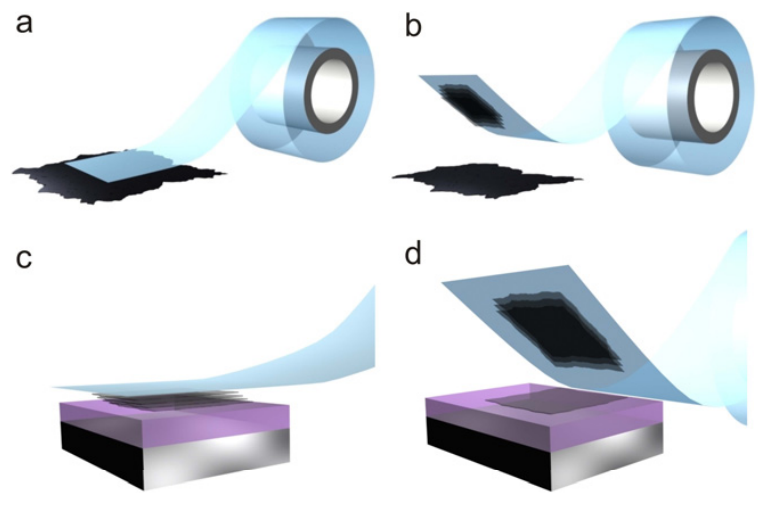
\includegraphics[width=0.6\linewidth]{images/experimentaltechniques/exfoliation.png}
            \caption[Mechanical exfoliation of graphene]{
                \textbf{(a-b)} Highly ordered pyrolitic graphite is cleaved using Scotch tape.
                \textbf{(c)} The cleaved graphite is pressed onto the target substrate.
                \textbf{(d)} The Scotch tape is peeled off the target substrate, leaving a monolayer of graphene.
                Image adapted from \cite{novoselov2012two}}
            \label{fig:exfoliation}
            \end{figure}

        
            \subsubsection{CVD growth}

            In the CVD growth process a metal foil, usually nickel or copper, is
        placed in a vacuum furnace and heated while H$_2$ and CH$_4$ are 
        introduced at controlled rates and for controlled times. Properly
        optimized growth recipes will yield uniform, monolayer graphene on
        top of the metal foil \cite{reina2008large, kim2009large, li2009large, li2009transfer}. 
        For the precise recipes used to grow the graphene used in this research see Appendix \ref{appendix:fab}.
        
        Unlike graphene produced by mechanical
        exfoliation, CVD graphene usually (though not always, see 
        \cite{Petrone2012}) has multiple domains \cite{Li2010} which accounts
        for its lower quality, again as measured by electron mobility. Typical
        values for CVD graphene are in the $10^3$ to $10^4$ cm$^2$ V$^{-1}$
        s$^{-1}$ range \cite{Petrone2012}. From a practical perspective, the 
        disadvantage of CVD graphene's limited mobility
        is counter-balanced by the ease and volume of production via this method:
        while exfoliated graphene flakes are limited to tens of square microns, 
        CVD graphene has been grown in 30 inch-wide films\cite{bae2010roll}.
        Larger graphene films allow for entire substrates to be covered, which 
        in turn allows for device designs where graphene is deposited atop existing
        substrate features.
        
            \subsubsection{Wet transfer}
            
            Graphene grown on metal foils by chemical vapor deposition must be transferred to 
        an insulating substrate before its electrical properties can be measured.
        This transfer is a critical step: if done poorly it has the potential to 
        drastically alter the properties of the graphene, whether by destroying
        the mechanical integrity of the graphene or by introducing substantial electrical doping.
        Transferring graphene onto flexible or patterned substrates introduces additional
        complexities. 
        
        \begin{figure}
            \centering
            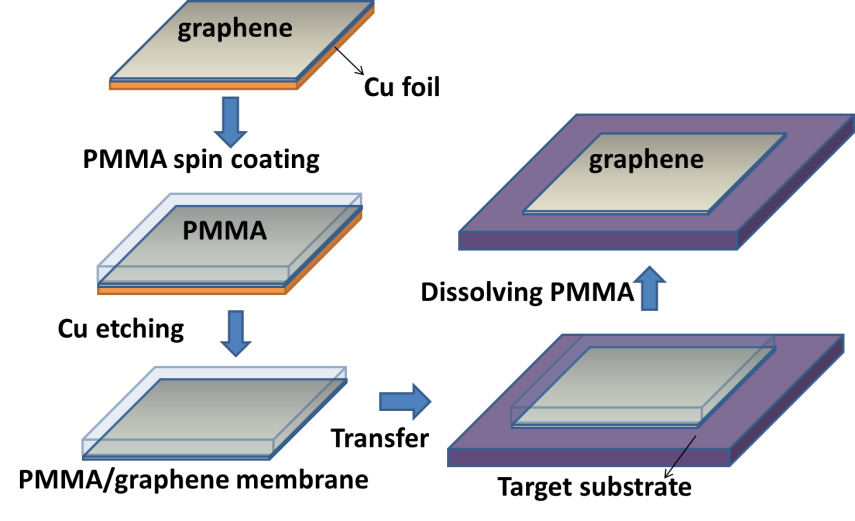
\includegraphics[width=0.8\linewidth]{images/experimentaltechniques/wettransfer.png}
            \caption[Wet transfer of CVD graphene]{
                `Wet transfer' of CVD graphene.
                Image adapted from \cite{kumar2013synthesis}}
            \label{fig:wettransfer}
        \end{figure}

        The simplest transfer procedure is illustrated schematically in Figure \ref{fig:wettransfer} \cite{reina2008large, kim2009large, li2009large}.
        Copper foil with CVD graphene grown on top is coated with a thin, sacrifical layer of the 
        polymer poly(methyl methacrylate) (PMMA) and then placed in a bath of 0.1M ammonium persulfate
        to etch away the metal. Once the metal is removed the PMMA-coated graphene 
        remains floating on the surface of the solution. The ammonium persulfate solution is then flushed and replaced
        with de-ionized water.
        Finally the floating graphene / PMMA stack can be
        scooped onto the desired substrate, at which point the PMMA is removed using acetone.
        
        This process is delicate, and in practice the quality of the transfer depends on several 
        analog factors. First, the ammonium persulfate solution must be thoroughly replaced by de-ionized water;
        if traces of the original solution remain when the graphene is transferred to the target substrate
        then redeposited copper residue will be present between the graphene and the target substrate upon drying. 
        Figure \ref{fig:bad_xfer_cu} shows a substrate contaminated by redeposited copper after graphene transfer.
        Second, the angle of the substrate relative to the surface during the scooping step must be close
        to ninety degress. If the graphene is scooped at a shallow angle the graphene will trap a bubble of water
        beneath itself; as the water evaporates the graphene will wrinkle.
        
         \begin{figure}
            \centering
            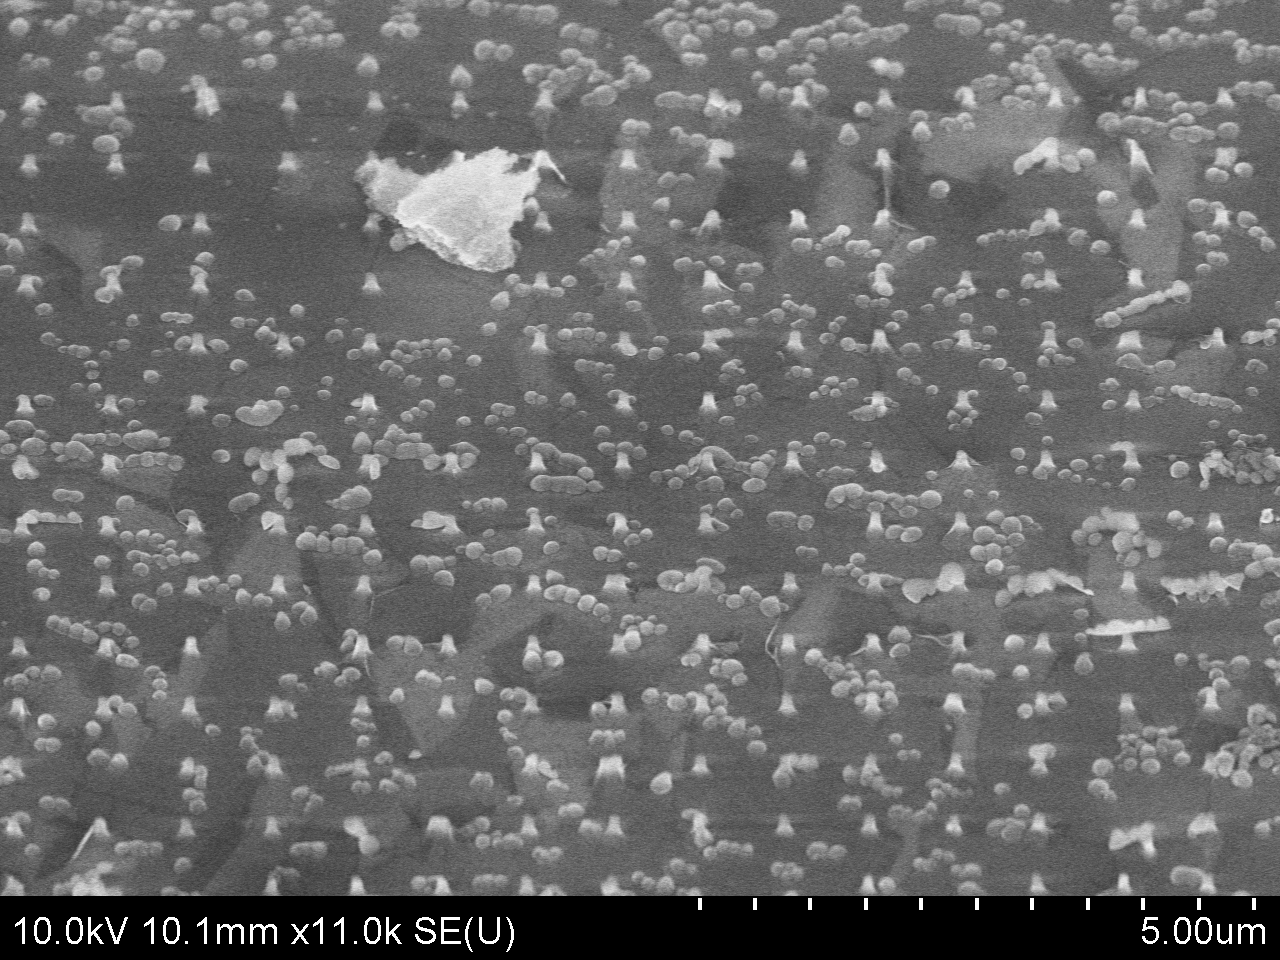
\includegraphics[width=0.4\linewidth]{images/experimentaltechniques/bad_xfer_cu.png}
            \caption[Copper contamination from bad graphene transfer]{
                SEM micrograph of a substrate contaminated by redeposited copper as a result of 
                imcomplete removal of the ammonium persulfate solution. The round debris are 
                the copper; the regularly spaced pillars are the result of deliberate fabrication.
            }
            \label{fig:bad_xfer_cu}
        \end{figure}


            \subsubsection{Copper transfer}
            
        The standard wet transfer procedure fails in cases where the graphene must be 
        transferred to polymer substrates: the final acetone step which removes the sacrificial
        PMMA layer also damages the target substrate.
        In this case the transfer can be accomplished using a two-part process as illustrated in
        Figure \ref{fig:cutransfer} and adapted from \cite{Lee2010}. First, using the standard wet transfer process
        graphene is transferred to an intermediate substrate coated in a thin layer of copper. Next the 
        target substrate is mechanically pressed onto the intermediate substrate. The two substrates
        are then immersed in a chemical bath which etches the copper layer, leaving the graphene
        attached to the target, polymer substrate.
        
        This transfer procedure also allows the creation of patterned graphene devices on polymer substrates.
        Typical lithographic processes do not work with flexible substrates, however when using this
        copper transfer procedure the graphene can be patterned on the rigid intermediate substrate. The
        final transfer onto the target substrate then produces patterned graphene on a flexible substrate.
            
            \subsubsection{Critical point drying transfer}
            
        Substrates having topographic features present another complication when transferring graphene.
        For such substrates the graphene will delaminate from the substrate in the vicinity of the 
        vertical substrate features. When the sample is allowed to dry
        after the removal of the sacrificial PMMA layer, the surface tension of the evaporating solvent will tear
        the suspended graphene. Figure \ref{fig:cpdtear} shows a scanning electron microscope microgram of 
        graphene torn by this mechanism.
        
        \begin{figure}
            \centering
            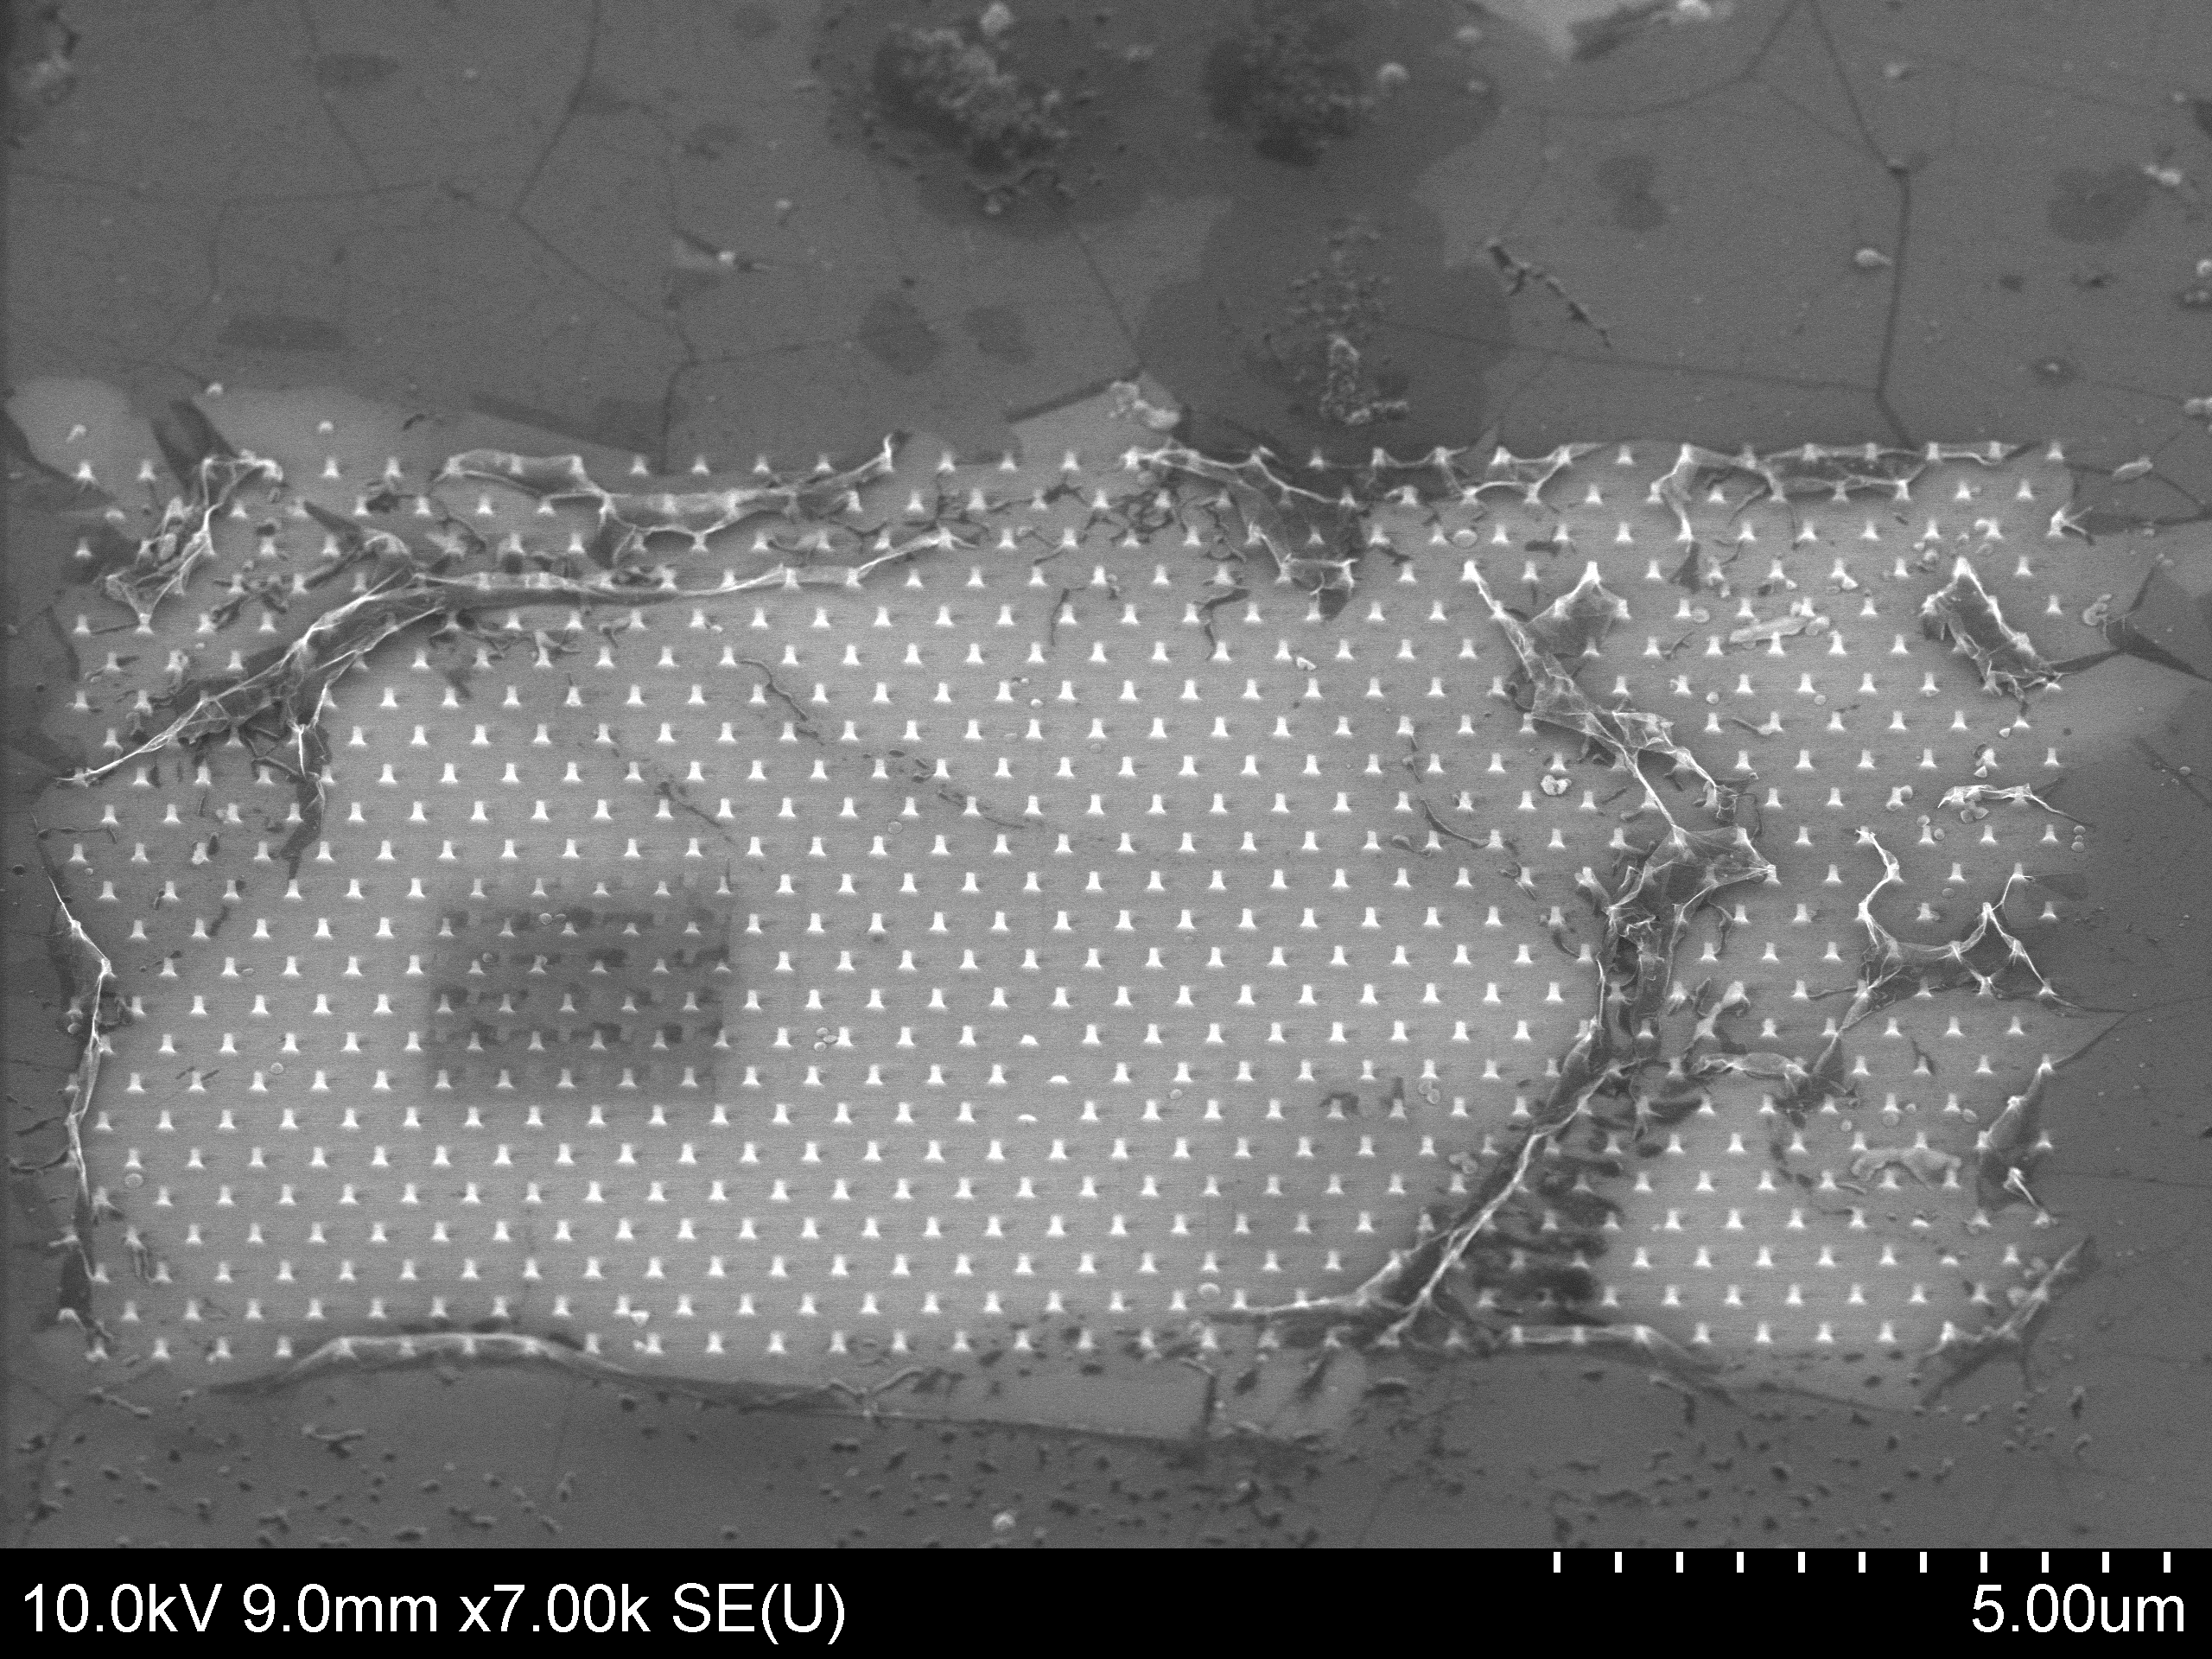
\includegraphics[width=0.5\linewidth]{images/experimentaltechniques/cpdtear.png}
            \caption[Graphene tears from solvent surface tension]{
                Graphene ripped in the vicinity of an array of pillars. The graphene 
                was ripped by the surface tension
                of evaporating solvents. The dark rectangle in the middle of the ripped region
                is an artifact of surface charging from a previous SEM scan.
                }
            \label{fig:cpdtear}
        \end{figure}

        The damaging effect of the evaporating solvent can be mitigated by performing the final
        drying step in a critical point drying apparatus. In this procedure graphene
        is transferred to the target substrate using the standard wet transfer process. 
        However after the 
        final acetone step to remove the sacrificial PMMA the substrate is transferred
        to the chamber of a critical point drying machine while still in liquid.
        The chamber is sealed, liquid CO$_2$ is introduced, and then the chamber is heated until the environment 
        reaches a super-critical phase. The chamber is flushed while in the super-critical state,
        then depressurized, thereby drying the sample without ever exposing the suspended graphene 
        to the surface tension of evaporating solvents.
            
            
        \subsection{Substrate patterning}
        
            \subsubsection{Lithography}
            
            Once transferred to the desired substrate, graphene must be shaped into geometries
            appropriate for measurements and contacted with metal leads; for both tasks the 
            required patterns are defined using either photo- or electron-beam lithography.
            Similarly, for devices where the substrate is modified lithography is used to
            define the required profiles.
            Lithography is a standard experimental technique, and as such a complete description
            of the principles behind its operation lies outside the scope of this thesis. However,
            certain aspects of the fabrication used in this research required
            slight modifications to established lithography procedures. These modifications
            are described conceptually below, for the exact processes used see Appendix \ref{appendix:fab}.
            
            First, the flexible substrates used in this research are not amenable to standard lithography. 
            In order to produce graphene devices on such substrates the graphene must be patterned
            prior to being transferred to the flexible substrate. The copper transfer procedure
            described above allows for this: after the first transfer step the graphene 
            can be patterned while on the intermediate, copper coated substrate. Once the graphene
            is patterned the transfer process is completed, yielding patterned graphene on a flexible 
            substrate.
            
            Second, devices having suspended graphene (like those produced by the critical point
            drying method described above) present an additional challenge: once graphene is freely
            suspended on the substrate no further patterning can be done because applying a new layer
            of resist will destroy the graphene. To circumvent this issue we pattern the graphene
            before it becomes free standing by using the same PMMA layer
            used to transfer the graphene as a resist layer during an electron beam lithography step.
            
            \subsubsection{Deposition}
            
            A substantial fraction of the results in this thesis are the result of electrical transport measurements.
            Performing transport measurements on graphene requires robust electrical contact between
            graphene and the measurement apparatus; this contact is created by depositing
            metal leads atop the graphene using an electron beam evaporator. 
            Metal deposition using an electron beam evaporator is also a standard experimental technique
            so we again omit a detailed description of the technique.
            For the devices described here we use gold leads along with a sticking layer made of either
            titanium or chromium; for the exact deposition recipes used see Appendix \ref{appendix:fab}.
            
            \subsubsection{Reactive ion etching}
            
            Reactive ion etching (RIE) is the primary subtractive patterning technique used 
            to fabricate our devices. We use RIE for two particular patterning tasks: first, to 
            shape uniform sheets of CVD graphene into device geometries, and second to etch
            topographic features into SiO$_2$ substrates. 
            Each etching task requires an appropriate chemistry; for graphene etching we use
            an O$_2$ plasma and for SiO$_2$ etching we use CHF$_3$.
            For the exact RIE processes used in this work see Appendix \ref{appendix:fab}.
    
    \section{Sample Characterization}
    
    The primary challenge of experimental condensed matter research, at least as measured by graduate student effort, lies in fabricating working devices. The fabrication techniques described above require finesse, skill, and a certain degree of luck (especially when working with temperamental equipment). As such, a substantial fraction of the fabricated devices will fail to work. Characterizing the different failure modes of a given fabrication process -- and thereby determining the optimal process parameters -- is a crucial part of each research project. In this section several techniques which effectively characterize the quality and physical integrity of graphene and other fabricated device elements are described.
    
        \subsection{Atomic Force Microscopy}
        
        Atomic force microscopy (AFM) measurements offer an excellent way to verify the mechanical integrity
        of graphene. A complete description of the principles underlying the operation of an AFM lies beyond
        the scope of this thesis; here we offer a brief description of several of the primary modes of 
        atomic force microscope operation which are used in this research.
        Atomic force microscopes can be operated in two primary modes: tapping and contact.
        In contact mode a sharp tip mounted on a cantilever is dragged across a surface, and the 
        topography of the surface is measured by observing the deflection of a laser reflected off of the cantilever.
        Tapping mode proceeds similarly, however the tip is raised slightly above the surface and oscillated.
        In this mode both the amplitude and phase (relative to the driving force) of the tip's oscillation are measured.
        
        Phase measurements in tapping mode (i.e. measurements of the phase between the drive
        and response of an oscillating AFM tip) are particularly sensitive to the interaction of the AFM tip and 
        the substrate. This sensitivity produces a high contrast in measurements that scan across two different materials,
        for example graphene and SiO$_2$. This contrast in turn makes it easy to observe rips in graphene
        and thereby investigate its mechanical integrity. Figure \ref{fig:afm_rips} illustrates this high contrast.
        
         \begin{figure}
            \centering
            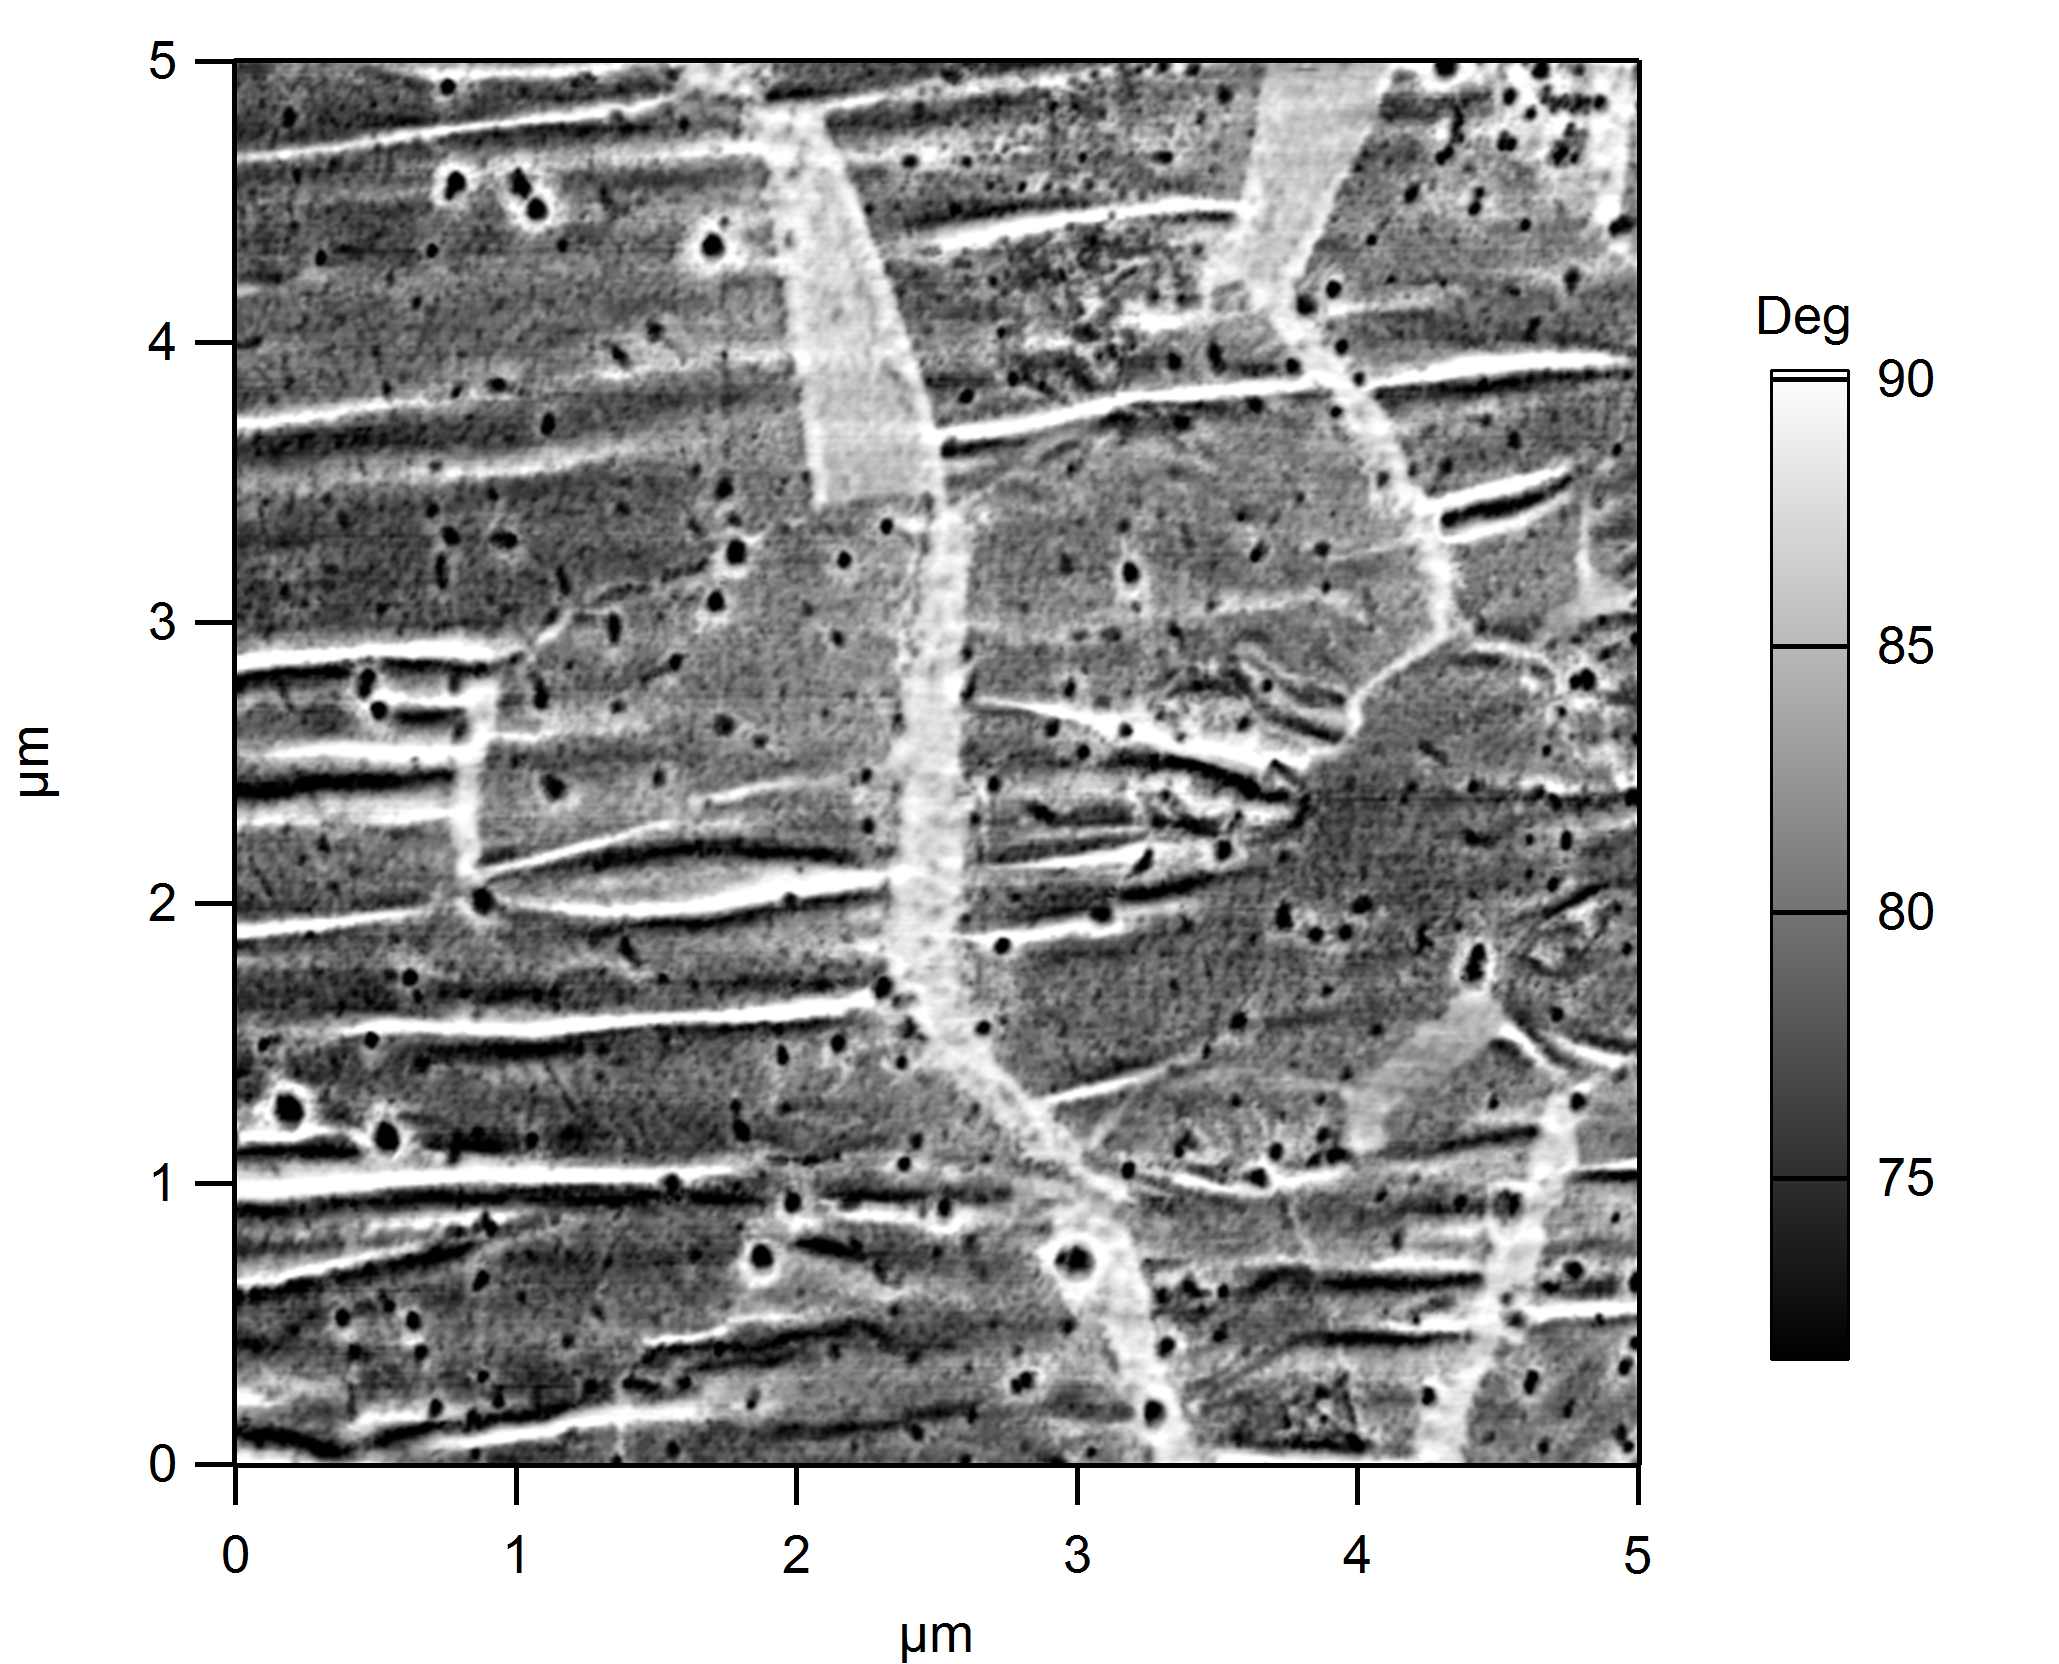
\includegraphics[width=0.5\linewidth]{images/experimentaltechniques/AFMrips.png}
            \caption[AFM micrograph of ripped graphene]{
                AFM phase measurements of ripped graphene on a PDMS substrate. The vertical, light-colored
                features are rips in the graphene; the high contrast is due to the different tip 
                interaction on the graphene compared to the PDMS. Horizontal features are wrinkles
                in the graphene.
                }
            \label{fig:afm_rips}
        \end{figure}
       
        Conductive AFM tips enable a secondary set of measurement modes which probe electrical properties of the sample.
        In piezoresponse force microscopy (PFM) mode, an AFM tip is placed in contact with the substrate
        and an AC bias is applied to the tip. For ferroelectric substrates the applied voltage
        will create a deformation in the substrate which can be measured by the deflection of the AFM cantilever. 
        The deformation is proportional to the ferroelectric polarization; in particular opposite polarizations in the substrate
        will reverse the direction of the deformation, thereby changing the relative phase between the driving AC bias
        and the observed response by a factor of $\pi$. By measuring the phase one can therefore measure
        the polarization of the substrate. 
        
        Conductive AFM tips can also be used to `write' polarization domains in ferroelectic substrates.
        In this mode, a bias above the conducive voltage of the ferroelectric material is applied to the tip 
        during a contact-mode scan. As the tip is scanned across the substrate the local voltage applied by the 
        tip bias flips the substrate polarization and establishes a domain.
        Examples of PFM measurements and domain writing are shown in Figure \ref{fig:PFM_example}.
        
        \begin{figure}
        \centering
        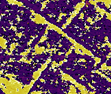
\includegraphics[width=0.25\textwidth,height=0.225\textwidth]{images/experimentaltechniques/PFM-1.png}\hspace{0.05\textwidth}
        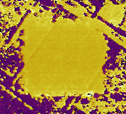
\includegraphics[width=0.25\textwidth]{images/experimentaltechniques/PFM-2.png}\hspace{0.05\textwidth}
        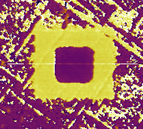
\includegraphics[width=0.25\textwidth]{images/experimentaltechniques/PFM-3.png}
        \caption[PFM micrographs of ferrelectric domains in PZT]{PFM phase images of a PZT substrate. Left: as grown, in a
                 polydomain configuration. Center: after writing a `poled down' domain
                 with a negatively biased AFM tip in contact mode. Right: after writing a
                 smaller `poled up' domain with a positively biased AFM tip. The `poled down'
                 domain is approximately 5 microns wide.}
        \label{fig:PFM_example}
        \end{figure}
        
        
        Kelvin probe force microscopy is an AFM mode which probes the surface potential of a substrate.
        In KPFM mode, a conductive AFM tip is placed a constant distance above the substrate
        and an AC bias is applied to the tip. In this configuration the AFM tip and the substrate form a capacitor.
        The energy stored in a capacitor is proportional to the potential difference across the capacitor, 
        which in this case is a function of both the applied AC bias and any DC offset between the tip and the substrate.
        If the AC bias is applied at the resonant frequency of the AFM cantilever the energy takes the form
        \begin{equation}
        E = \frac{1}{2}C[V_{DC} + V_{AC}\sin(\omega_0 t)]^2 = \frac{1}{2}C[2V_{DC}V_{AC}\sin(\omega_0 t) - \frac{1}{2}V_{AC}^2 \cos(2\omega_0 t)]
        \end{equation}
        In this case the force on the cantilever (and thus the measured response) at the cantilever's resonant 
        frequency is proportional to the DC offset between the tip and the substrate. By scanning the tip across
        the substrate at a constant separation and observing the change in oscillation amplitude 
        the potential difference between the tip and the substrate, and thereby
        the work function can be mapped over the whole substrate.
        
        AFM measurements are well suited to flat sample geometries. For samples with topographic features
        however the measurements are limited by the sharpness of the AFM tip: AFM measurements are a convolution
        of the AFM tip shape and the substrate shape, and when the substrate is sharper than the AFM tip the finer details
        of the measurement will be washed out.
        This limitation is especially apparent on samples which have very sharp topographic features.
        
        \subsection{Scanning Electron Microscopy}
        
        Scanning electron microscopy (SEM) is another useful characterization tool, especially for samples
        which have very sharp topographic features. SEM is a standard experimental technique and does
        not require any special adaptations for the devices described in this thesis, and so will
        not be described in detail here.
        
        \subsection{Raman Spectroscopy}
        
        Raman spectroscopy is another characterization technique which is particularly useful for
        its ability to non-intrusively measure certain electrical properties of graphene.
        Pristine graphene has a well characterized Raman signature \cite{ferrari2006raman}, and deviations
        from this signature can be used to measure the quality of the graphene.
        Two features in graphene's Raman signature are particularly relevant: first, the presence of a 
        Raman peak near 1350 cm$^{-1}$ (referred to as the D peak) indicates that there are defects present in the graphene lattice
        which will reduce the electrical quality of the graphene. Second, the shapes and relative magnitudes
        of the Raman peaks at 1590 cm$^{-1}$ and 2600 cm$^{-1}$ (referred to as the G and 2D peaks, respectively)
        can be used to determine the number of graphene layers present in the sample: for high quality
        monolayer graphene the 2D peak should have a greater intensity than the G peak, and both peaks
        should be well approximated by a Lorentzian distribution. Figure \ref{fig:pristine_raman}
        shows the change in the shape of the 2D peak with increasing graphene thickness.
        
        \begin{figure}
            \centering
            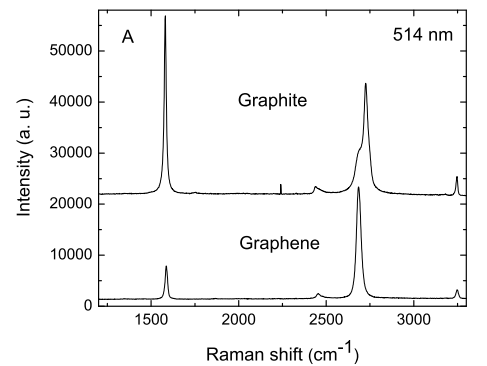
\includegraphics[width=0.49\linewidth]{images/experimentaltechniques/pristine_raman_2.png}
            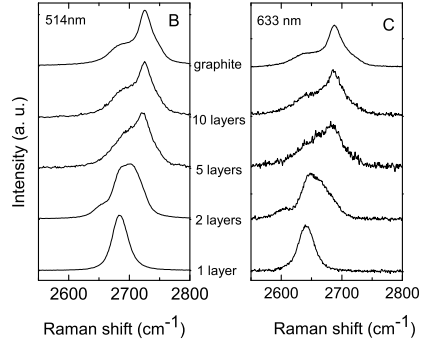
\includegraphics[width=0.49\linewidth]{images/experimentaltechniques/pristine_raman_1.png}
            \caption[Raman spectra of graphene]{
                Raman spectra of mono- and multilayer graphene. As the number of layers increases the G peak
                (at 1600 cm$^{-1}$) intensity increases relative to the 2D peak (at 2700 cm$^{-1}$) and the 
                shape of the 2D peak deviates from a Lorentzian.
                Adapted from \cite{ferrari2006raman}.
                }
            \label{fig:pristine_raman}
        \end{figure}
        
        Raman measurements of graphene can also be used to gain information about the electrical doping
        and strain present in graphene \cite{lee2012optical}. Both strain and doping produce shifts
        in the G and 2D peak locations by modifying the bond lengths in the graphene lattice. 
        A measurement of either peak shift by itself is therefore insufficient to disentangle the competing effects
        of strain and doping. However, the two mechanisms (strain and doping) shift the locations of the two
        peaks by different relative amounts; the ratio
        $$
        r = \frac{\Delta \omega_{2D}}{\Delta \omega_G}
        $$
        where $\Delta \omega$ is the shift in the specified Raman peak, differs between the two mechanisms \cite{lee2012optical}.
        Experimental measurements \cite{zabel2012raman, metzger2009biaxial, ding2010stretchable} and theoretical \cite{mohr2010splitting, mohiuddin2009uniaxial} results place the ratio for strain between 2.25 and 2.8 and the ratio for doping at approximately 0.75 \cite{lee2012optical}.
        Thus by plotting the Raman G and 2D peak positions against one another and comparing to the expected
        values for intrinsic, unstrained graphene one can decompose the peak shifts into components due to
        strain and doping\cite{lee2012optical}. This decomposition is shown in Figure \ref{fig:raman_decomposition}.
        
        \begin{figure}
            \centering
            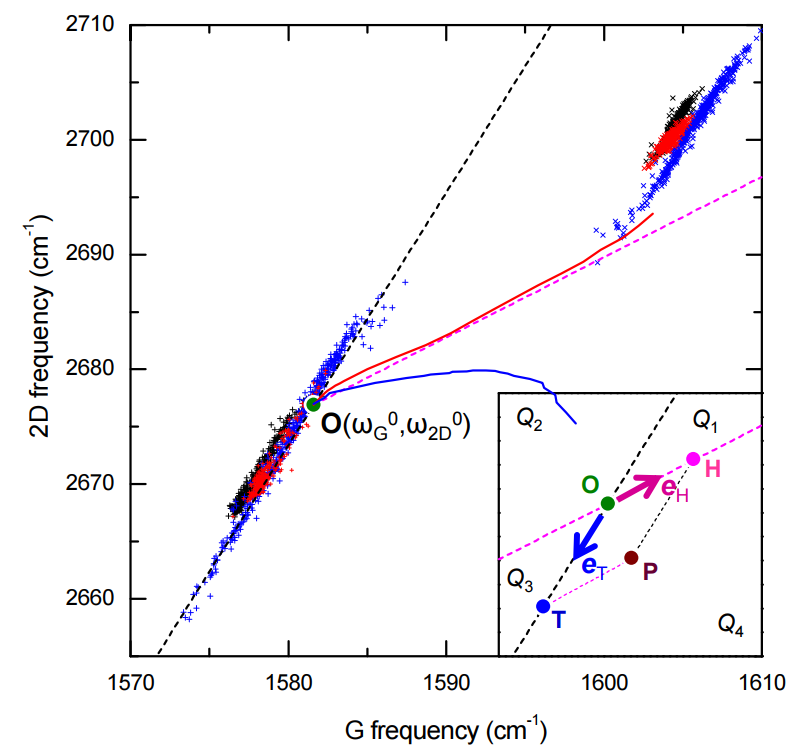
\includegraphics[width=0.5\linewidth]{images/experimentaltechniques/lee2012_raman.png}
            \caption[Graphene G vs 2D peak positions for strain and doping]{
                Raman G and 2D peak locations for graphene.
                The black dashed line shows the ratio 
                $r = \frac{\Delta \, \omega_\text{2D}}{\Delta \, \omega_\text{G}}$ expected for shifts due to
                strain, and the purple dashed line shows the ratio expected for shifts due to doping.
                The two lines intersect at the expected peak positions for undoped, unstrained graphene.
                By comparing measured Raman G and 2D peak positions to vectors corresponding to the
                black and purple lines one can determine the degree to which strain and doping, respectively,
                contribute to the observed shifts in peak positions.
                Adapted from \cite{lee2012optical}.
                }
            \label{fig:raman_decomposition}
        \end{figure}
        
        Finally, Raman measurements can be used to measure spatial variations in the electronic quality
        and physical integrity of a graphene sample. By performing Raman measurements in a raster pattern
        across a region of interest one can map local variations in peak locations.
        
    
    \section{Data collection}
    
    Once a working device has been fabricated it must be measured. In practice, this entails two distinct
    tasks. First, the device must be placed in an environment appropriate for the desired measurement:
    i.e. the device must be cooled, or strained, or placed in vacuum depending on the effect
    which the measurement aims to observe. Second, the device must be coupled to the measurement instrumentation.
    In this section I describe the methods used to create the required environments, the equipment used to
    perform the measurements, and the various device configurations and independent variables used in the
    transport measurements described in this thesis.
    
        \subsection{Sample environments}
        
        \subsubsection*{Uniaxial strain environments}
        
        Uniaxial strain can be applied to graphene devices by fabricating devices on a flexible substrate
        and then stretching the substrate. For the measurements described in this thesis this 
        is accomplished through the use of the custom stretching stage shown in Figure \ref{fig:stretcher}.
        \begin{figure}
            \centering
            \includegraphics[width=0.4\linewidth]{images/experimentaltechniques/StretcherComparison.png}
            \caption[Custom sample stretching stage]{
                A custom sample stretching stage. Clamps at either end of the stage secure the ends
                of a flexible substrate. The rightmost clamp is mounted on rails and can be translated
                by turning a threaded rod, thereby stretching the substrate and applying strain
                to graphene devices fabricated on the substrate.
                }
            \label{fig:stretcher}
        \end{figure}
        Clamps secure either end of a flexible substrate. The rightmost clamp is mounted on rails,
        and can be translated back and forth by means of a threaded rod. This threaded rod is attached
        to a stepper motor which precisely controls the angular position of the threaded rod rotation,
        and thus the lateral displacement of the second clamp. The position of the stepper motor is
        controlled by an Arduino-based microcontroller.
        At maximum extension this device is capable of applying up to three percent strain to substrates. 
        
        \subsubsection*{Vacuum environments}
        
        Vacuum environments are created by the mechanical evacuation of sealed chambers. 
        For the experiments described in this thesis this is accomplished through the combined use
        of mechanical and turbomolecular pumps. 
        When combined, these techniques are capable of producing vacuums in the 10$^{-6}$ Torr range.
        For applications where the turbomolecular pumps are employed care must be taken to first produce a sufficiently 
        low vacuum with the mechanical pump to avoid damaging the turbopump.
        
        \subsubsection*{Cooled environments}
        
        Many of the effects described in this research are only visible at low temperatures; to perform
        the desired measurements the devices must be cooled to temperatures near or below 1 Kelvin. A complete
        description of the operation of the cooling mechanisms used to produce low temperatures is beyond the scope
        of this report; here I give an overview of the cooling techniques employed in the course of this research.
        For measurements which only require temperatures in the 1 to 2 Kelvin range, evaporative cooling
        of $^4$He is sufficient. In this case liquid $^4$He is used to cool the sample environment to 4.2 Kelvin,
        then a vacuum is applied to the liquid $^4$He which can lower temperatures to approximately 1.8 Kelvin.
        For measurements which require temperatures below 1.8 Kelvin we use evaporative cooling of $^3$He. This
        technique proceeds in two steps: first evaporative cooling of $^4$He is used to produce temperatures
        around 2 Kelvin, then a second evaporative cooling step, this time using $^3$He is used to reach temperatures
        around 250 mK.
        
        
        \subsection{Measurement equipment}
        
            When configuring equipment for electronic transport measurements there are two primary considerations: 
            applying as clean a signal as possible to the device, and extracting as clean
            a signal as possible from the resulting noisy measurement. Different instruments have widely
            varying noise characteristics which can drastically affect both considerations, thus a careful
            consideration of the advantages and disadvantages of each piece of equipment is necessary.
            In this section I describe the relevant characteristics of the primary pieces of measurement
            instrumentation used in this research.
            
        \begin{figure}
            \centering
            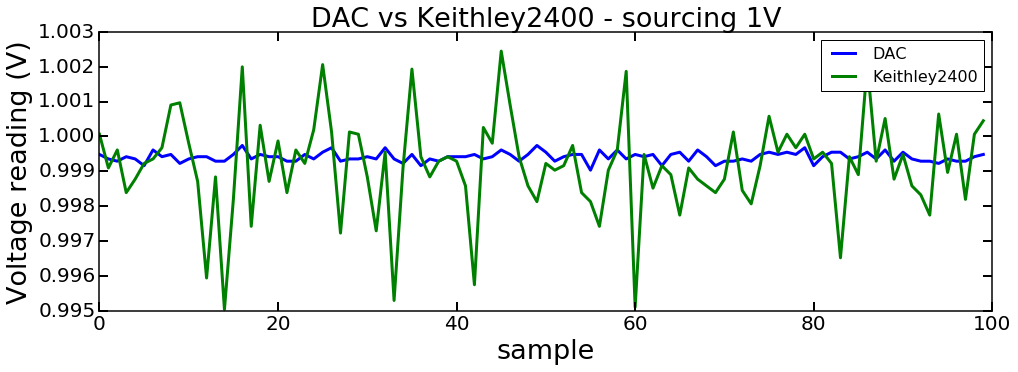
\includegraphics[width=0.75\linewidth]{images/experimentaltechniques/DACvKeithley.png}\\
            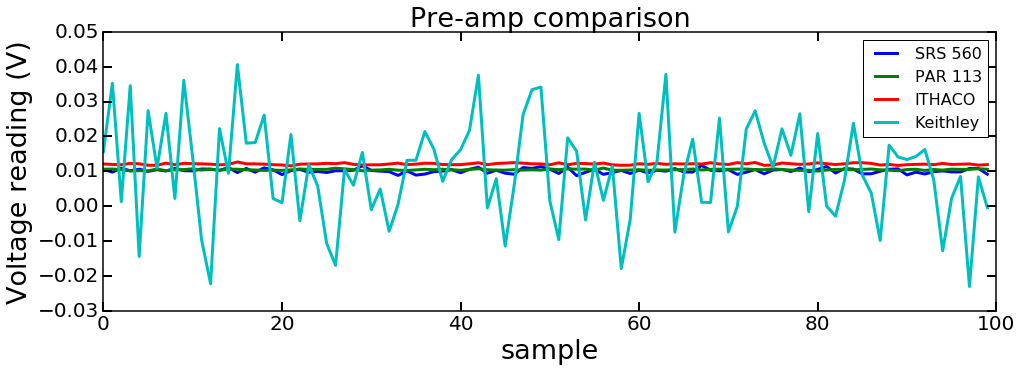
\includegraphics[width=0.75\linewidth]{images/experimentaltechniques/preams_k.png}\\
            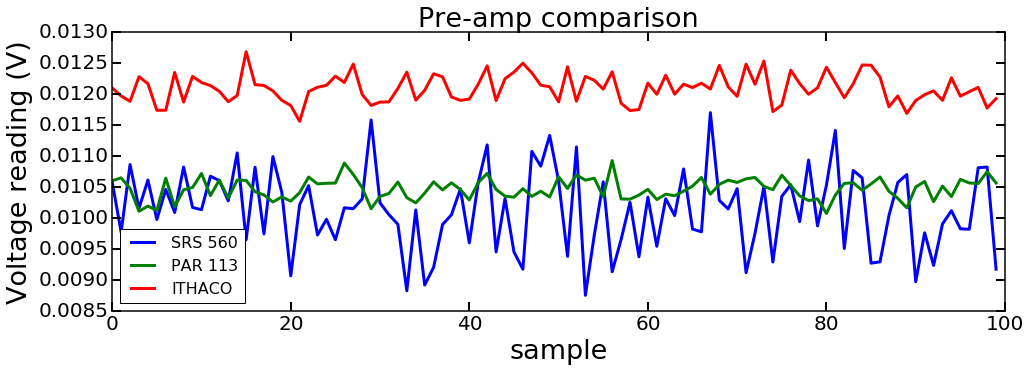
\includegraphics[width=0.75\linewidth]{images/experimentaltechniques/preamps.png}
            \caption[Noise characteristics of electronic measurement instruments]{
                Top: The voltage output of a Keithley 2400 SMU and a National Instruments BNC2110 Digital to Analog Converter
                measured over 10 seconds. Both were set to source 1 V.
                Middle: The output of a Keithley 2400 SMU before and after being passed through three different
                voltage pre-amplifiers.
                Bottom: The same data as above with only the amplified signals shown.
                }
            \label{fig:electronics_noise}
        \end{figure}
            
            \subsubsection*{Keithley 2400 SMU} 
            
            The Keithley 2400 is a source-measure unit (SMU) capable of 
            sourcing both current and voltage, and simultaneously measuring either current, voltage,
            or resistance. Its primary advantage is its wide operational range: it can source and measure
            up to 1 A in current mode, or 200 V in voltage mode.
            The Keithley 2400's wide operational range comes at the expense of precision; Figure \ref{fig:electronics_noise}A
            shows the measured output of a Keithley 2400 set to source 1 V, along with a similarly
            configured BNC2110 DAQ. The Keithley's output fluctuates by up to 0.5\% of the specified output value.
            The Keithley's precision can be improved by setting the `Range' parameter of the input and
            output: using the smallest range which still encompasses all the required values will provide the
            best precision.
            
            In practice, the Keithley 2400 is most useful for preliminary sample characterization (i.e. determining
            if a device conducts, and if so approximately what its resistance is) and for applying gate voltages.
            In the first case, the Keithley is useful because it can be manually configured by using the buttons
            on its face; for simple `Does the device conduct or not?'-type measurements this is often the most 
            convenient option.
            The Keithley 2400 is also particularly well suited to the latter use case: effectively gating graphene
            samples often requires gate voltages in the tens of volts, and the precise value of the supplied voltage
            is typically less critical for gating than for other applications.
            
            
            \subsubsection*{National Instruments Multifunction Data Acquisition Device (DAQ)} 
            
            The National Instruments Multifunction Data Acquisition Device (DAQ) is a source-measure unit 
            mounted on a PCI card. The PCI card must be physically installed in a computer, at which point
            it can be connected to an external connector block (e.g. the NI BNC-2110) which provides
            BNC connectors. Measurements using the DAQ must use instrument control programs installed
            on the computer which makes it less suitable for quick, one-of measurements.
            
            The DAQ makes the opposite trade-offs as the Keithley: 
            it provides high precision sourcing and measurement in a limited operational range.
            The DAQ can source and measure voltages from -10 V to 10 V.
            However, within this limited range the DAQ is more precise than the Keithley as seen
            in Figure \ref{fig:electronics_noise}A.
            The DAQ is particularly useful for applications which require high precision, for example
            providing the bias voltage in an I-V sweep or in a $V_\text{gate}$ vs $V_\text{bias}$ Coulomb
            blockade-type scan.
            
            \subsubsection*{Stanford Research System SR830} 
            
            The SR830 is a lock-in amplifier. Lock-in amplifiers operate by applying an AC drive to
            a device, measuring the resulting signal, and then multiplying the original drive
            and resulting signal and integrating over time.
            Because sinusoidal functions at different frequencies are orthogonal, the multiplication
            of the original drive and resulting signal and the subsequent integration combine to filter out
            components of the measured signal which are not at the same frequency as the original drive.
            Since most noise components will not be at the same frequency as the drive this technique
            is particularly effective at extracting a desired signal from a noisy measurement.
            
            In practice the SR830 is the preferred instrument for measuring resistance,
            provided the particular measurement is amenable to an AC bias.
            Additionally, the SR830 can only provide a voltage output; for applications which require a current bias 
            the output of the SR830 must be passed through a large resistor to convert the 
            voltage to a current. `Large' in this case means `large enough that the resistance of the device 
            being measured in
            series does not appreciably change the total resistance of the circuit'.
            
            \subsubsection*{Voltage and current preamplifiers}
            
            Voltage and current preamplifiers are useful for amplifying and filtering signals. Current
            preamplifiers are also useful for converting current signals into voltage signals.
            Figure \ref{fig:electronics_noise}B demonstrates the filtering capabilities of 
            a voltage preamplifier: it shows the output of a Keithley 2400 before and after
            being passed through several different preamplifiers (the raw Keithley signal has been
            rescaled to allow for direct comparison). All three preamplifiers drastically improve
            the cleanliness of the signal. Figure \ref{fig:electronics_noise}C compares the performance
            of the three preamplifiers; The PAR 113 provedes the best performance, while the 
            SRS 560 and ITHACO provide good accuracy at the expense of precision, and vice versa.
            
            %\subsubsection*{The probe station}
            
            
       
        
        \subsection{Transport measurements}
        
        This thesis is concerned with graphene's electronic properties, and these properties are most 
        readily observed via electrical transport measurements. There are a variety of factors which 
        affect what information can be gained via transport measurements,
        from the arrangement of the electrical contacts on the device to the dependent variables which 
        are varied in the course of the measurement. In this section I detail these factors, and describe
        their effects.
        
        \subsubsection*{Electronic contact configuration}
             
       
            Graphene devices can be measured using a variety of contact geometries, the simplest of which
            is the two-point configuration shown in Figure \ref{fig:contact_config}a. In this configuration
            the device being measured is contacted once at either end, and then these two leads are used both
            to bias the device and measure the result. This configuration has the advantage of being simple
            to fabricate and measure, however this simplicity comes at the cost of accuracy. Contacts between
            an electrical lead and a graphene device will necessarily create a contact resistance; when a 
            measurement is performed using the same leads which are used to bias the graphene the resulting
            signal is in fact a measurement of the device and the contact resistances in series. This situation
            is illustrated schematically in Figure \ref{fig:contact_config}b.
            
            To remove the confounding effect of contact resistances between the electrical leads and the graphene
            device one can perform measurements using a four-point configuration, illustrated in
            Figure \ref{fig:contact_config}c. This configuration employs two separate sets of leads, one set to
            bias the sample and a second set, placed in between the first set, to record the measurement. 
            In this case no current flows through the measurement leads, and thus there is no voltage drop
            across their contact resistances and the resulting measurement reflects only the properties of 
            the graphene device. This is illustrated schematically in Figure \ref{fig:contact_config}d.
            
            The contact configurations above are appropriate for measuring the longitudinal resistance, however it 
            is also useful to measure the lateral (or Hall) resistance. This requires a third contact configuration
            which is commonly called a Hall bar and which is illustrated in Figure \ref{fig:contact_config}e.
            In this configuration a bias current is applied through the two leads at the end of the device
            and the voltage is measured between either the horizontal or the vertical set of leads; the former 
            is equivalent to a four-point measurement of the longitudinal resistance while the latter measures
            the lateral (Hall) resistance.
            
         \begin{figure}
            \centering
            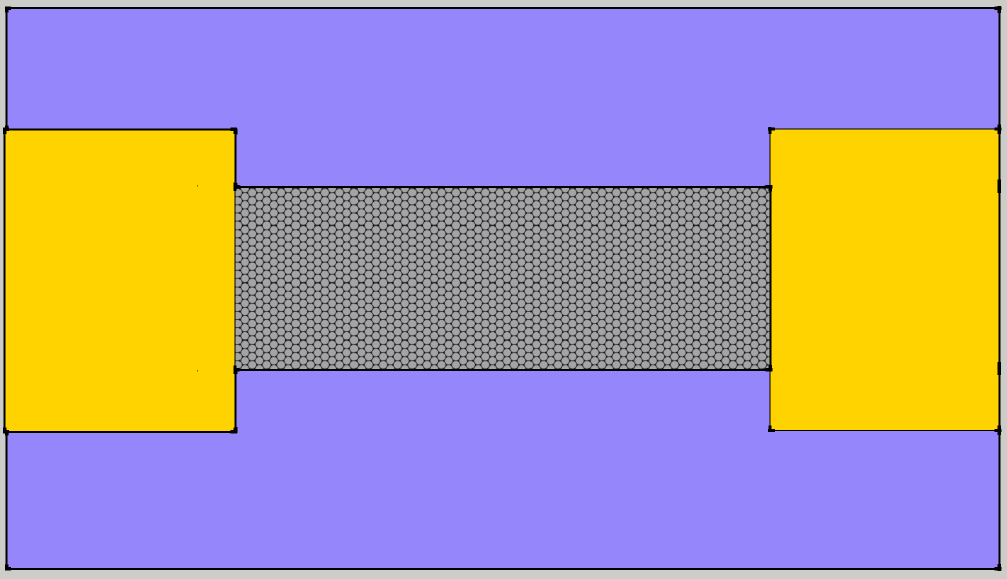
\includegraphics[width=0.4\linewidth]{images/experimentaltechniques/2pt-crop.png}
            \hspace{0.1\linewidth}
            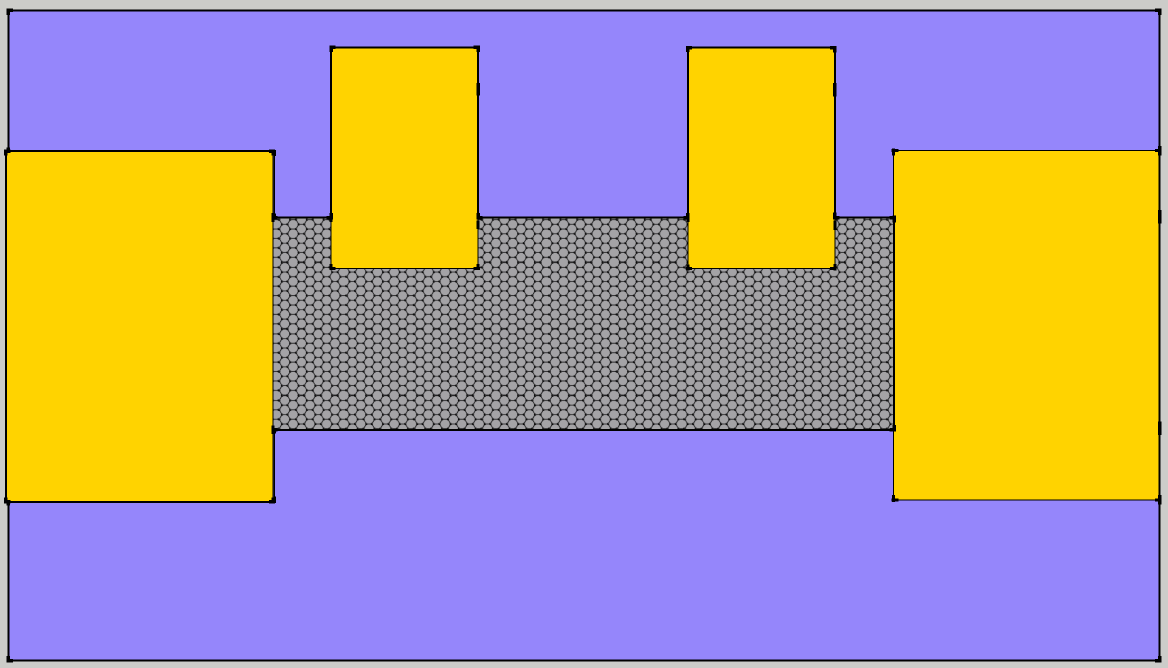
\includegraphics[width=0.4\linewidth]{images/experimentaltechniques/4pt-crop.png}\\
            \vspace{0.04\linewidth}
            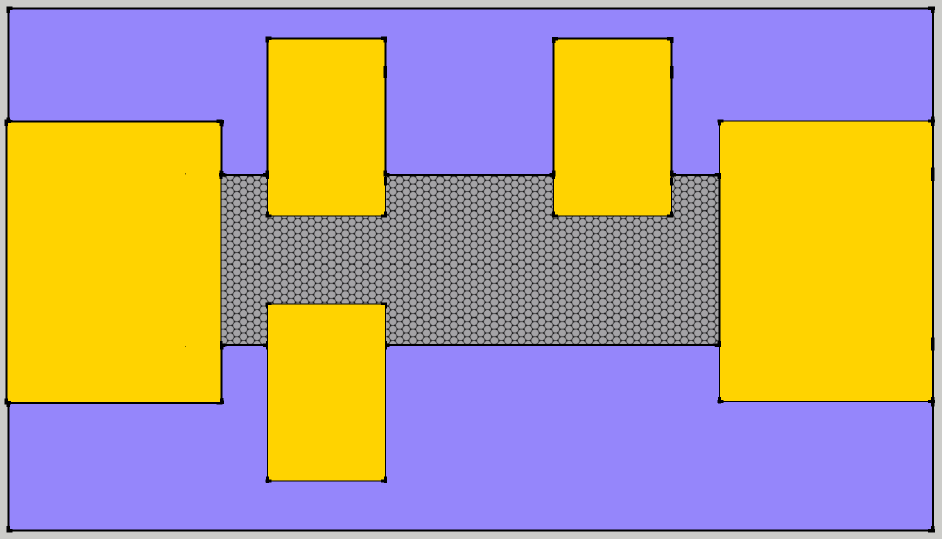
\includegraphics[width=0.4\linewidth]{images/experimentaltechniques/hallbar-crop.png}
            \hspace{0.1\linewidth}
            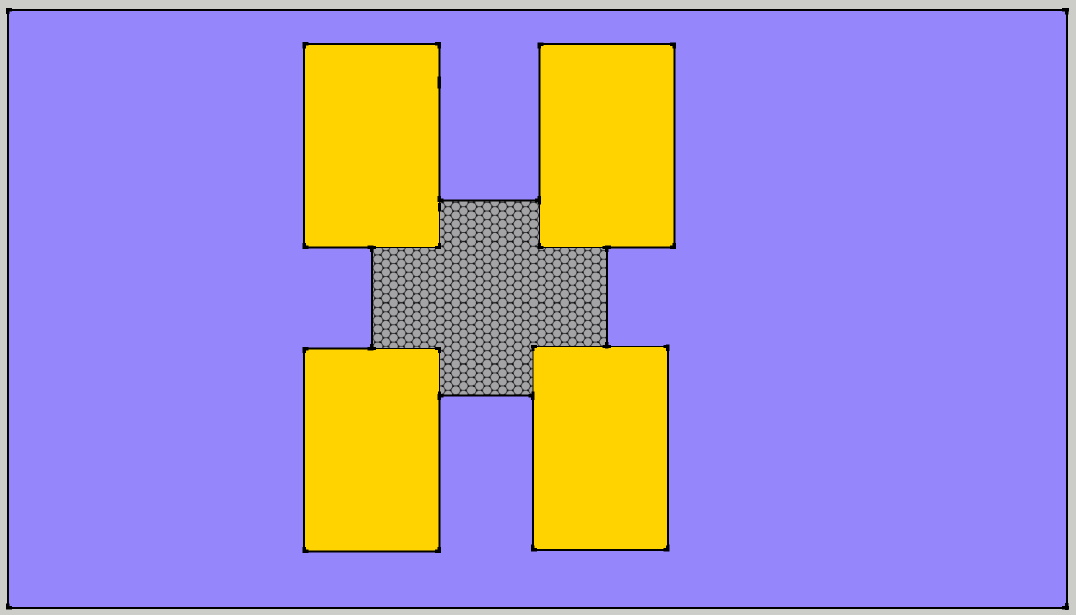
\includegraphics[width=0.4\linewidth]{images/experimentaltechniques/vdp-crop.png}\\
            \caption[Electronic contact configurations]{
                Schematic illustration of different electrical contact geometries. Clockwise from top-left
                they are two-point, four-point, van der Pauw, and Hall bar configurations. In each figure
                the purple region is the bare substrate, the grey region is graphene, and the yellow
                regions are the electrical contacts.
                }
            \label{fig:contact_config}
        \end{figure}
            
            Finally, it is sometimes useful to measure the sheet resistance of a device in addition to 
            its longitudinal and Hall resistances.
            This measurement requires another contact configuration which is illustrated in Figure XXX
            and which is commonly called the van der Pauw configuration\cite{van1958method}.
            The sheet resistance cannot be measured directly in this configuration; it must be calculated
            using the results of two preliminary measurements. First, current is made to flow along one
            edge of the sample and the voltage drop is measured across the edge opposite to the current flow.
            The resulting current and voltage values can be used to calculate a resistance.
            The same measurement is then repeated using the two edges perpendicular to the original edges.
            The sheet resistance can then be calculated from the two resistance measurements by numerically
            solving the following equation:
            
            \begin{equation}
                e^{-\pi R_{\text{vertical}}/R_S}+e^{-\pi R_{\text{horizontal}}/R_S}=1
            \end{equation}
           
        \subsubsection*{Types of transport measurements}
        
            The contact configurations described above are capable of measuring the resistance of a graphene
            device, however a single resistance measurement by itself is much less informative than
            a sequence of measurements taken as a function of some independent variable. For the graphene
            devices measured in the course of this research there are three particularly relevant
            independent variables: the bias voltage, gate voltage, and magnetic field.
            Here I describe the different types of transport measurements which can be performed by 
            varying each of these variables independently or together, and what information each
            type of measurement provides.
            
            \textbf{Gate sweeps}
            
            Measuring the resistance of a graphene sample as a function of the applied gate voltage 
            provides a basic characterization of the doping present in the graphene. For the
            devices described in this thesis the bottom surface of the chip on which the devices
            are fabricated serves as the gate.
            When a voltage is applied between the gate and the device the two form a capacitor, and
            the gate voltage serves to shift the Fermi level up or down, depending on the sign of the applied voltage. 
            By sweeping the gate voltage one can therefore sweep
            the Fermi level through the charge neutrality point (the point where graphene's conduction and valence bands touch). 
            The point where the Fermi level crosses the charge neutrality point will appear as a maximum
            in the measured resistance, so by measuring resistance as a function of gate voltage one
            can determine the polarity and degree of doping in a graphene device. This point is often called
            the Dirac point. Gate sweeps can also be used to confirm the presence of regions with different
            doping levels in graphene (e.g. pn junctions): gate sweeps on such devices will show two distinct
            resistance maxima corresponding to the two offset charge neutrality points in the regions with
            different doping levels.
             
            \begin{figure}
                \centering
                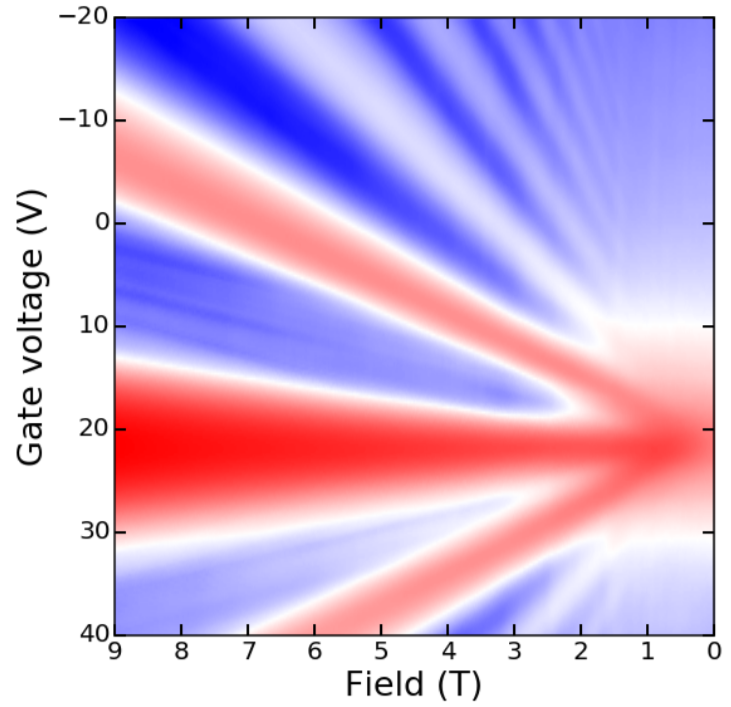
\includegraphics[width=0.4\linewidth]{images/experimentaltechniques/landau_levels.png}\\
                \caption[Landau levels in graphene]{
                    Resistance measurements of a graphene device as a function of gate voltage and
                    magnetic field. An initial peak in resistance at the Dirac point evolves into
                    Landau levels with increasing field.
                    }
                \label{fig:landau_levels}
            \end{figure}
            
            \textbf{Magnetic field sweeps}
            
            Measurements of graphene's resistance as a function of an applied magnetic field offer
            additional information about the graphene's characteristics. In particular, such measurements
            can be used to determine the carrier density and mobility.
            The carrier density can be determined in multiple ways. First, one can measure the
            longitudinal resistance as a function of an applied, perpendicular field. At low fields
            the resistance will display Shubnikov-de Haas oscillations. As described in Chapter 2, the 
            maxima of the oscillations are characterized by the equation $B_i = n \cdot h / 2 \cdot e \cdot i$
            where $i$ denotes the index of the oscillation and $n$ the carrier density. 
            By plotting the inverse of the field maxima against their indices one can therefore extract the carrier density:
            \begin{equation}
                \Delta\left(\frac{1}{B}\right) = \frac{1}{B_{i+1}}-\frac{1}{B_i} = \frac{2 \cdot e}{n\cdot h}\,.
            \end{equation}
            This technique is useful for situations where the device is not in a Hall bar configuration. For
            devices which are configured as Hall bars the Hall voltage can also be used to determine the carrier
            density, as well as the carrier mobility.
            
            As detailed in Chapter 2, the Hall resistance is given by $\rho_\text{xy} = B / e \cdot n$.
            The carrier density can therefore be extracted from the measured Hall voltage via 
            \note{why do we have to take the derivative here? instead of just dividing}
            \begin{equation}
                n = \left(e \, \frac{d\rho_\text{xy}}{dB}\right)^{-1} = \left(\frac{e}{I} \, \frac{dV_\text{xy}}{dB}\right)^{-1} \,.
            \end{equation}
            Armed with the carrier density and a measurement of the longitudinal resistance $\rho_\text{xx}$,
            we can also compute the carrier mobility via
            \begin{equation}
                \mu = \frac{1}{\rho_\text{xx} \cdot e \cdot n}
            \end{equation}
            
            Combining magnetic field and gate voltage sweeps into a single measurement offers a more complete picture
            of the behavior of a graphene device, as shown in Figure \ref{fig:landau_levels}. 
            In the figure we observe an initial resistance peak at the Dirac point, which evolves into several
            peaks corresponding to the formation of Landau levels as the applied magnetic field is increased.
            Examining the evolution and symmetry of oscillations in device measurements with increasing
            gate voltage or increasing magnetic field is a useful way to explore the physical origins of the oscillations.
            Often a single gate sweep or field sweep measurement can be rendered much more comprehensible by
            placing it in the context of a two dimensional plot like the one shown in Figure \ref{fig:landau_levels}.
            
           
            \textbf{Coulomb blockade measurements}
            
            Measurements of graphene's resistance as a function of both bias and gate voltage can be used to
            characterize confinement in the graphene. This is most useful in samples where the geometry
            of the graphene provide the confinement; recall from Chapter 2 that because electrons in graphene
            display Klein tunneling they cannot be confined by purely electrostatic means.
            For devices which provide spatial confinement, e.g. quantum dot-type devices, measurements
            of the differential conductance ($dI/dV$) will display a Coulomb blockade diamond pattern
            like the one shown in Figure \ref{fig:cb_diamond}. Information about the 
            Regular oscillations (like those shown in Figure \ref{fig:cb_diamond}) indicate that the device
            is operating as a single electron transistor
            and therefore that the relevant energy scale is the charging energy of adding another electron the the quantum dot.
            For devices with spatially smaller confinement the oscillations will become irregular, indicating 
            that the quantum mechanical energy associated with populating an additional state in a potential well
            is also relevant. This latter case is a consequence of the dispersion relation in graphene: the spacing
            between energy levels for massless carriers in a quantum box is much larger than for standard, massive carriers.
            
            \begin{figure}
                \centering
                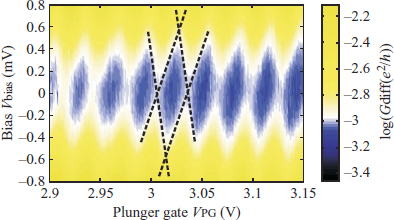
\includegraphics[width=0.5\linewidth]{images/experimentaltechniques/cb_diamond.jpg}\\
                \caption[Coulomb blockade diamonds in graphene]{
                    Differential conductance measurements as a function of gate and bias voltage in a 
                    graphene quantum dot device. The data display clear Coulomb blockade diamonds.
                    Adapted from \cite{guttinger2008coulomb}.
                    }
                \label{fig:cb_diamond}
            \end{figure}
            
            
    
\chapter{Results and Discussion}

\section{Graphene on flexible substrates}

    In this section I present the results of research which examines
    the mechanical properties of graphene devices stretched on flexible
    elastomer substrates. Using atomic force microscopy, electrical transport
    measurements, and mechanics simulations, we show that micro-rips form in the
    graphene during the initial application of tensile strain; however subsequent
    applications of the same tensile strain elastically open and close the existing
    rips. Correspondingly, while the initial tensile strain degrades the devices'
    transport properties, subsequent strain-relaxation cycles affect transport only
    moderately, and in a largely reversible fashion, yielding robust electrical
    transport even after partial mechanical failure. Graphene's combination of
    superlative electronic properties, extreme flexibility, and robust
    functionality after partial mechanical failure is unique among conducting thin
    films and lends itself to a variety of promising future device applications;
    the new understanding provided here of when and how graphene rips can directly
    impact the design of novel graphene-based devices which are required to
    function under strain.
    
    \subsection{Introduction}
    
        Recent advances in graphene production\cite{Kim2009, Bae2010, Lee2010} have
        enabled the fabrication of a variety of flexible, graphene-based electronic
        components, including transparent interconnects\cite{Kim2011}, high-performance
        capacitors\cite{El-Kady2012}, and transistors\cite{Lee2011}. The prospect of
        flexible and transparent graphene-based electronic devices suggested by these
        results raises an important question: are graphene's electrical properties and
        mechanical integrity robust under the strains graphene is likely to experience
        in such devices? Pristine graphene has an exceptionally high breaking
        strength\cite{Lee2008}, yet it may be susceptible to ripping, particularly if
        it has defects \cite{Kim2012} and/or strong  surface adhesion\cite{Sen2010}. It
        is still relatively unknown under what strain conditions substrate-supported
        graphene rips, and how the electrical properties are then altered.
        
        
        In this section I present the results of a research project in which 
        we combine atomic force microscopy (AFM), coarse-grained
        mechanical simulations, and electrical transport measurements to study the
        effects of lateral strain on rips in graphene. We find that graphene adhered to
        a flexible substrate and then stretched laterally can develop small rips with
        only 1\% applied strain. However, even with ripping, the electrical properties
        remain relatively robust: introducing small rips slightly increases the
        resistance, but subsequent strain-relaxation cycles over the same strain range
        change transport only modestly, and in a largely reversible fashion. Such
        resilience is atypical for conducting thin films, which typically demonstrate
        rapid and irreversible device failure after the onset of rip
        formation\cite{Cairns2000,Fortunato2002}.
    
        This new understanding of when and how graphene rips, and how its electrical
        properties are thereby altered is immediately applicable to the implementation
        and production of devices which include the graphene-based components mentioned
        above. Some applications, for instance frequency-tuned RC circuits using
        graphene capacitors and interconnects, would require careful consideration of
        what strains the device can withstand while keeping strain-induced variations
        in the electronic properties of graphene within the required specifications.
        Likewise, in applications such as portable consumer electronics where low power
        consumption is a priority the increased resistance of strained graphene films
        may limit the potentially applicable strain, or require the use of more
        complicated interconnect geometries\cite{Kim2011}. Graphene's exceptional
        resilience as described here may also motivate its inclusion in device
        applications where other conducting thin films have been used to date;
        bio-integrated devices\cite{Viventi2010} are especially appealing candidates
        because of the difficulty involved in replacing devices installed \textit{in
        vivo}, as well as because of graphene's non-toxicity.
       
    \subsection{Device configuration}
    
        \begin{figure}
        \centering
        \vspace{0.2cm}
        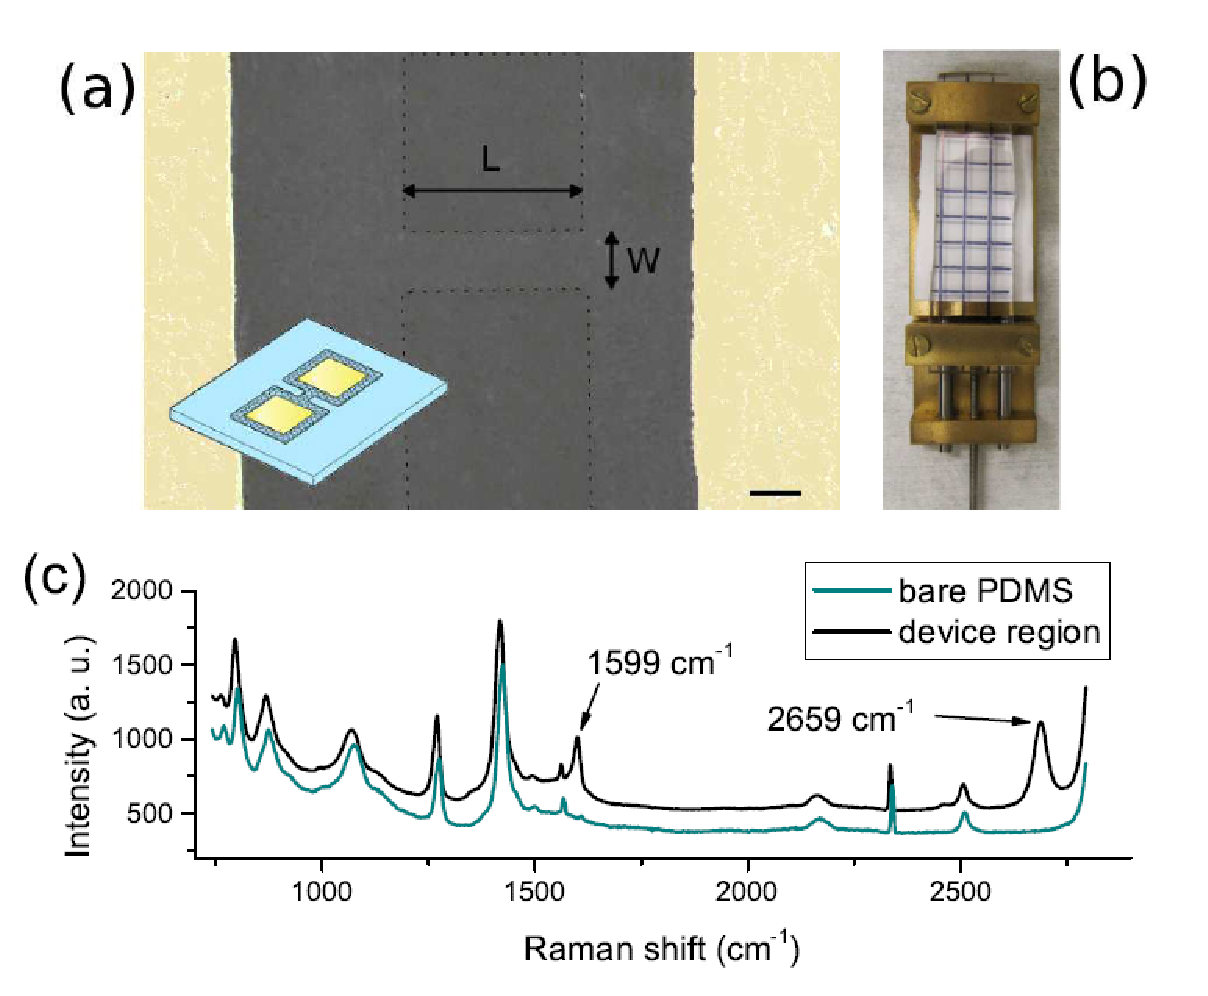
\includegraphics[width=0.75\linewidth]{images/resultsanddiscussion/rippingpaper/Figure1.eps}
        \caption[Device geometry and measurement apparatus for uniaxially strained graphene]
            {\textbf{(a)} False-color optical image of a graphene bridge device
            (outlined by dashed line) patterned on a PDMS substrate with gold contact pads
            (light yellow). The length (L) and width (W) of the bridge are described in the
            text. The scale bar is 25 $\mu$m. Inset: A schematic illustration of the device
            geometry. \textbf{(b)}  The mechanical stretching stage with PDMS inserted
            between the clamps. The devices are stretched along the axis of the
            micro-bridge. \textbf{(c)} Offset Raman spectra for a bare PDMS region and a
            graphene device region. The graphene G and 2D peaks, at 1599 cm$^{-1}$ and 2659
            cm$^{-1}$ respectively, in the spectra from the device region confirm the
            presence of graphene.}
        \label{fig:rip-device}
        \end{figure}
   
        Devices consisted of patterned graphene placed on flexible polydimethylsiloxane
        (PDMS) substrates. The devices were fabricated using a modified transfer
        printing process, similar to that described in Ref \cite{Kim2009}.
        Single-layer graphene was grown using established chemical vapor deposition
        (CVD) techniques \cite{Li2009}, and then transferred to a copper-coated silicon
        wafer where it was patterned using photolithography and reactive ion etching.
        Next, a piece of PDMS was mechanically pressed onto the silicon wafer, and the
        copper was then etched to leave patterned graphene on the PDMS
        substrate\cite{Lee2010}. Raman spectroscopy was used to confirm the presence of
        graphene on the PDMS as shown in Figure \ref{fig:rip-device}c; the shape of the Raman 2D
        peak\cite{Ferrari2006}, as well as subsequent AFM measurements verified the
        single-layer character of the graphene. Finally, shadow-mask evaporation was
        used to deposit Ti/Au contact pads. The device geometry is illustrated in
        Figure \ref{fig:rip-device}a: a narrow graphene bridge connects two large graphene pads, each of
        which is covered with a Ti/Au contact pad. We studied 13 different devices
        having bridge aspect ratios ranging from 1.5:1 to 12:1 (length:width) and
        widths of 100, 50, and 25 $\mu$m. The data in this manuscript focuses on a
        device with a bridge width of 25 $\mu$m and an aspect ratio of 2:1. The data
        for all samples yielded similar qualitative results. Quantitative differences
        in transport data between different devices were uncorrelated with the bridge
        dimensions, and instead seemed to be dominated by pre-existing rips in the
        graphene, which are often introduced during the graphene transfer
        process\cite{Kim2012}.

        AFM and transport measurements were performed while the PDMS substrate was
        mounted in a mechanical stretching stage, as shown in Figure \ref{fig:rip-device}. The substrate
        was clamped at either end, and then strained by turning the threaded rod, which
        laterally moves the sliding clamp along its guide rails. A mechanical stepper
        motor was used to control the stretching stage position to ensure
        reproducibility. Variable device positioning on the substrate as well as slight
        variations in substrate thickness preclude exact conversion between strain
        applied to the substrate and to the device, therefore `turns of the stretching
        stage control rod' were used as the controlled variable. Each turn strains the
        substrate by approximately one percent, and we estimate that the strain applied
        to the graphene differs from that applied to the PDMS substrate by no more than
        ten percent. However, our conclusions are unaffected by this uncertainty, as
        variations in the magnitude of applied strain between devices only shift the
        strain axis of the data while preserving the observed trends. Optical
        observations indicated that the Ti/Au pad adhesion to the substrate was robust
        and did not slip during measurements. Transport measurements were performed by
        placing micro-manipulator probes in contact with the gold contact pads at each
        strain value, and AFM measurements were performed with an Asylum Research
        MFP-3D.
        
    \subsection{Rip formation under strain}
 
        \begin{figure}
        \centering
        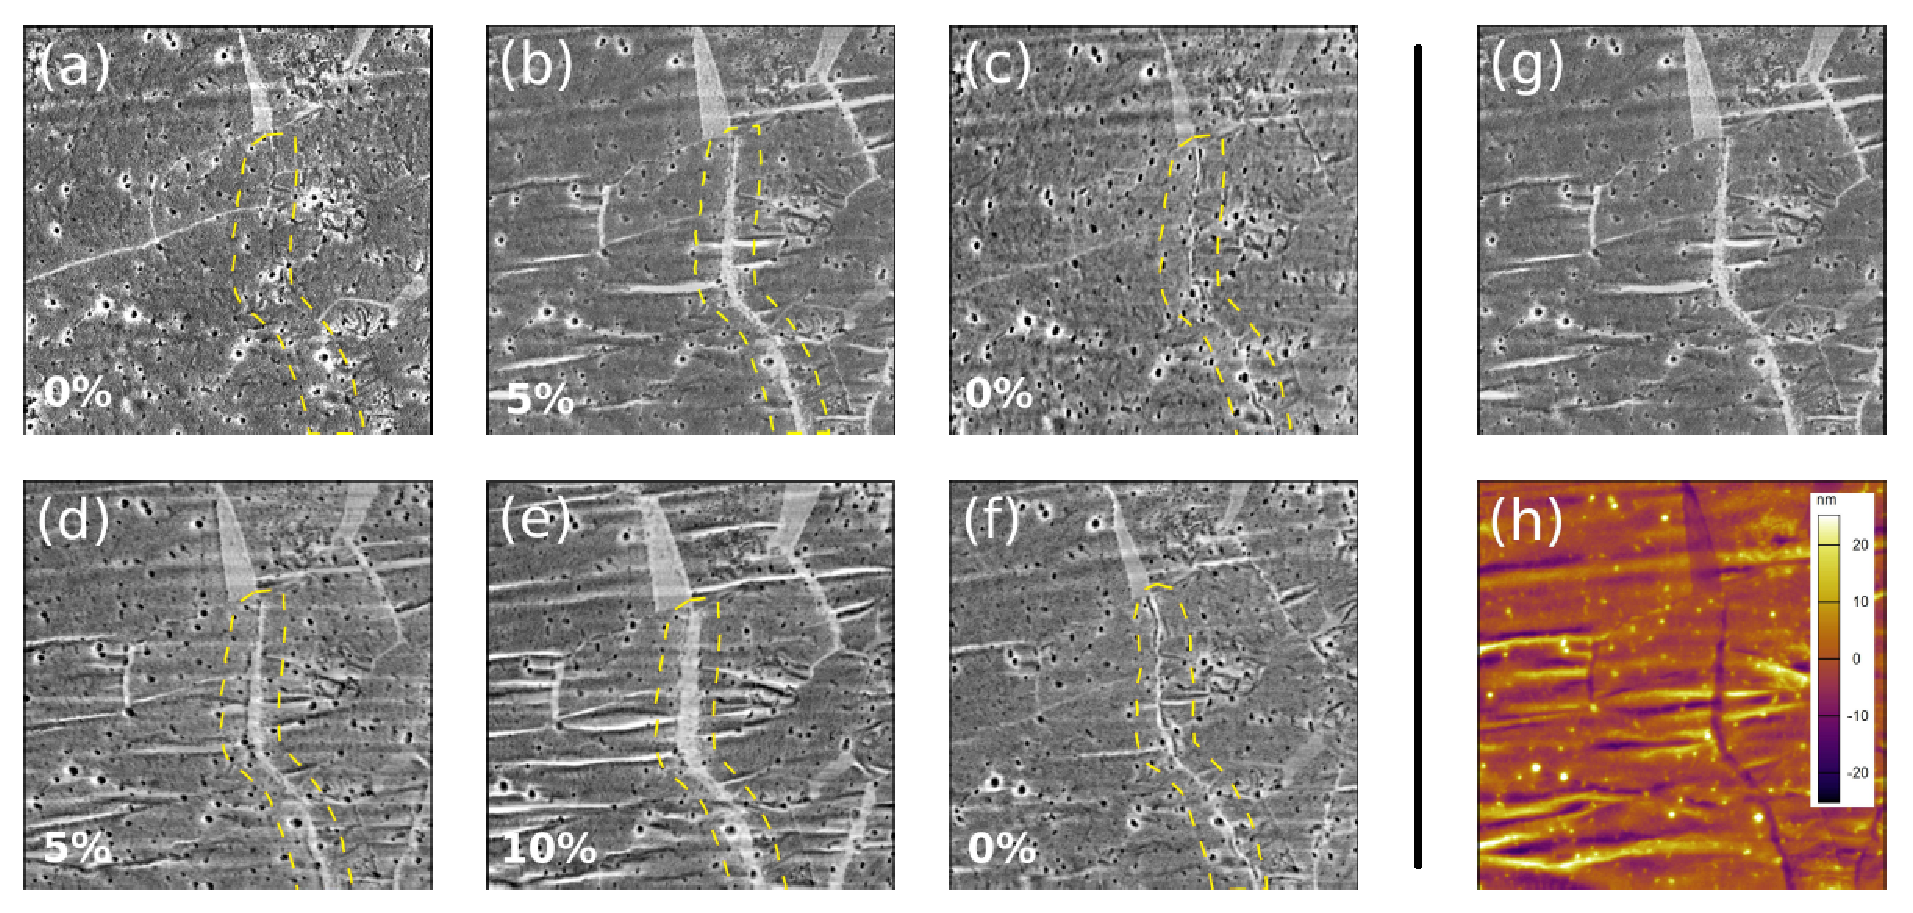
\includegraphics[width=\linewidth]{images/resultsanddiscussion/rippingpaper/Figure3.eps}
        \caption[AFM measurements of uniaxially strained graphene]
            {\textbf{(a-f)} AFM phase measurements of graphene on a polymer
            substrate at approximately 0, 5, 0, 5, 10, and 0 percent strain (applied along
            the horizontal axis), as labeled. Rips are evident as light-gray, elongated
            vertical features. An example of a rip that opens and closes with applied
            strain is indicated by the dashed line. Dark spots present in each image are
            debris on the substrate surface; white halos surrounding some of the debris are
            indicative of graphene slightly delaminating from the substrate. Elongated
            horizontal features are strain-dependent wrinkles. \textbf{(g)} AFM phase and
            \textbf{(h)} height data. Variations in the height data distinguish between
            wrinkles and rips in the graphene, which have similar signatures in the phase
            data. The scanned area in each image is 25 $\mu$m$^2$.}
        \label{fig:rip-afm}
        \end{figure}
   
        \subsubsection*{Experimental results}
        
        Figures \ref{fig:rip-afm}-f show AFM phase images of graphene in the bridge region of a device
        at 0, 5, 0, 5, 10, and 0 percent strain applied along the horizontal axis of
        the images. Both rips and delaminations caused by wrinkles appear as a function
        of strain, and can be distinguished via AFM height data: Figures \ref{fig:rip-afm}g and \ref{fig:rip-afm}h show
        that wrinkles have corresponding undulations in the height data (peaks and
        dips) while rips are indicated by a uniform depression (consistent with the
        substrate exposed between graphene regions). In Fig. 2, the vertical features
        are rips and the majority of the horizontal features are wrinkles.
        
        \ref{fig:rip-afm}
        
        The opening and closing of rips is clear in the Figure:  the unstrained device
        (Fig. \ref{fig:rip-afm}a) exhibits some small rips and defects. When the substrate is
        mechanically stretched (Fig. \ref{fig:rip-afm}b) the existing rips widen and new rips form;
        when the applied strain is relaxed (Fig. \ref{fig:rip-afm}c), pre-existing defects return to
        nearly their original condition and newly formed rips close. Subsequent
        strain-relaxation cycles over the same strain range re-open existing rips (Fig.\ref{fig:rip-afm}d), 
        but proceeding to a higher strain range forms new rips and widens
        pre-existing ones (Fig.\ref{fig:rip-afm}e), which then close less completely when the strain
        is relaxed (Fig.\ref{fig:rip-afm}f). The strain values at which we observe micro-rip formation
        are substantially lower than the reported fracture strength of
        graphene\cite{Lee2008}, however the tensile strength of graphene is strongly
        susceptible to defects such as holes and tears\cite{Lee2013}. Although graphene
        produced by CVD is known to be polydomain, it has been shown that rips in
        graphene do not preferentially follow grain boundaries\cite{Kim2012}. Rather,
        the fabrication procedures used to generate patterned graphene devices on
        polymer substrates routinely introduce rips and other defects in the graphene,
        which accounts for the mechanical failure observed at low strain values.
 
        \begin{figure}
        \centering
        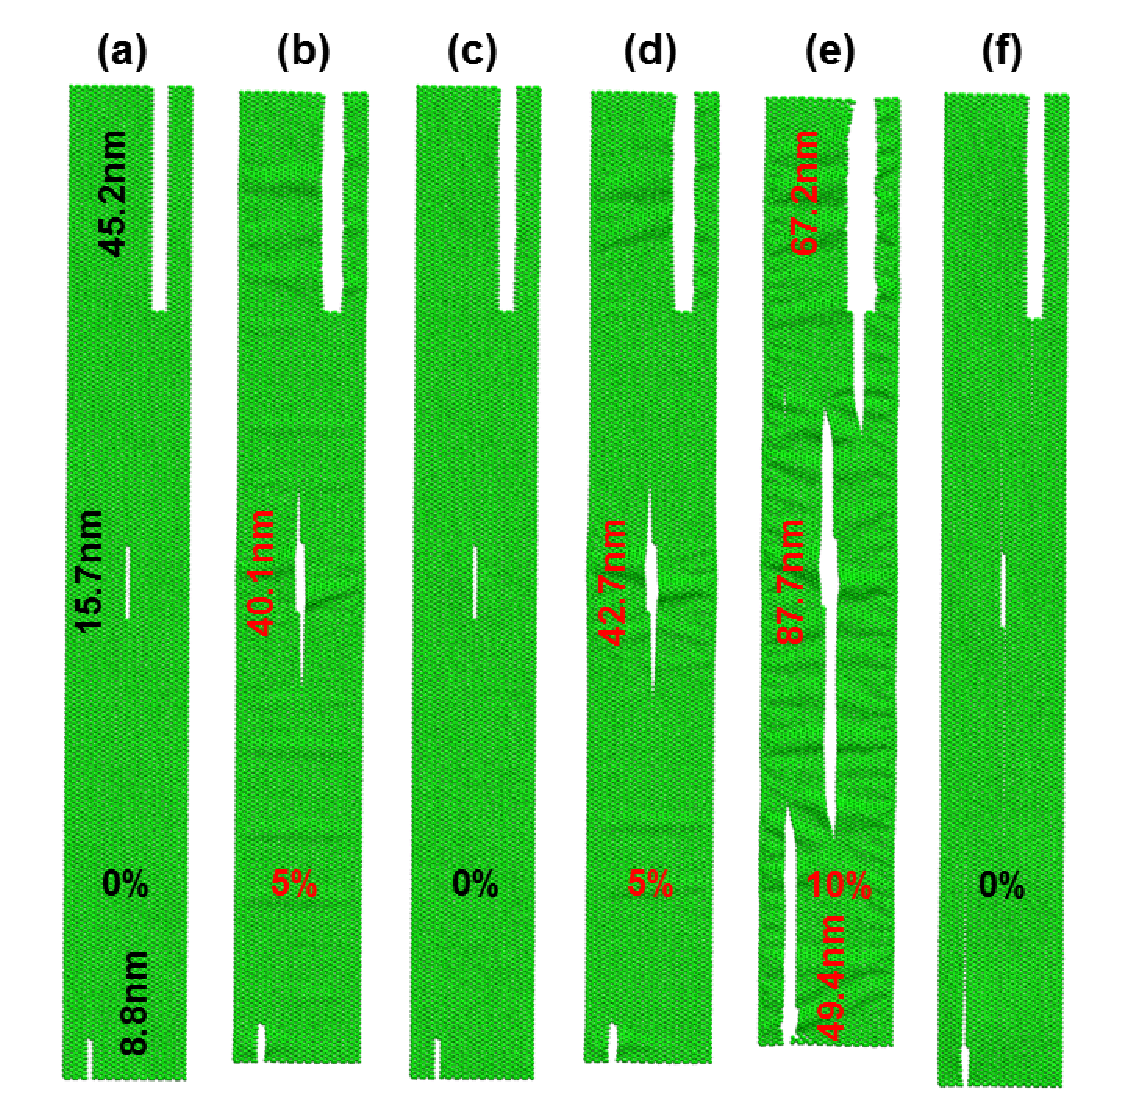
\includegraphics[width=0.5\linewidth]{images/resultsanddiscussion/rippingpaper/Figure4.eps}
        \caption[Simulations of rip formation in uniaxially strained graphene]
            {Coarse-grained simulations show the elastic opening and closing of
            rips during initial and subsequent tensile loading cycles, in good agreement
            with AFM measurements in Figure 2. The graphene region was simulated at 0, 5,
            0, 5, 10, and 0 percent strain applied along the horizontal axis, as labeled.
            Values given in nm refer to the rip lengths. The vertical contraction of the
            graphene region at higher strain values is due to the Poisson effect.}
        \label{fig:rip-simulation}
        \end{figure}
       
        \subsubsection*{Simulation results}
        
        To shed light on the underlying mechanism of the rip formation and evolution,
        our collaborators simulated rip formation and the subsequent elastic opening and closing of
        rips in graphene, via a coarse-grained (CG) modeling scheme\cite{Zhu2014}.
        The following description of simulation results describes their work.
        Given the prohibitive simulation expense to model rips of real size in
        experiments (microns in length), they simulated a scaled-down model of a graphene
        monolayer with a size of 24 nm by 200 nm (Fig. \ref{fig:rip-simulation}). Three pre-cracks of various
        sizes were introduced in the model (Fig. \ref{fig:rip-simulation}a) to mimic the pre-existing defects
        in the as-made sample. Each CG bead in the graphene interacts with a virtual
        substrate via a Lennard-Jones potential\cite{Scharfenberg2011} $V_{gs}(r)
        =4\varepsilon_{gs} \left( \frac{\sigma_{gs}^{12}}{r^{12}} -
        \frac{\sigma_{gs}^6}{r^6} \right)$, where $\varepsilon_{gs}=0.01844 \,
        \text{eV}$ and $\sigma_{gs}=0.29 \, \text{nm}$, which gives rise to an adhesion
        energy around 0.044 eV/nm$^{2}$. In addition, the CG beads on the four outer
        edges of the simulation model were not allowed to slide relative to the
        substrate so that the tensile loading of the graphene can be applied by
        stretching the substrate along the horizontal direction, similar to the
        experimental setup.
        
        As the applied tensile strain first increases to 5\%, the stress concentration
        near the tips of the short middle crack ($\sim$15.7 nm in length) becomes
        sufficiently high to cause the propagation of the short crack in both
        directions. Due to the nature of displacement loading, the driving force for
        crack propagation decreases as the crack extends. As a result, the middle crack
        stops advancing at a length of $\sim$40.1 nm (Fig. \ref{fig:rip-simulation}b). Upon unloading of the
        tensile strain the elongated middle crack closes, nearly fully recovering the
        original shape of the graphene (Fig. \ref{fig:rip-simulation}c); however, the atomic bond breaking in
        graphene during crack propagation is not reversible. Consequently, the graphene
        cannot fully recover its original mechanical integrity.
        
        Further tensile loading up to 5\% causes the cracks to reopen but further
        extension of the cracks is shown to be negligible (Fig. \ref{fig:rip-simulation}d), largely due to a
        lack of sufficient driving force for crack propagation. The application of a
        tensile loading of 10\% provides sufficient driving force to cause all three
        cracks to extend significantly. The crack propagation eventually saturates due
        to the decreasing driving force under displacement loading (Fig. \ref{fig:rip-simulation}e). Upon
        unloading to zero strain, all newly formed cracks close, resulting in a
        graphene morphology nearly identical to its original shape (Fig. \ref{fig:rip-simulation}f), similar
        to the experimental observation (Fig. \ref{fig:rip-afm}e to Fig. \ref{fig:rip-afm}f).
        
        Simulations also show the formation of delaminations and horizontal wrinkles in
        graphene upon tensile loading and the disappearance of such features upon
        unloading, which agrees with the experimental observations (Fig. \ref{fig:rip-afm}). We
        attribute the formation of these delamination and wrinkle features to the
        combined effect of a mismatch in Poisson's ratios between graphene and the PDMS
        substrate and the relatively weak graphene/PDMS interfacial bonding. In
        addition, recent studies show that the location of wrinkles in graphene can be
        guided by the debris distribution on the substrate surface \cite{Zhu2014b},
        consistent with our experimental observations in Fig. \ref{fig:rip-afm}.
        
        The close agreement between the experimental observations and mechanics
        simulations yields two conclusions: first, pre-existing defects play a decisive
        role in the formation of rips in graphene. The concentration of stress near the
        edge of rips causes graphene to mechanically fail at lower strain values than
        its high intrinsic breaking strength would suggest, therefore when fabricating
        flexible graphene-based devices optimizing the mechanical integrity of the
        graphene is important not only to maximize the initial quality of the device
        but also its subsequent durability. Second, the generic nature of the
        simulations suggests that the first conclusion is generally applicable to thin
        membrane devices; while other thin films may not have the flexibility,
        transparency, and electronic properties of graphene the simulations suggest
        that their failure modes when supported by flexible substrates are similar.

    \subsection{Resistance changes under uniaxial strain}
    
        \begin{figure*}
        \centering
        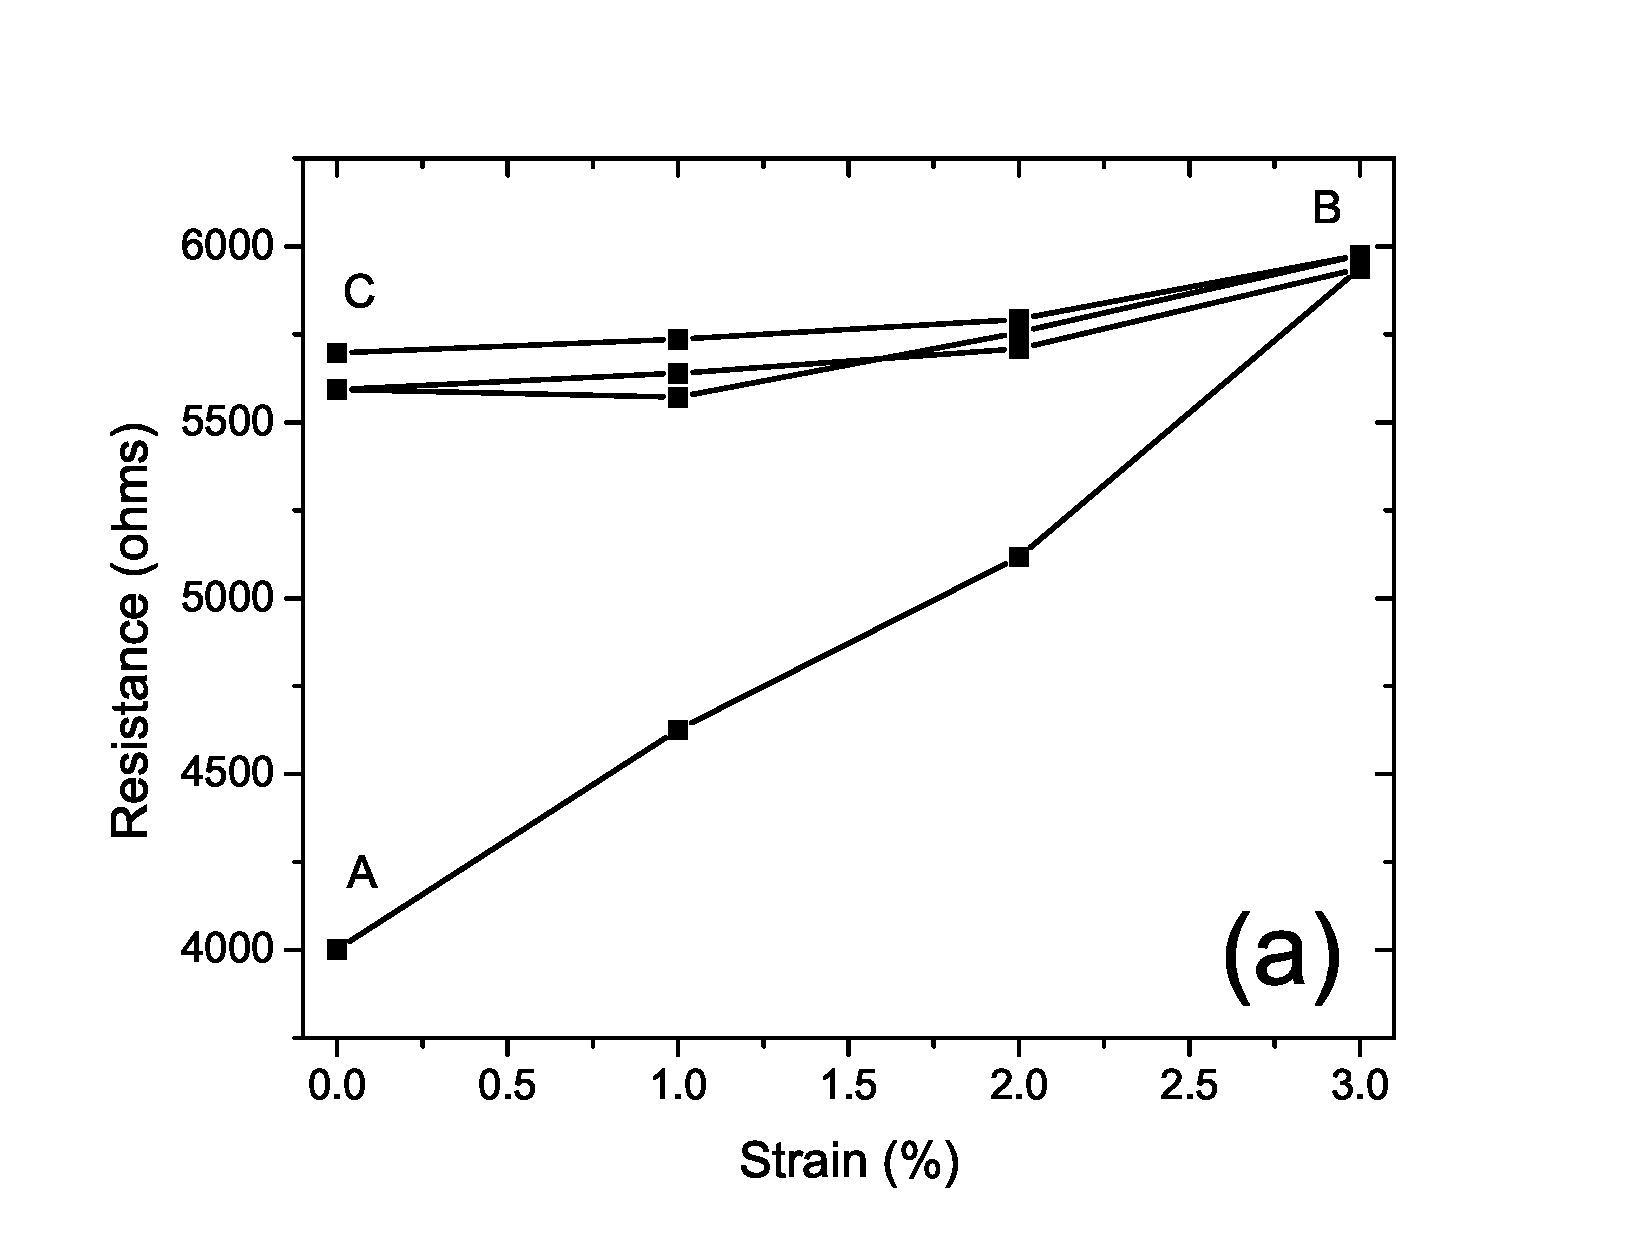
\includegraphics[width=0.49\linewidth]{images/resultsanddiscussion/rippingpaper/Fig2a.eps}
        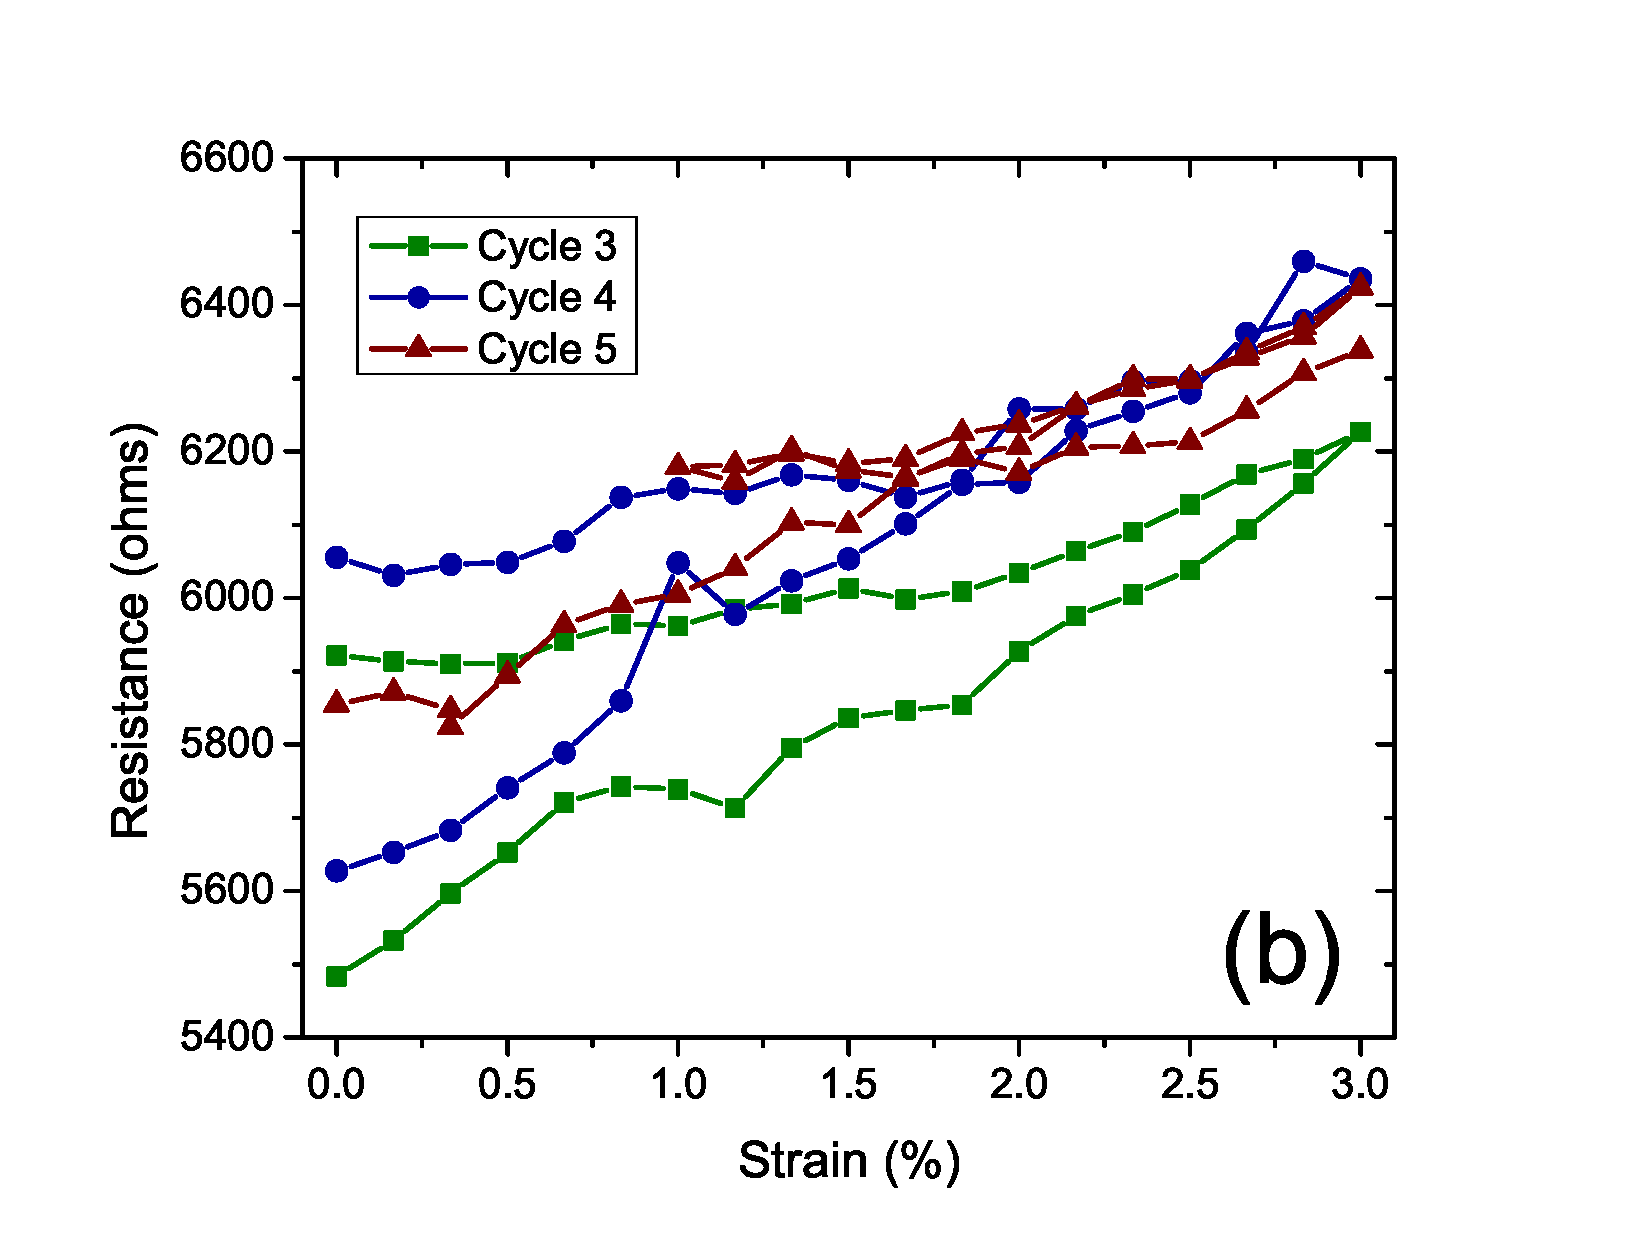
\includegraphics[width=0.49\linewidth]{images/resultsanddiscussion/rippingpaper/Fig2b.eps}
            \caption[Resistance vs strain for graphene on flexible substrates]{
                \textbf{(a)} Electrical resistance of a graphene device vs. applied tensile strain. 
                The initial application of strain significantly increases the resistance while subsequent 
                strain-relaxation cycles over the same strain range yield smaller, mostly reversible 
                changes in the resistance. \textbf{(b)} Three consecutive strain-relaxation cycles 
                (Cycles 3,4,5), showing largely reversible transport characteristics. Three arb. units 
                correspond roughly to three percent applied strain.}
        \label{fig:rip-RvsStrain}
        \end{figure*}
   
        The behavior of the rips determines the electrical transport as a function of
        strain, as evident in Figure \ref{fig:rip-RvsStrain}. Figure \ref{fig:rip-RvsStrain}a 
        demonstrates three important features
        of the data: first, during the initial application of strain (A to B in the
        Figure) the resistance increases (for this sample, by approximately 43
        percent). Typical values for this initial increase in other devices ranged from
        20 to 40 percent of the starting resistance. Second, the resistance of the
        device decreases as the applied strain is relaxed (from B to C) by 7 percent
        for this device, and typically by between 6 and 14 percent. Finally, in
        subsequent strain-relaxation cycles over the same strain range the resistance
        changes only moderately, and in a largely reversible fashion.
        
        The transport behavior can be explained by the opening and closing of rips: in
        the unstrained device, small rips largely determine the initial resistivity.
        The device's resistance increases when the substrate is mechanically stretched,
        due to the widening of existing rips and formation of new ones; subsequent
        strain-relaxation cycles over the same strain range, which re-open and close
        existing rips, generate largely reversible changes in resistance. This
        reversibility is demonstrated in Figure \ref{fig:rip-RvsStrain}b; data from the same device recorded
        during the third, fourth, and fifth strain-relaxation cycles are shown in
        green, blue, and red respectively. In each case the resistance changes by
        $\sim$14\% for $\sim$3\% applied strain, and returns to within 8\% of its
        original value. Proceeding to a higher strain range forms new rips, consistent
        with a jump in resistance when the strain range is increased. This behavior --
        an increase in resistance with the initial application of tensile strain,
        followed by moderate and reversible changes in the resistance during subsequent
        strain-relaxation cycles over the same strain region -- persists up to
        approximately 15\% applied strain, at which point the devices become
        permanently non-conducting.
        
        Previous experimental work has demonstrated reversible transport changes in
        strained graphene, either by depositing graphene on pre-strained substrates so
        as to create controlled crumpling\cite{Zang2013} and buckling\cite{Wang2011},
        by patterning complex interconnect geometries\cite{Kim2011,Lee2010}, or by
        measuring transport across macroscopic graphene films\cite{Kim2009,Bae2010}. In
        comparison, this work demonstrates the continuing robustness of device
        functionality \textit{after} partial mechanical failure. Such resilience is
        distinctly atypical for conducting thin films: similar studies performed on
        tin-doped indium oxide (ITO)\cite{Cairns2000} and zinc
        oxide\cite{Fortunato2002} reported rapid and irreversible device failure after
        the onset of rip formation.  One potential explanation for graphene's
        exceptional resilience is its morphological simplicity: as a two-dimensional
        membrane re-establishing electrical contact between two sides of a rip is as
        simple as overlaying two sheets of paper, while for typical three-dimensional
        thin films the process is more similar to fitting two halves of a snapped
        pencil back together.
        

    \subsection{Summary}

        In summary, we have observed the formation and subsequent evolution of
        micro-rips in graphene using atomic force microscopy. While an initial
        application of tensile strain introduces new mechanical defects, successive
        strain-relaxation cycles over the same strain range elastically open and close
        the existing rips. Mechanics simulations further reveal the underlying
        deformation and failure mechanisms of the graphene sample under initial and
        subsequent cyclic tensile loadings, which agree well with the AFM measurements.
        This mechanical effect has a corresponding electrical effect: the graphene's
        transport properties are degraded by the initial application of strain, but
        show small, mostly reversible changes during ensuing strain-relaxation cycles.
        
        Graphene's combination of superlative electronic properties, extreme
        flexibility, and robust functionality after partial mechanical failure is
        unique among conducting thin films and lends itself to a variety of promising
        future device applications. For applications with stringent component
        requirements such as RC frequency filters or devices used for precise metrology
        the onset of rip formation and the subsequent variation in electrical
        properties described here are crucial design considerations. Similarly, the
        interplay between strain-dependent resistance increases and power consumption
        requirements may impose design limits on the use of graphene in next-generation
        flexible displays and touchscreens. If graphene is to be used in applied
        devices outside the laboratory a thorough understanding of when and how it will
        fail is essential. In this manuscript we present a detailed description of
        precisely this situation, with exciting implications for robust, graphene-based
        electronic devices.

        We thank Scott Maclaren (UIUC MRL/CMM) for technical assistance on this project. This work was
        supported by NSF grants \#1069076 and \#1129826, NSF-CMMI grant
        \#1130364 and NSF-NEB grant \#486171, and was carried out
        in part in the Frederick Seitz Materials Research Laboratory Central
        Facilities, University of Illinois.



\section{Graphene on ferroelectric substrates}


    In this section I report the results of a project where my collaborators and I performed electrical transport measurements on graphene p-n junctions formed via simple modifications to a PbZr$_{0.2}$Ti$_{0.8}$O$_3$ substrate, combined with a self-assembled layer of ambient environmental dopants. We show that the substrate configuration controls the local doping region, and that the p-n junction behavior can be controlled with a single gate. Finally, we show that the ferroelectric substrate induces a hysteresis in the environmental doping which can be utilized to activate and deactivate the doping, yielding an `on-demand' p-n junction in graphene controlled by a single, universal backgate.

    \subsection{Introduction}
    
        Graphene is a subject of intense research interest due to the enormous potential of its electronic and mechanical properties\cite{Geim2007}. In particular, p-n junctions in graphene have great potential for both fundamental research and commercial applications, and have been utilized to study the quantum Hall effect \cite{Williams2007, Ozyilmaz2007, Velasco2010} and Klein tunneling\cite{Stander2009, Young2009} as well as to fabricate flexible transistors\cite{Kim2010}. Previous work on p-n junctions in graphene employed multiple electrostatic gates \cite{Meric2008, Williams2007, Ozyilmaz2007, Huard2007, Liu2008, Stander2009, Velasco2009, Velasco2010, Young2009}, charge transfer from the controlled deposition of chemical adsorbates \cite{Farmer2009,Lohmann2009,Brenner2010,Cheng2011,Sojoudi2012,Seo2014,Park2015}, high current-induced charging of trap states in the substrate \cite{Chiu2010}, or periodically poled ferroelectric substrates\cite{Baeumer2015}.

        In this section we report the fabrication of p-n junctions in graphene deposited on a uniformly poled ferroelectric substrate. The local doping in our devices is accomplished by combining simple modifications to a lead zirconium titanate (PbZr$_{0.2}$Ti$_{0.8}$O$_3$) substrate -- the evaporation of thin SiO$_2$ films in some regions -- with a self-assembled layer of environmental dopants. We find that the PbZr$_{0.2}$Ti$_{0.8}$O$_3$ substrate modulates the doping effect of the adsorbed dopants: devices are exposed to ambient conditions after fabrication whereupon experimental observations confirm both the presence of adsorbed dopants (likely primarily H$_2$O) and their enhanced doping effect on the PbZr$_{0.2}$Ti$_{0.8}$O$_3$ relative to the SiO$_2$.
        Furthermore, we demonstrate that the PbZr$_{0.2}$Ti$_{0.8}$O$_3$ substrate induces a hysteresis in the environmental doping which can be used to activate and deactivate the doping via the application of large gate voltages. We employ this effect to create p-n junctions which can be reversibly transitioned between p-n junction and uniformly conducting configurations.

    \subsection{Device configuration}
    
        Devices consist of graphene micro-ribbons deposited on substrates which are partially covered by a thin layer of evaporated SiO$_2$, and contacted in a four-point geometry, as illustrated in Figures \ref{fig:devices}a-c. An SEM micrograph of a typical device is shown in the inset of Figure \ref{fig:devices}d. The devices are fabricated using standard lithography and deposition techniques on thin-film ferroelectric substrates. For the ferroelectric substrates, 120 nm thick (001)-oriented lead zirconium titanate (PbZr$_{0.2}$Ti$_{0.8}$O$_3$) films are prepared by pulsed-laser deposition (PLD) on a strontium titanate (SrTiO$_3$) substrate coated with 20 nm of strontium ruthenate (SrRuO$_3$), following established procedures\cite{Xu2014,Karthik2012}. For each substrate, an 80 nm-thick layer of SiO$_2$ is evaporated in small rectangular regions, with region widths ranging from 0.5 $\mu$m to 3 $\mu$m, as illustrated in Figs. \ref{fig:devices}a-c. CVD graphene is then transferred using standard wet transfer techniques\cite{Li2009}, and patterned into ribbons spanning the deposited SiO$_2$ using photolithography and reactive ion etching. The graphene channel is 6 $\mu$m by 4 $\mu$m measured from the inner contacts. Control devices which span regions with no evaporated SiO$_2$ are also fabricated. Finally, Cr/Au (3 nm/20 nm) leads are deposited in a four-point measurement configuration.  Raman spectroscopy is used to confirm the monolayer character and high quality of the graphene after fabrication; a representative spectra is shown in Figure \ref{fig:devices}d.

\begin{figure}
  \centering
  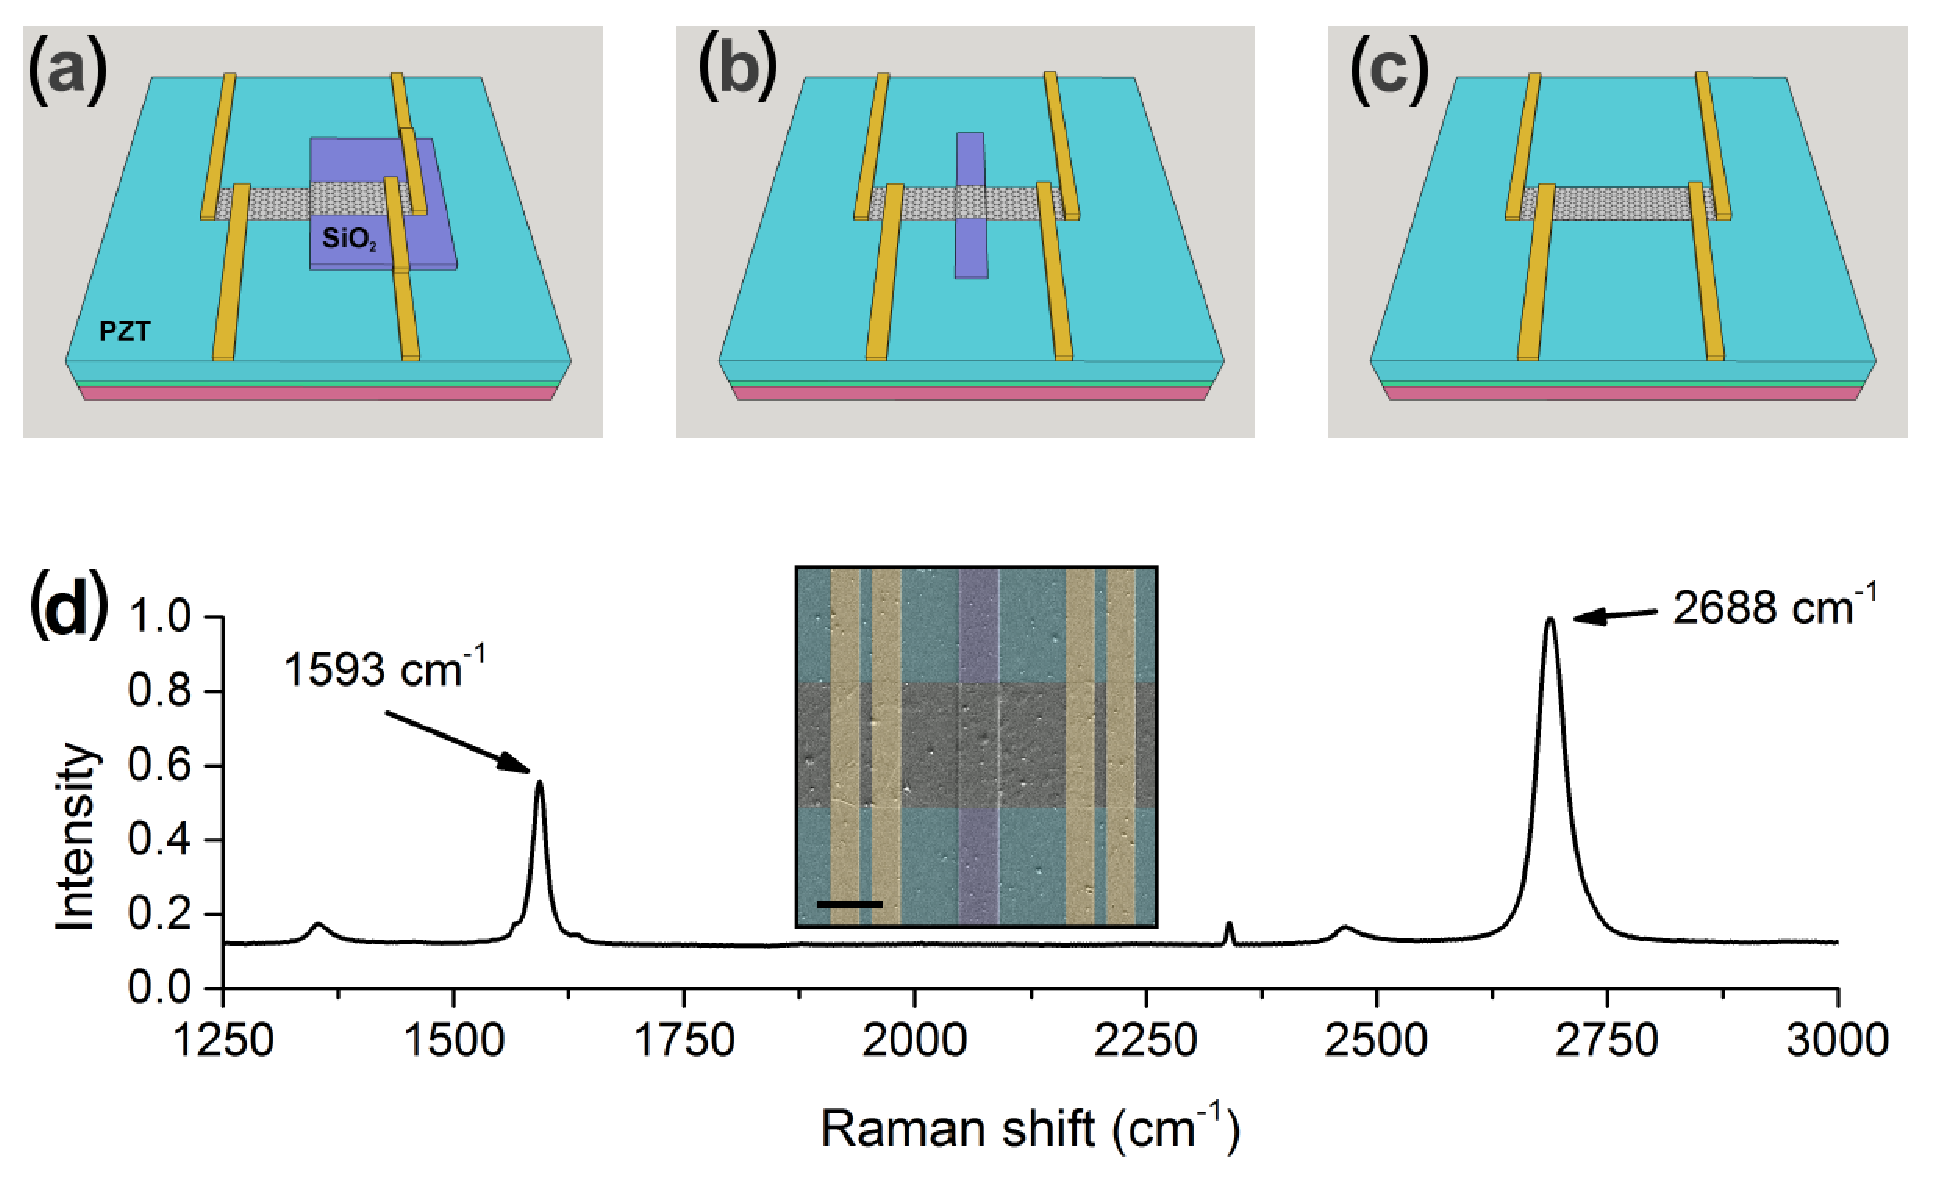
\includegraphics[width=.8\textwidth]{images/resultsanddiscussion/pztpaper/figure1}
  \caption[Schematic illustration of graphene-ferroelectric pn junction device geometry]{
   (a-c) Schematic illustration of the device geometry. The graphene (grey) spans the regions of evaporated SiO$_2$ (purple) on the bare substrate (teal) and is contacted by Cr/Au electrodes (yellow). The universal backgate is shown in red.
   (d) Raman spectra of graphene from a device fabricated on a thermal SiO$_2$ substrate. %The relative intensities of the G and 2D peaks, at 1593 cm$^{-1}$ and 2688 cm$^{-1}$ respectively, and the shape of the G peak confirm the monolayer character and high quality of the graphene.
   Inset: a false-color SEM micrograph of a representative device. The scale bar is 2 $\mu$m.
  }
  \label{fig:devices}
\end{figure}

Transport measurements in air are performed using two Keithley 2400 SourceMeters. Measurements in vacuum are performed using an Agilent 4156C Semiconductor Parameter Analyzer. In both cases source-drain current is measured with a constant source-drain bias of 5 mV while the voltage applied to the backgate is swept. Gate leakage distorts transport results for gate voltages more positive than 1.5 V or more negative than -1 V, so gate voltages are limited to this range. Gate voltage sweep rates range from 10 mV/s to 100 mV/s; the data presented here are from sweeps at 100 mV/s. Slower sweep rates yield qualitatively similar results.

%\section*{Results and Discussion}

    \subsection{Variable local doping via substrate modifications}
    
        Figure \ref{fig:PZTdata}a shows room temperature $I_{sd}$ vs $V_{gate}$ curves for devices having different widths of evaporated SiO$_2$ on a PbZr$_{0.2}$Ti$_{0.8}$O$_3$ substrate. For the data shown here, the fraction of the graphene channel screened by evaporated SiO$_2$ ranges from 0\% to 50\% (corresponding to SiO$_2$ widths of 0 to 3 microns). Two features of the data are immediately apparent: first, for devices which span an evaporated SiO$_2$ region, the characteristic conductance minimum typically observed in graphene at the Dirac point is split into two distinct minima, one at the original Dirac point location and a second shifted to the right. This is apparent in the top and bottom curves of the Figure: the bottom curve, corresponding to a device with 0\% screening, displays a single minimum, while the top curve, corresponding to a device with 50\% screening, displays two pronounced minima. Second, the width of the evaporated SiO$_2$ region determines which of the two minima has a smaller absolute value. As the screening fraction is increased, `weight' is transferred from the minimum at the original Dirac point location to the secondary minimum, and the depths of the two minima vary accordingly. We attribute both of these effects to the presence of two different doping regions in the graphene, defined by the PbZr$_{0.2}$Ti$_{0.8}$O$_3$ substrate and the evaporated SiO$_2$.

        The data can be understood by considering that as the gate voltage is swept from negative to positive, the Fermi level passes through the charge-neutrality point (CNP) of each graphene region separately. Taking the conductance to be linear with carrier density\cite{Hwang2007} $\sigma \propto k_F \langle\tau\rangle \propto n$ and the carrier density to be linear with the thermally smeared energy difference between the Fermi level and the CNP\cite{CastroNeto2009}, we model the conductance in the vicinity of the CNP as: $\rho^{-1} \propto n \propto 1 - e^{{-(V_{gate}}-\mu-\delta)^2/2c^2} + \epsilon$ where the constant $\mu$ accounts for the extrinsic doping introduced by the fabrication process, $\delta \in \{0,1\}$ describes the substrate-dependent doping, and $\epsilon$ accounts for the non-vanishing carrier density at the CNP. Assuming diffusive transport in the graphene, the relative weight of each separately doped region, and therefore the relative magnitude of the measured conductance minima, is determined by the fraction of the graphene channel which is screened:
        \begin{equation}
            I_{sd} \propto \left[ \rho_\text{scr.} \times (\text{pct.}_\text{scr.}) + \rho_\text{non-scr.} \times (\text{pct.}_\text{non-scr.}) \right]^{-1}
        \end{equation}
        This is simulated in Figure \ref{fig:PZTdata}b which shows $I_{sd}$ vs $V_{gate}$ curves for screening fractions ranging from 0\% to 75\% and is in excellent agreement with our experimental data. We note that the simulations agree with our data for $\mu > 0$ and $\delta \geq 0$, which is consistent with the extrinsic p-doping typically observed in graphene devices fabricated on PbZr$_{0.2}$Ti$_{0.8}$O$_3$\cite{Baeumer2013}.

\begin{figure}[!b]
  \centering
  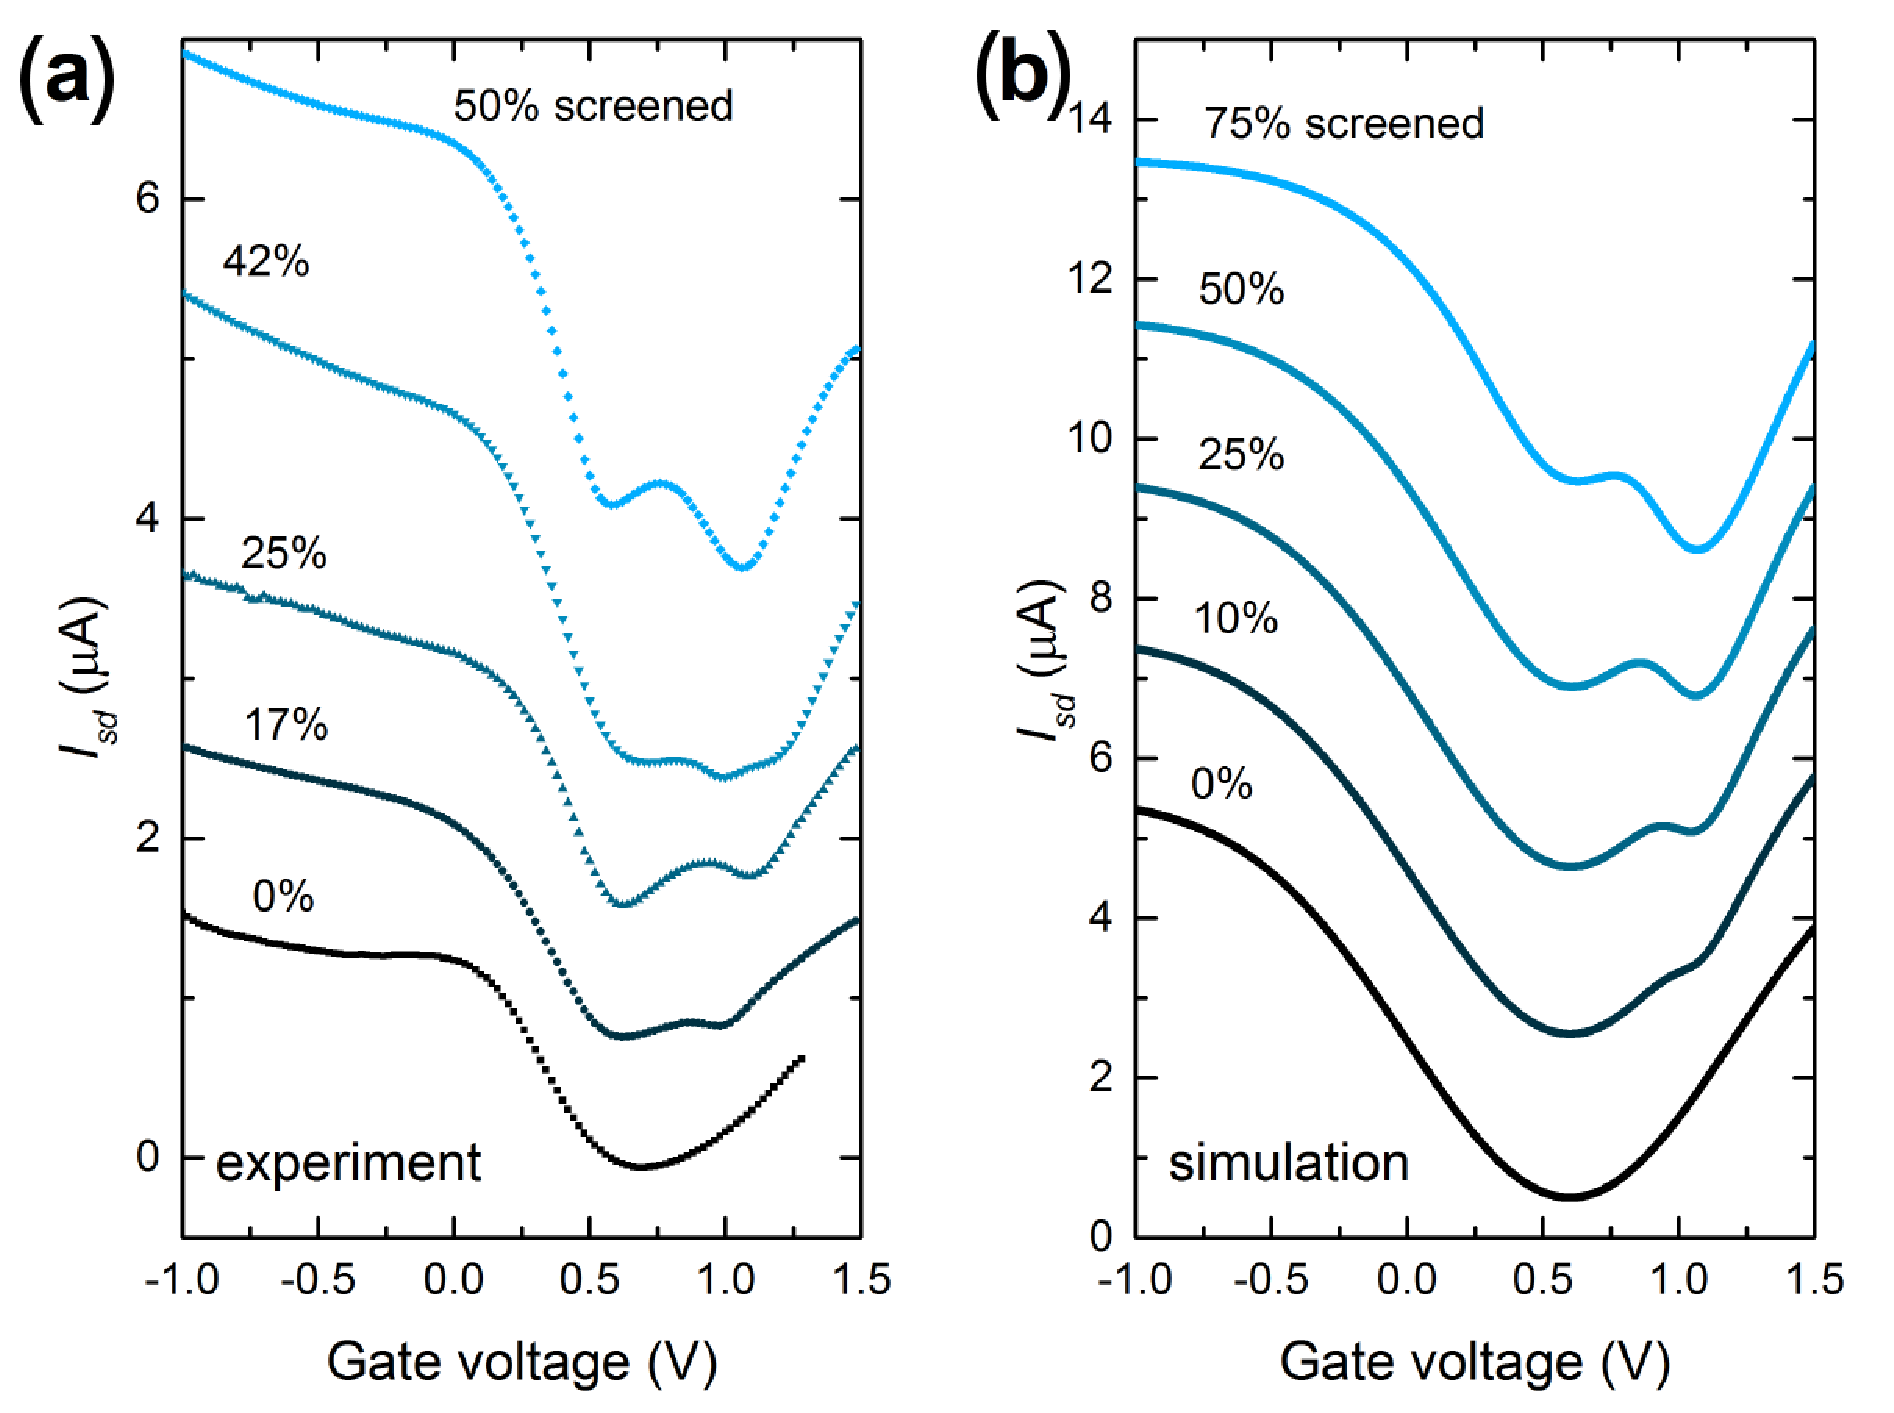
\includegraphics[width=.8\textwidth]{images/resultsanddiscussion/pztpaper/figure2}

  \caption[I-V curves for graphene-ferroelectric pn junction devices]{
   (a) $I_{sd}$ vs $V_{gate}$ curves (manually offset for clarity) for devices having different widths of evaporated SiO$_2$ on a PbZr$_{0.2}$Ti$_{0.8}$O$_3$ substrate. The devices having evaporated SiO$_2$ show split Dirac points, and the relative dominance of the left and right Dirac points can be tuned by varying the evaporated SiO$_2$ width.
   (b) Simulations of transport across a graphene device having two different locally doped regions, as a function of applied gate voltage. The simulations show both Dirac point splitting and variations in left vs. right Dirac point dominance as a function of screening region width, consistent with the experimental data.
}
\label{fig:PZTdata}
\end{figure}

        The substrate-selectivity of the doping in our devices suggests that the ambient dopants are polar H$_2$O molecules. Polar surface adsorbates have been shown to dramatically affect the electronic properties of complex oxide systems\cite{Xie2011} as well as graphene\cite{Schedin2007, Lohmann2009,Lu2014}. The H$_2$O doping is substrate-selective because of the unique ferroelectric nature of the PbZr$_{0.2}$Ti$_{0.8}$O$_3$ substrate. Previous work\cite{Leenaerts2007,Leenaerts2009} has established the importance of the orbital structure of the adsorbate in determining the most energetically favorable orientation. For standard graphene devices on SiO$_2$ substrates, the structure of H$_2$O favors a uniform polarization throughout the range of applicable gate voltages. For graphene on ferroelectric substrates however, previous work\cite{Lu2014} indicates that electrostatic effects of the remnant polarization and substrate lattice geometry can modulate the stability of the H$_2$O polarization. In the devices described here, it is likely that the interaction between the remnant polarization of the PbZr$_{0.2}$Ti$_{0.8}$O$_3$ substrate and the H$_2$O molecules sufficiently alters the energetics of different H$_2$O orientations as to destroy the stability of the H$_2$O polarization, and thus create less-polarized regions. This hypothesis is in agreement with data collected from similar devices fabricated on non-ferroelectric substrates; such devices show none of the characteristic Dirac point splitting associated with p-n junctions.

    \subsection{Hysteresis in local doping}
    
        The gate-voltage dependence of the H$_2$O polarization configurations on PbZr$_{0.2}$Ti$_{0.8}$O$_3$ vs SiO$_2$ leads to hysteresis in the devices. This can be seen in figure \ref{fig:doping_dynamics}a, which shows $I_{sd}$ vs $V_{gate}$ curves for forward and reverse gate sweeps performed on the same devices as measured in Fig. \ref{fig:PZTdata}a. A pronounced hysteresis between forward and reverse gate sweeps is apparent. As in Fig. \ref{fig:PZTdata}a, devices spanning a region of evaporated SiO$_2$ display two distinct minima during forward sweeps, while a control device having no SiO$_2$ displays a single minimum. However, all devices display a single minimum during reverse gate sweeps. We note that the gate voltages applied here remain below the coercive voltage of the PbZr$_{0.2}$Ti$_{0.8}$O$_3$ film, therefore ferroelectric switching is not a possible cause of the observed hysteresis. Ferroelectric switching has been shown to produce similar behavior\cite{Park2015b}, however in this work gate voltages above the coercive voltage of the film are experimentally inaccessible due to large gate leakage in our devices.

        In order to understand how the hysteresis is related to the different H$_2$O polarization configurations on the PbZr$_{0.2}$Ti$_{0.8}$O$_3$ as compared to the evaporated SiO$_2$, it is instructive to consider the gate voltages at which the various minima appear. For example, for the 17\% screened curve in Fig. \ref{fig:doping_dynamics}a the red arrows point out two minima on the forward sweep (at 0.6 V and 1.1V) and one minimum on the reverse sweep (at 0.9 V). These can be compared to the position of the Dirac point in vacuum at 0.6 V (see Fig. \ref{fig:PZTvacuum}). The minimum on the forward sweep at 0.6 V occurs at the same gate voltage as the vacuum Dirac point, implying that it corresponds to a region of the graphene without a net polarization in the adsorbed H$_2$O. The remaining minima occur at voltages larger than the Dirac point (0.9 V and 1.1 V) and thus correspond to regions of the graphene on which the adsorbed H$_2$O is polarized and produces p-doping. Polarized H$_2$O typically produces p-doping in graphene, though the precise mechanism is the subject of continuing research\cite{Leenaerts2007,Moser2008,Wang2010,Wehling2008,Sabio2008}. We identify the forward-sweep minimum at 0.6 V as corresponding to graphene on the non-screened PbZr$_{0.2}$Ti$_{0.8}$O$_3$ region. This is supported by the fact that all devices demonstrate a minimum at 0.6 V, independent of different SiO$_2$ screening fractions. In contrast, the minimum indicated by the rightmost arrow (e.g. at 1.1 V for the 17\% screened device) corresponds to graphene on the evaporated SiO$_2$ region, as evidenced by its evolution with increasing SiO$_2$ screening fraction.

\begin{figure}
  \centering
  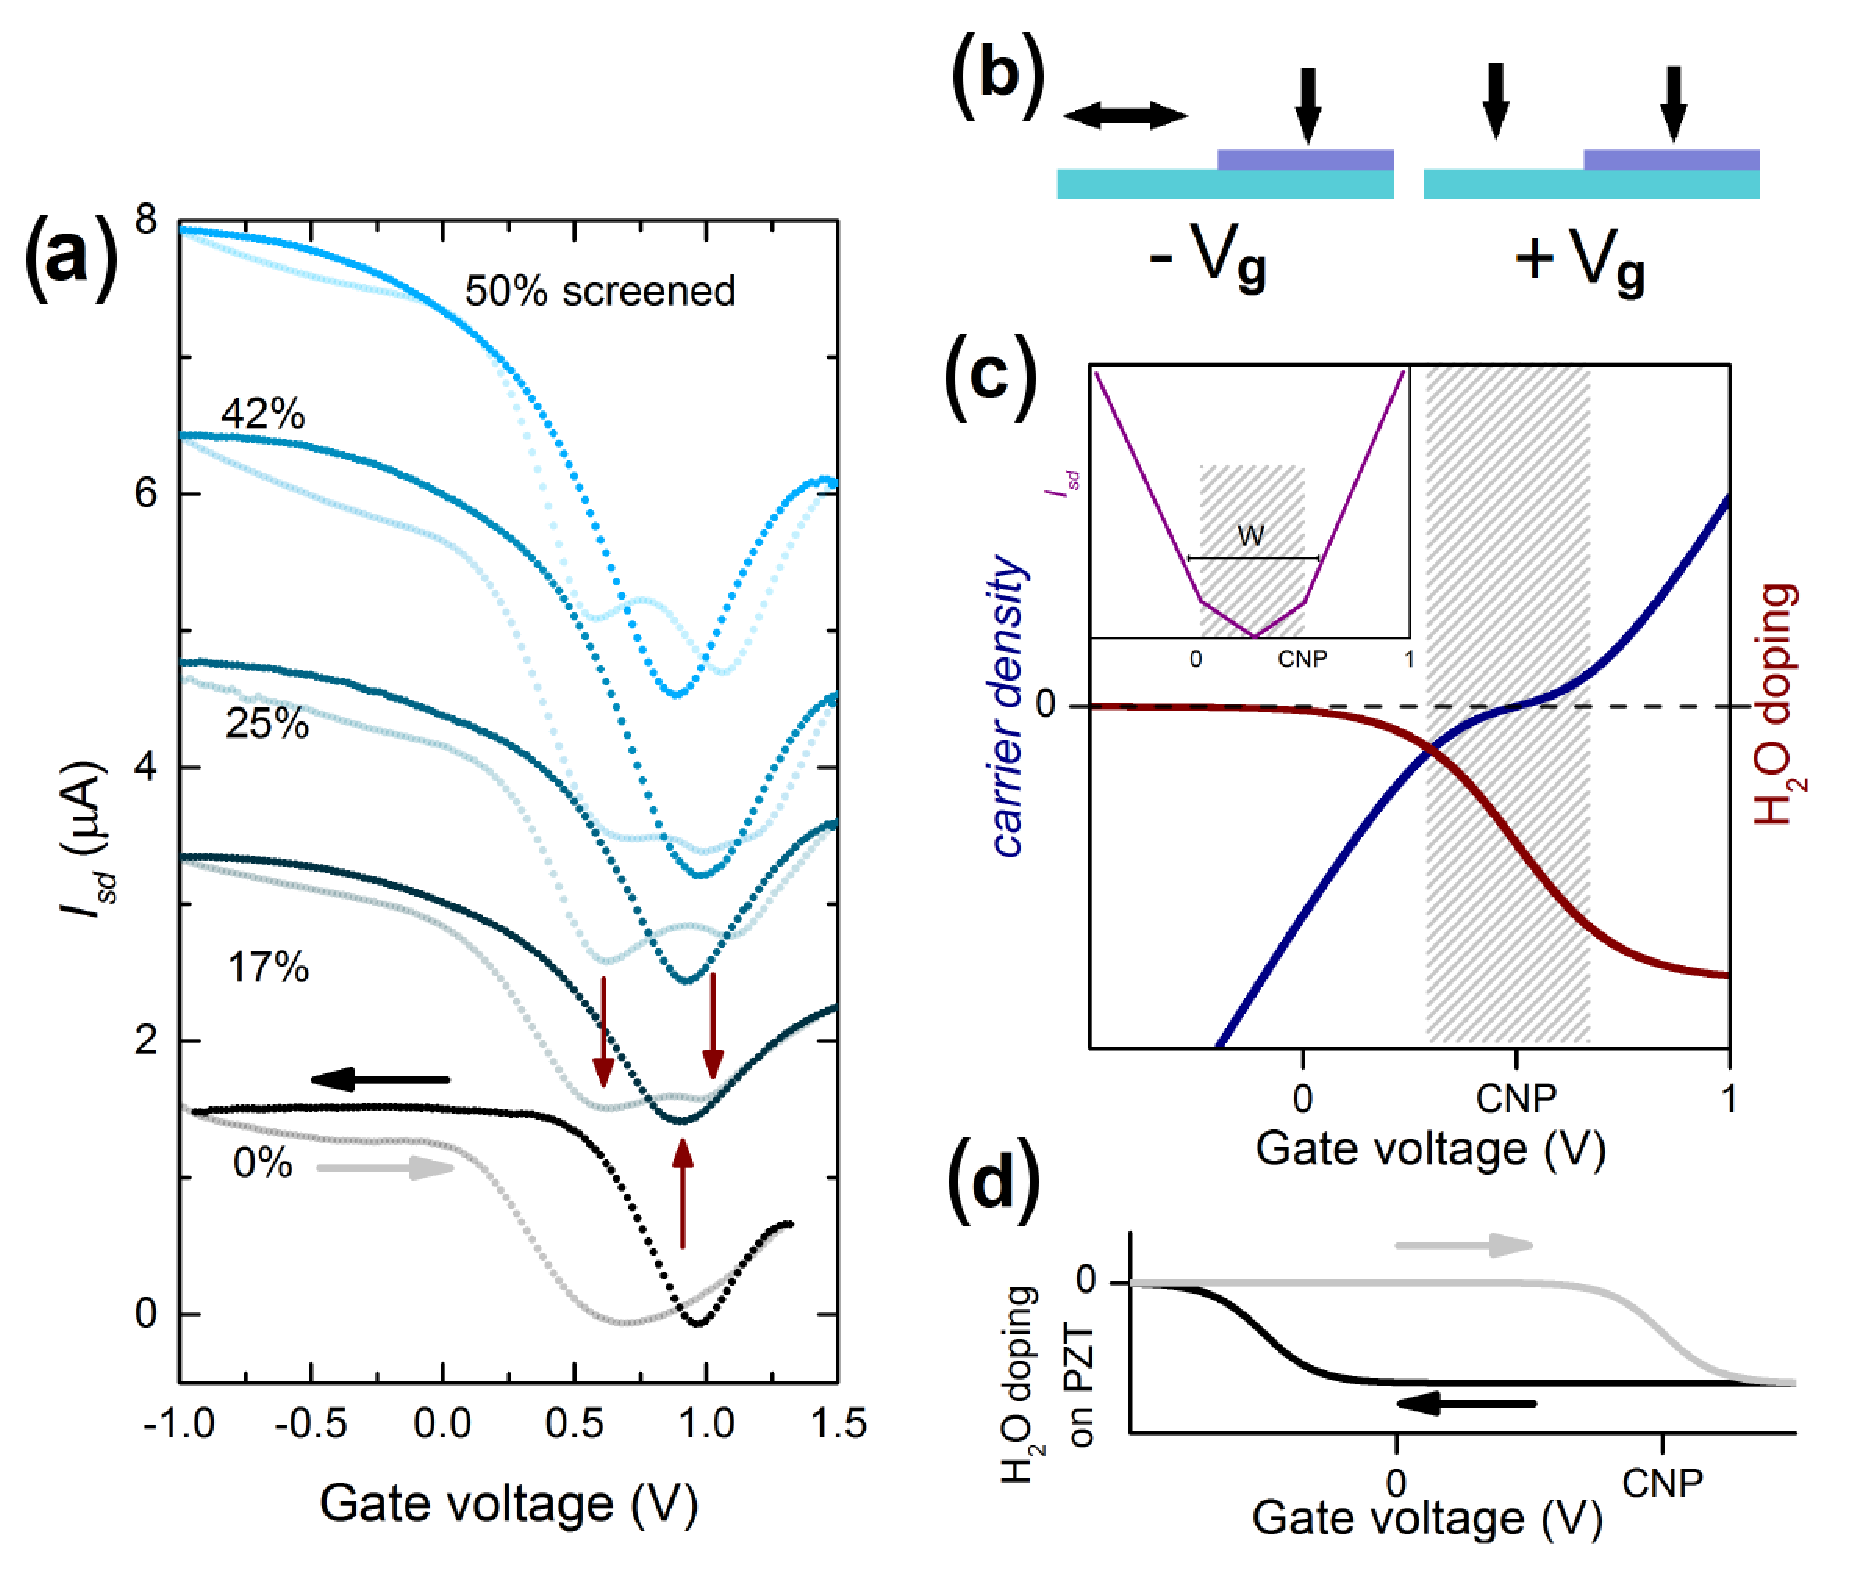
\includegraphics[width=.8\textwidth]{images/resultsanddiscussion/pztpaper/figure3}

  \caption[Polariztion induced hysteresis in I-V curves on graphene-ferroelectric pn junctions]{
   (a) $I_{sd}$ vs $V_{gate}$ curves (manually offset for clarity) for forward (light) and reverse (dark) gate voltage sweeps. Representative minima locations are indicated by the vertical arrows.
   (b) H$_2$O polarization by device region, as prepared by positive and negative gate voltages. For negative gate voltages, H$_2$O on the PbZr$_{0.2}$Ti$_{0.8}$O$_3$ region is unpolarized, and H$_2$O on the SiO$_2$ region is polarized. For positive gate voltages both regions have a net polarization.
   (c) Simulated carrier density vs. applied gate voltage. The onset of H$_2$O polarization is indicated by grey shading. Inset: simulated conductance vs. applied gate voltage.
   (d) A schematic illustration of the H$_2$O doping hysteresis with applied gate voltage; arrows indicate the direction of the gate voltage sweep.
  }
  \label{fig:doping_dynamics}
\end{figure}

    \subsection{Polar adsorbates as local dopants}
    
        We conclude that the application of a negative gate voltage destroys the net polarization of adsorbed H$_2$O on PbZr$_{0.2}$Ti$_{0.8}$O$_3$, but preserves a net polarization on the SiO$_2$-screened regions. This creates different local doping levels and thus a p-n junction. A positive gate voltage establishes a net polarization in both regions, and thus a uniform channel with no p-n junction, as depicted in Figure \ref{fig:doping_dynamics}b. This interpretation is further corroborated by the different widths of the forward and reverse minima for the control (0\% screened) device, as evident in Fig. \ref{fig:doping_dynamics}a. This difference can be explained by considering that conductance is linear with carrier density\cite{Hwang2007}, so the width of the conductance minimum at the Dirac point is determined by the slope of the carrier density vs. gate voltage curve. Typically the slope is constant, determined by the gate capacitance. However, for our devices the onset of H$_2$O dipole doping introduces a nonlinearity in the regime where the adsorbed H$_2$O transitions from unpolarized to polarized; this is shown schematically in Fig. \ref{fig:doping_dynamics}c. The polarized H$_2$O in our devices p-dopes the graphene, so the onset of its doping contribution temporarily reduces the slope of the carrier density vs. gate voltage curve, broadening the conductance minimum. During reverse sweeps, the transition from polarized to unpolarized H$_2$O occurs far from the CNP, so the width of the conductance minimum is unaffected. The hysteresis in H$_2$O polarization is illustrated schematically in Figure \ref{fig:doping_dynamics}d. Experimentally, the polarization hysteresis displays a dependence on both the magnitude of the applied gate voltage and the duration of its application, which prevents an exact determination of the gate voltages required to establish or destroy the H$_2$O polarization.

        The hysteresis of the H$_2$O polarization on PbZr$_{0.2}$Ti$_{0.8}$O$_3$ substrates adds an `on/off' switching element to the p-n behavior. Specifically, we can selectively transition the device into and out of the p-n junction configuration through the application of large positive and negative gate voltages. The initial application of a large positive gate voltages establishes a uniform polarization across the device, yielding a unipolar conducting channel, while a large negative gate voltage destabilizes the polarization on regions supported by PbZr$_{0.2}$Ti$_{0.8}$O$_3$. In the latter case the different H$_2$O polarizations create separate locally doped regions, and thus a p-n junction. This `on/off' switching is different than the standard gate induced switching observed in p-n junctions, for example from p-n to p$^+$-p. By comparison, in our devices the same applied gate voltage can generate either a p-n junction or a uniformly doped channel, depending on the H$_2$O polarization condition.

        The ferroelectric nature of the PbZr$_{0.2}$Ti$_{0.8}$O$_3$ substrate might suggest that the residual electric field from the substrate polarization dopes the regions of graphene in direct contact with the substrate\cite{Baeumer2013,Zheng2010}, but has less effect in the graphene regions screened by evaporated SiO$_2$. Similarly, graphene-ferroelectric interfaces are known to have complex interfacial charge trap dynamics which can generate similar transport signatures\cite{Park2015b}. However, both explanations are precluded by several further experimental observations. First, the Dirac point splitting effect disappears when the devices are measured in vacuum. Figure \ref{fig:PZTvacuum} shows $I_{sd}$ vs $V_{gate}$ curves for the same devices measured at $5\times10^{-6}$ Torr but otherwise under conditions identical to those of Figure \ref{fig:PZTdata}a. All devices show a single minimum, independent of evaporated SiO$_2$ width or gate sweep rate. Second, leaving the devices in ambient conditions overnight recovers the splitting effect. The observed behavior is consistent with an ambient dopant mechanism, i.e., the substrate-selective formation of a self-assembled layer of dopant molecules. In vacuum, dopant molecules desorb from the surface leaving all regions of the graphene identically doped. Leaving the device in ambient conditions allows the dopant layer to reassemble, thereby re-establishing the separately doped regions.

        The absence of Dirac point splitting in vacuum measurements also eliminates differences in gate capacitance as a dominant source of the splitting effect. The screened and non-screened regions of the device have different gate thicknesses and dielectric constants, which might suggest that the application of the same gate voltage would generate different doping levels in each region, and hence the transport behavior we observe. However, any capacitative differences between the regions are static, depending only on the geometry of the device, while the Dirac point splitting effect is dynamic, disappearing in vacuum. Capacitance-based explanations are further ruled out by the nearly identical Dirac point locations observed in all devices under vacuum. In particular, the similarity of data under vacuum from the control device (having no evaporated SiO$_2$), and from the devices which do span an evaporated SiO$_2$ region confirms that gate capacitance differences between the two regions are not the primary cause of the Dirac point splitting effect.


\begin{figure}
  \centering
  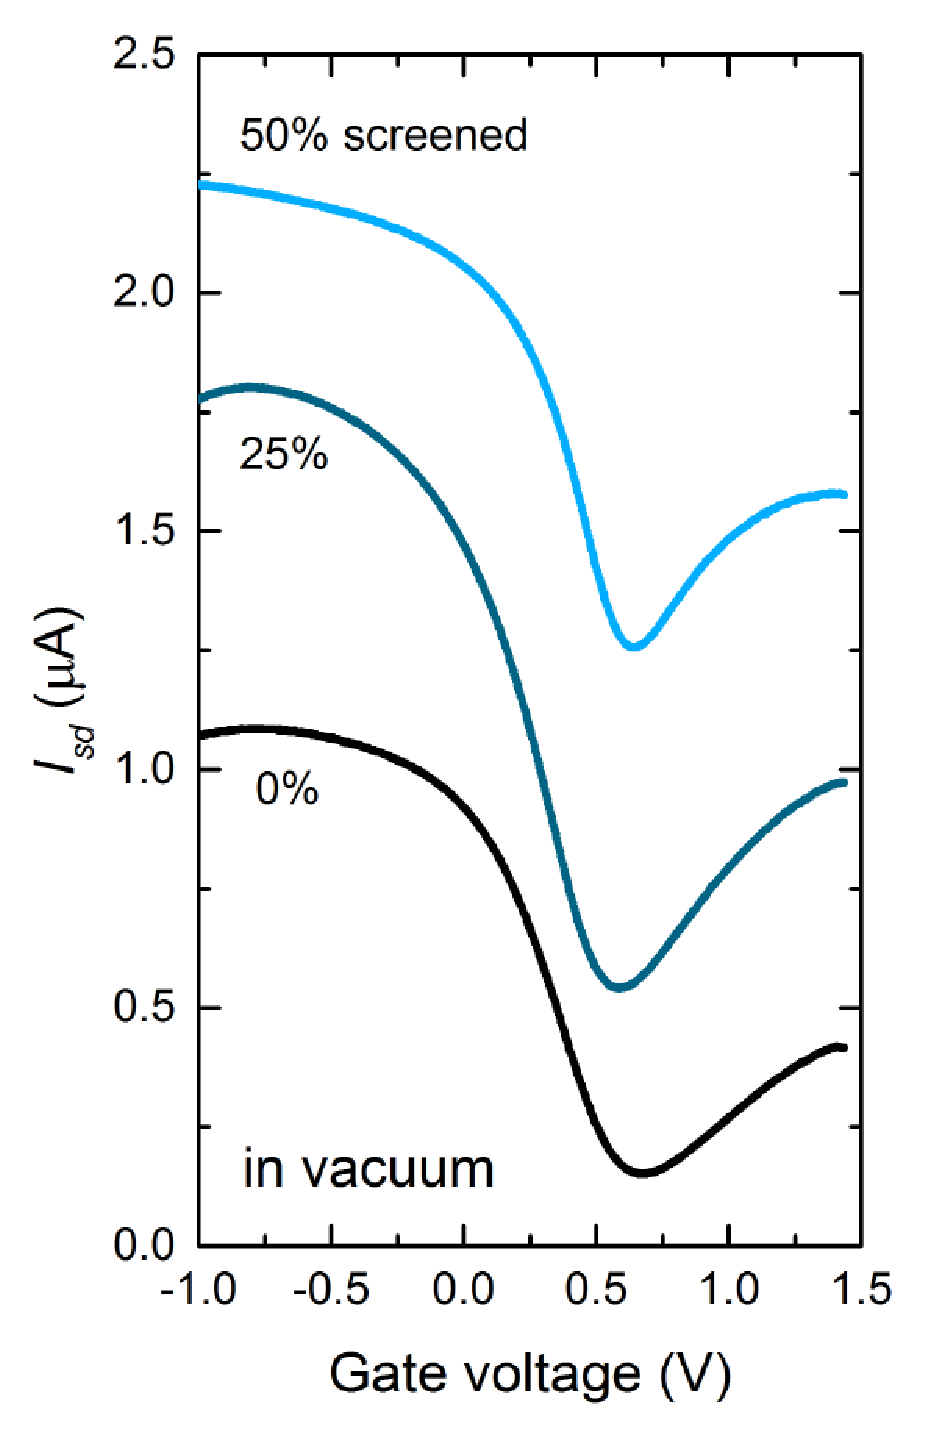
\includegraphics[width=.5\textwidth]{images/resultsanddiscussion/pztpaper/figure4}
  \caption[I-V curves for graphene-ferroelectric pn junction devices measured in vacuum]{
   Offset $I_{sd}$ vs $V_{gate}$ curves for devices measured in vacuum. The Dirac point splitting effect disappears in vacuum, but can be recovered by leaving the device in ambient conditions overnight.
  }
  \label{fig:PZTvacuum}
\end{figure}

        We note that the vacuum-dependence of our results requires that the ambient dopant molecules be present on top of the graphene rather than trapped between the graphene and the substrate. Pristine monolayer graphene is impermeable to atomic and molecular species\cite{Bunch2008}, therefore the brief application of a moderate vacuum would be insufficient to remove any molecules trapped underneath the graphene. This in turn requires that the substrate-dependent localization of the ambient dopants occurs through the graphene; similar behavior has been previously reported elsewhere\cite{Moser2007, Moser2008, Lohmann2009, Lafkioti2010}.

%\section*{Conclusions}

    \subsection{Summary}

        In summary, we have fabricated a controllable p-n junction in graphene on a ferroelectric substrate. We employ simple substrate modifications to define local doping regions, where the doping is accomplished through the substrate-selective formation of a self-assembled layer of ambient doping molecules. Alternative explanations for the local doping effect are ruled out, and the dynamics of the ambient doping suggest that it is due to polar H$_2$O molecules. Finally, the PbZr$_{0.2}$Ti$_{0.8}$O$_3$ substrate creates a hysteresis in the ambient doping effect which can be used to controllably bias the device into and out of a p-n junction configuration, using a single, universal backgate.

%\section*{Methods}

%\textbf{Transport Measurements.} Transport measurements in air were performed using two Keithley 2400 SourceMeters. Current through the graphene channel was measured under a constant bias of 5 mV, while the gate voltage was swept between -1.0 and +1.5 V. Measurements in vacuum were performed using an Agilent 4156C Semiconductor Parameter Analyzer under identical electrical parameters. In both cases gate voltage sweep rates ranged from 10 mV/s to 100 mV/s; data from different sweep rates yielded qualitatively similar results.

\textit{Acknowledgement.} J.H.H., R.X., S.R., and M.S. acknowledge support from the National Science Foundation and the Nanoelectronics Research Initiative under NSF-NEB grant DMR-1124696.
S.P. acknowledges support from the Army Research Office under grant W911NF-14-1-0104. N.M. and L.W.M. acknowledge support from the National Science Foundation under grant ENG-1434147. This work was carried out in part in the Frederick Seitz Materials Research Laboratory Central Facilities at the University of Illinois.



\section{Graphene on strain array substrates}
    \subsection{Device configuration}


\chapter{Summary and conclusions}
\section{Summary of results}
\section{Future work}

\begin{appendices}

\chapter{Device Fabrication Procedures}
\label{appendix:fab}
\section{Growing CVD graphene}
\section{Graphene on flexible substrates}
\section{Graphene on ferroelectric substrates}

Substrates were prepared by pulsed-laser deposition: strontium titanate (SrTiO$_3$) substrates were first coated with 20 nm of strontium ruthenate (SrRuO$_3$) followed by 120 nm of (001)-oriented lead zirconium titanate (PbZr$_{0.2}$Ti$_{0.8}$O$_3$). The details of the substrate fabrication are discussed in Refs. 
\cite{Xu2014,Karthik2012}.
For each substrate, 80 nm of SiO$_2$ was evaporated in small rectangular regions defined by conventional photolithography. CVD graphene was then transferred onto the substrate using standard wet-transfer techniques as discussed in \cite{Li2009}.
Photolithography was used to define graphene channels which spanned the evaporated SiO$_2$ regions; 
the remainder of the graphene was removed by oxygen plasma etching (60 seconds, 100 W, 200 mtorr, 20 sccm O$_2$). 
Finally, electrical leads were defined in a four-point measurement configuration using photolithography, and 20 nm of gold was deposited by electron-beam evaporation with a 3 nm sticking layer of titanium.

\section{Graphene on strain array substrates}

\chapter{Python Measurement Code}

During the course of this research I became frustrated with the existing instrument control programs
our lab used to perform measurements.
Most of this frustration stemmed from what I perceived to be shortcomings in LabVIEW, the programming
language in which they were implemented. Briefly, these shortcomings are as follows:

    \begin{enumerate}
        \item \textbf{Code modification and reuse:} LabVIEW is a graphical programming language: 
            programs are `written' by connecting boxes representing functions and variables with `wires` which
            pass input and output values. This paradigm makes it nearly impossible to modify
            an existing program of any complexity. To understand the logical flow of the program
            one must trace the paths and connections of upwards of 100 wires, each with multiple forks
            and branches; see Figure \ref{fig:labview} for an example. 
            The result of this is that any existing code can only be used to
            perform the exact same measurement for which it was created; to perform an only slightly 
            different measurement one must create an entirely new program, or invest an equivalent 
            amount of time in debugging changes to an existing program.
        \item \textbf{Commenting and versioning:} LabVIEW does not have robust options for commenting
            or versioning\footnote{`Versioning' refers to the process of tracking changes
            between sequential versions of some code. For example, the Track Changes functionality in Microsoft
            Office is used to version text docuemnts.} code. The lack of commenting exacerbates the difficulty of understanding
            an existing program, and the lack of version control makes it difficult to incrementally
            develop a program. Taken together these shortcomings also require that all meta-information about the
            program must be stored in the program file name, leading to program names like 
            `gate\_sweep\_keithley\_sr830\_jeffs\_edit\_v3\_new\_B\_usethisone.vi'.
        \item \textbf{Version incompatibility:} New versions of LabVIEW are released 
            yearly, however each new version breaks backwards compatibility.
            This causes many, many headaches when trying to run measurement programs inherited
            from previous students in the lab, or when trying to run a new program on a workstation
            with an earlier version of LabVIEW installed.
    \end{enumerate}
        
\begin{figure}
    \centering
    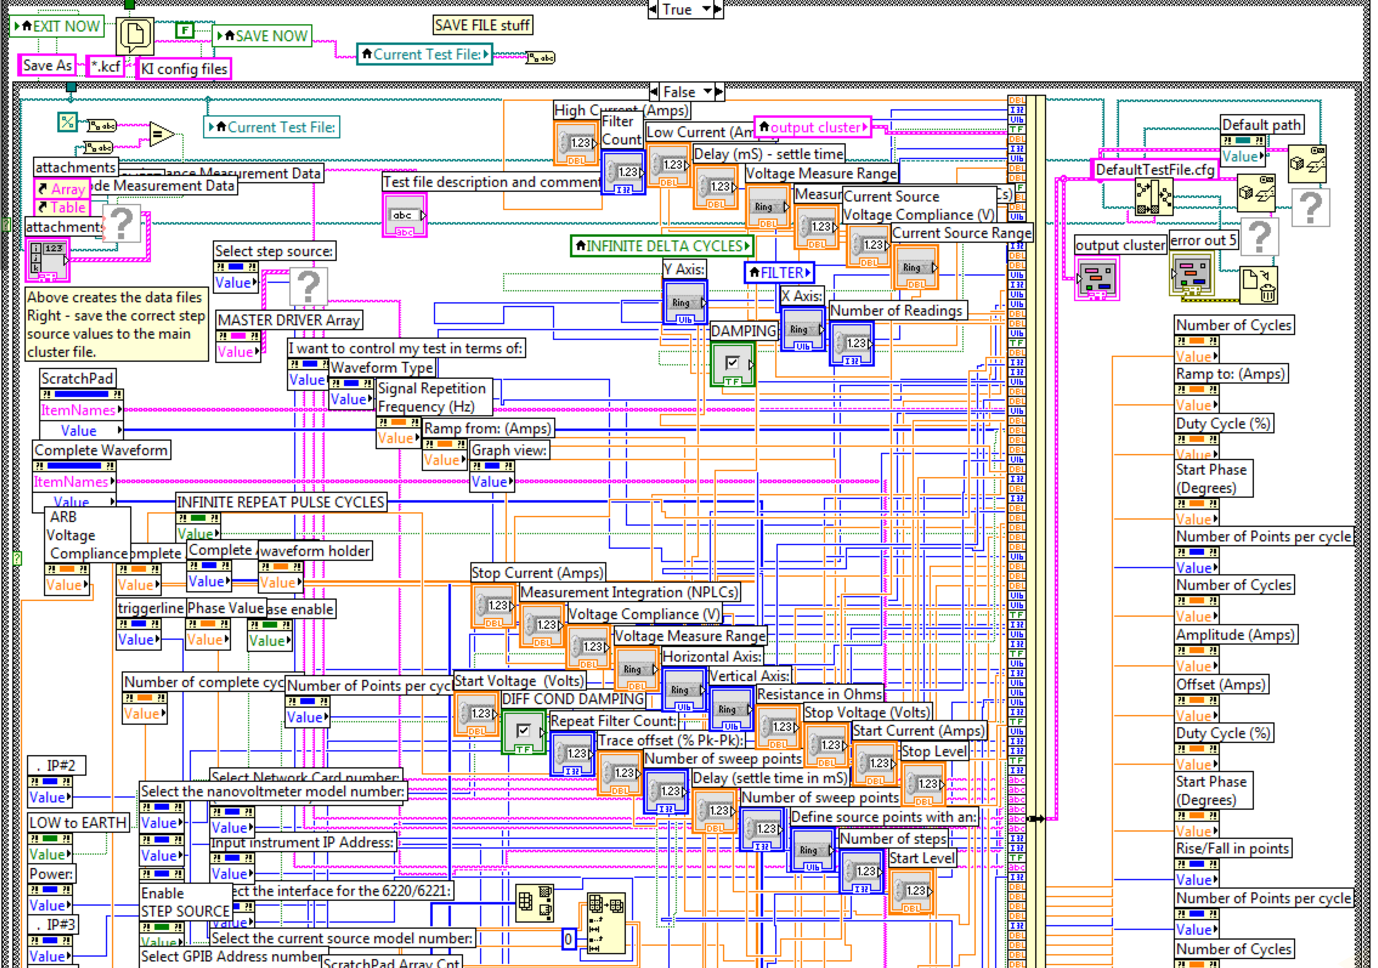
\includegraphics[width=\linewidth]{images/python/labview.png}
    \caption[Example LabVIEW program]{
        A portion of a LabVIEW program. The boxes are functions and variables, 
        and the wires pass input and output values between the functions.
    }
    \label{fig:labview}
\end{figure}
        
Given these frustrations, the obvious question is ``Why use LabVIEW at all?". ``Instrument drivers" is the short answer.
Nearly every conceivable lab instrument provides drivers which allow the instrument to communicate
with LabVIEW. The primary barrier to writing instrument control programs in languages other than
LabVIEW is the absence of instrument drivers in those languages.


\section{Instrument Drivers}

In order to address these issues I wrote drivers in the Python programming language
for most of the instruments in our lab. These drivers can be found at \url{https://github.com/masonlab/labdrivers}
and their usage is documented at \url{http://labdrivers.readthedocs.io/en/latest/}.
In the rest of this section I describe the process used to create these drivers.

    \subsection{Writing new drivers}
    
    The purpose of an instrument driver is to facilitate communication between an instrument and a
    computer. Each instrument has a fixed set of commands it accepts, and a fixed set of outputs it will
    provide upon request. The task when writing a driver is to provide a convenient way to send commands
    and retrieve the relevant data.
    Most instruments provide a complete list of the commands they accept, often at the end of their instruction manual.
    These commands are not convenient for human use however, they are typically short and obscure 
    (``\code{*IDN?}" or ``\code{*RST}" for example).
    The task is to write a set of Python functions with simple, meaningful names which pass the
    appropriate command to the instrument (for example ``\code{get\_instrument\_id}" or ``\code{reset\_instrument}"). 
    For convenience, these functions can then be collected in a
    Python class to group all the functions for a particular instrument.
    
    The majority of the instruments in our lab communicate with a computer using the National Instruments VISA
    standard. This standard describes how commands (like \code{*RST}) get translated into a format interpretable by the instrument.
    Conveniently, there is already a Python library called PyVISA which implements this standard.
    In practice, this means we can pass a command to the PyVISA library, and the library will handle the low-level
    work of passing that command to the instrument in a format it understands.
    Writing a Python instrument driver is thus a three step process:
    \begin{enumerate}
        \item Enumerate the commands which the instrument accepts
        \item Write a python function to pass each instrument command to PyVISA
        \item Collect the python functions into a class
    \end{enumerate}
    Below I demonstrate this process for a single command.
    
    \subsubsection*{Enumerate commands the instrument accepts}
    
        In this example I will write a partial instrument driver for the SR830 lock-in amplifier. The first
        step is to find a listing of the commands which the instrument accepts; for the SR830 such a list
        can be found at the end of the instrument's instruction manual. An excerpt is shown in Figure \ref{fig:sr830manual}.
        \begin{figure}
            \centering
            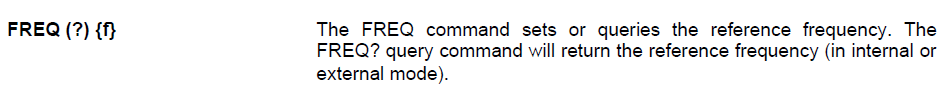
\includegraphics[width=\linewidth]{images/python/sr830.png}
            \caption[Excerpt from the SR830 manual]{
                An excerpt from the manual of the SR830 lock-in amplifier which details one of the 
                commands which the SR830 will accept from a computer.
            }
            \label{fig:sr830manual}
        \end{figure}
        This portion of the manual describes two commands: passing \texttt{FREQ?} to the instrument queries 
        the current frequency, and passing \texttt{FREQ X} where \texttt{X} is some number sets the instrument
        frequency to that number.
    
    \subsubsection*{Write a python function for each command}
    
    The next step is to write a python function which passes this command to the instrument.
    To do this we use the existing PyVISA \href{https://pyvisa.readthedocs.io/en/stable/}{(\textbf{link})} library in python.
    This library facilitates communication between computers and instruments which communicate using the VISA
    standard, which in practice is most instruments. Most of this communication is done using a python class
    from the PyVISA library called \texttt{GPIBInstrument}. This class has two relevant methods: \texttt{write()} and
    \texttt{query()}. The first passes a command to the instrument, and the second passes a command and retrieves
    the response. The general approach here is to create an instance of the \texttt{GPIBInstrument} class 
    and then call \texttt{write()} and \texttt{query()} with appropriate arguments.
    
    Below I demonstrate how to create an instance of the \texttt{GPIBInstrument} class for 
    an instrument having a GPIB address of 14. Note that this tutorial closely follows the 
    PyVISA documentation, available at the link given above.
    \begin{verbatim}
    import visa
    
    GPIB_addr = 14
    
    rm = visa.ResourceManager()
    my_instrument = rm.open_resource('GPIB0::{}::INSTR'.format(GPIB_addr))
    \end{verbatim}
    We can now use this instance of the \texttt{GPIBInstrument} class to communicate with our SR830.
    In this case we will write two functions, one for each of the commands we enumerated above.
    Note that both commands require the existence of the \texttt{my\_instrument} variable which
    we created in the previous code block.
    \begin{verbatim}
        def set_frequency(my_instrument, freq):
            my_instrument.write('FREQ {}'.format(freq))
            
        def get_frequency(my_instrument):
            return my_instrument.query('FREQ?')
    \end{verbatim}
    Now we can call either the functions defined above to get or set the frequency of the SR830.
    
    \subsubsection*{Collect the functions into a class}
    
    The final step is to collect the functions for a given instrument into a python class for that instrument.
    The rationale here is that collecting functions into a class allows us to more logically track multiple
    instruments. This grouping can be accomplished as follows:
    \begin{verbatim}
        class SR830():
        
            def __init__(self, GPIB_addr):
                self.instrument = rm.open_resource('GPIB0::{}::INSTR'.format(GPIB_addr))
                
            def set_frequency(self, freq):
                self.instrument.write('FREQ {}'.format(freq))
                
            def get_frequency(self):
                return self.instrument.query('FREQ?')
    \end{verbatim}
    The code above uses the standard python class definition syntax; for an explanation of that syntax see
    the python documentation.
    
    
    \subsection{Wrapping existing drivers}
    
    The process described above requires that the instrument can be controlled using the VISA standard.
    For instruments where this is not the case, another option is to `wrap' existing drivers which are
    written in other languages. The practical implementation is more complex, but this wrapping process is logically
    similar to the VISA-based process: 
    \begin{enumerate}
        \item Enumerate the commands which the other driver accepts
        \item Write a python function to invoke each command in the existing driver
        \item Collect the python functions into a class
    \end{enumerate}
    Instead of passing commands to the PyVISA library we invoke commands in the existing driver, but otherwise
    the process of creating a Python driver is the same.
    
    The difficulty of wrapping other drivers mostly lies in figuring out how to run commands from another
    programming language (the language that the original driver was written for) from within Python.
    The method required to do this depends on the language of the original driver, however there are often
    existing Python libraries to facilitate this task. A complete accounting of these existing libraries
    is beyond the scope of this thesis, and in fact would likely be immediately out of date;
    the motivated reader is encouraged to Google around. For examples
    of drivers created by this process see the drivers for the National Instruments BNC-2100 DAC
    (\href{https://github.com/masonlab/labdrivers/blob/master/labdrivers/ni/bnc2110.py}{\textbf{link}})
    and the Quantum Design PPMS DynaCool 
    (\href{https://github.com/masonlab/labdrivers/blob/master/labdrivers/quantumdesign/dynacool.py}{\textbf{link}}).
    
    
\section{Example measurement programs}
\subsection{Gate-sweep Example}
\subsection{Field-sweep Example}
\subsection{Sheet Resistance Example}

\end{appendices}

\backmatter

\bibliographystyle{catunsrt}
%\addbibresource{rippingpaper.bib}
%\addbibresource{pztpaper.bib}
%\addbibresource{PrelimPaper.bib}
%\addbibresource{thesis.bib}
\bibliography{rippingpaper,pztpaper,PrelimPaper,thesis}


\end{document}
\endinput
